\documentclass[11pt, spanish]{article}
\usepackage[spanish]{babel}
\selectlanguage{spanish}
\usepackage[utf8]{inputenc}
\usepackage{graphicx}
\usepackage{mathtools}
\usepackage{tabularx}
\usepackage[font=small,labelfont=bf]{caption}
\usepackage{subcaption}
\usepackage{authblk}
\usepackage{natbib}
\usepackage{multirow}


\captionsetup[table]{name=Tabla}
\renewcommand{\thetable}{\Roman{table}}
\newcommand{\mean}[1]{\left\langle#1\right\rangle}
%\newcommand{\eqref}[1]{Ec.~\ref{#1}}

\begin{document}
\begin{titlepage}
    \centering
    {\scshape\LARGE Universidad de Buenos Aires \par}
    \vspace{1cm}
    {\scshape\Large Informe 2:\par}

    \vspace{1.5cm}
    {\scshape\Large\par}
    {\huge\bfseries  Lethalily-Centrality Rule\par}
    \vspace{2cm}
    {\Large\itshape Ra\'ul Barriga\par}
    {\Large\itshape Mariela Celis\par}
    {\Large\itshape Jimmy Mas\'ias\par}
    {\Large\itshape Sebast\'ian Pinto\par}

    \vfill

    \vfill

                                                    % Bottom of the page
    {\large \today\par}
\end{titlepage}

    %--- tabla de contenidos
    \tableofcontents

    \newpage
    \section{Introducci\'on}
El modelo cl\'asico de redes aleatorias de Erd\"os-R\`enyi asume que un par de 
nodos est\'an conectados con una probabilidad $p$, generando redes estadisticamente
homog\'eneas y distribuci\'on de grado tipo Poisson~\citep{jeong2000}. Sin embargo, 
muchas redes complejas reales (como internet~\citep{faloutsos1999} o 
redes metab\'olicas~\citep{jeong2000}) muestran comportamientos libre de 
escala, es decir, se caracterizan por tener pocos nodos altamente conectados 
\textit{hubs} con nodos poco conectados.

En el caso de redes biol\'ogicas, a trav\'es de t\'ecnicas gen\'eticas, se ha 
demostrado la existencia de genes indispensables para la sobrevivencia (genes
\textit{esenciales}) \citep{kamath2003,winzeler1999}. Desde entonces se ha 
buscado una forma de caracterizar la esencialidad de un nodo en una red a 
trav\'es de sus caracter\'isticas topol\'ogicas.

En \citet{jeong2000} se trabaja sobre 43 redes metab\'olicas y reporta una 
correlaci\'on entre los hubs de la red y la esencialidad del nodo desde 
el punto de vista biol\'ogico. A esta correlaci\'on la llamaron 
\textit{regla de Centralidad-Letalidad} (Centrality-Lethality rule) y 
posteriormente este trabajo ha sido reportado numerosas veces por otros 
autores. La principal cr\'itica que ha recibido esta correlaci\'on es al ser
considerada muchas veces como raz\'on causal, es por ello que en
\citet{he2006} se plantea una aproximaci\'on distinta al problema, pero 
con consecuencias equivalentes. En \citet{he2006} se establece que la
esencialidad de un nodo (i.e. prote\'ina) se debe a la participaci\'on de 
este en una interacci\'on/proceso (conexiones) esencial, luego debido 
a que los hubs tienen una alta conectividad con otros nodos, es m\'as 
probable que una de sus interacciones sea esencial.


El presente estudio es una revisi\'on del trabajo de \citet{zotenko2008} en que 
se estudia las debilidades de las hip\'otesis de Jeong y He. Para ello utilizamos
cuatro redes proteicas de levadura (\textit{S. cerevisiae}): Obtenida a partir 
de Affinity-Purification/Mass-Spectrometry (AP-MS) \citep{apms_data}, de 
interacciones binarias yeast two-hybrid (Y2H) \citep{y2h_data} y dos curadas 
de literatura \citep{lit_data}. Los datos para 
construir las redes fueron obtenidos de la \textit{Yeast Interactome Database}.


    \newpage
    
\section{Caracterizaci\'on}

Siguiendo el trabajo de \citet{zotenko2008} tomamos cuatro redes de interacci\'on de levadura (\textit{Saccharomyces cerevisiae}) disponibles en el Yeast Interactome Database\footnote{http://interactome.dfci.harvard.edu/S\_cerevisiae/}. Estas redes fueron obtenidas a partir de diferentes t\'ecnicas: a trav\'es de Affinity-Purification/Mass-Spectrometry (AP-MS) \citep{apms_data}; de 
interacciones binarias Yeast Two-Hybrid (Y2H) \citep{y2h_data} y dos curadas de literatura \citep{lit_data} {\bf (FALTA UNA CITA AQUI)}. La figura \ref{grafos} muestra una representaci\'on gr\'afica de las cuatro redes consideradas.


% La idea del ejercicio es realizar un analisis cuantitativo de las tres redes y observar las coherencia entre las interacciones reportadas


\begin{figure}[!ht]
    \centering
    \begin{subfigure}[b]{0.4\columnwidth}
        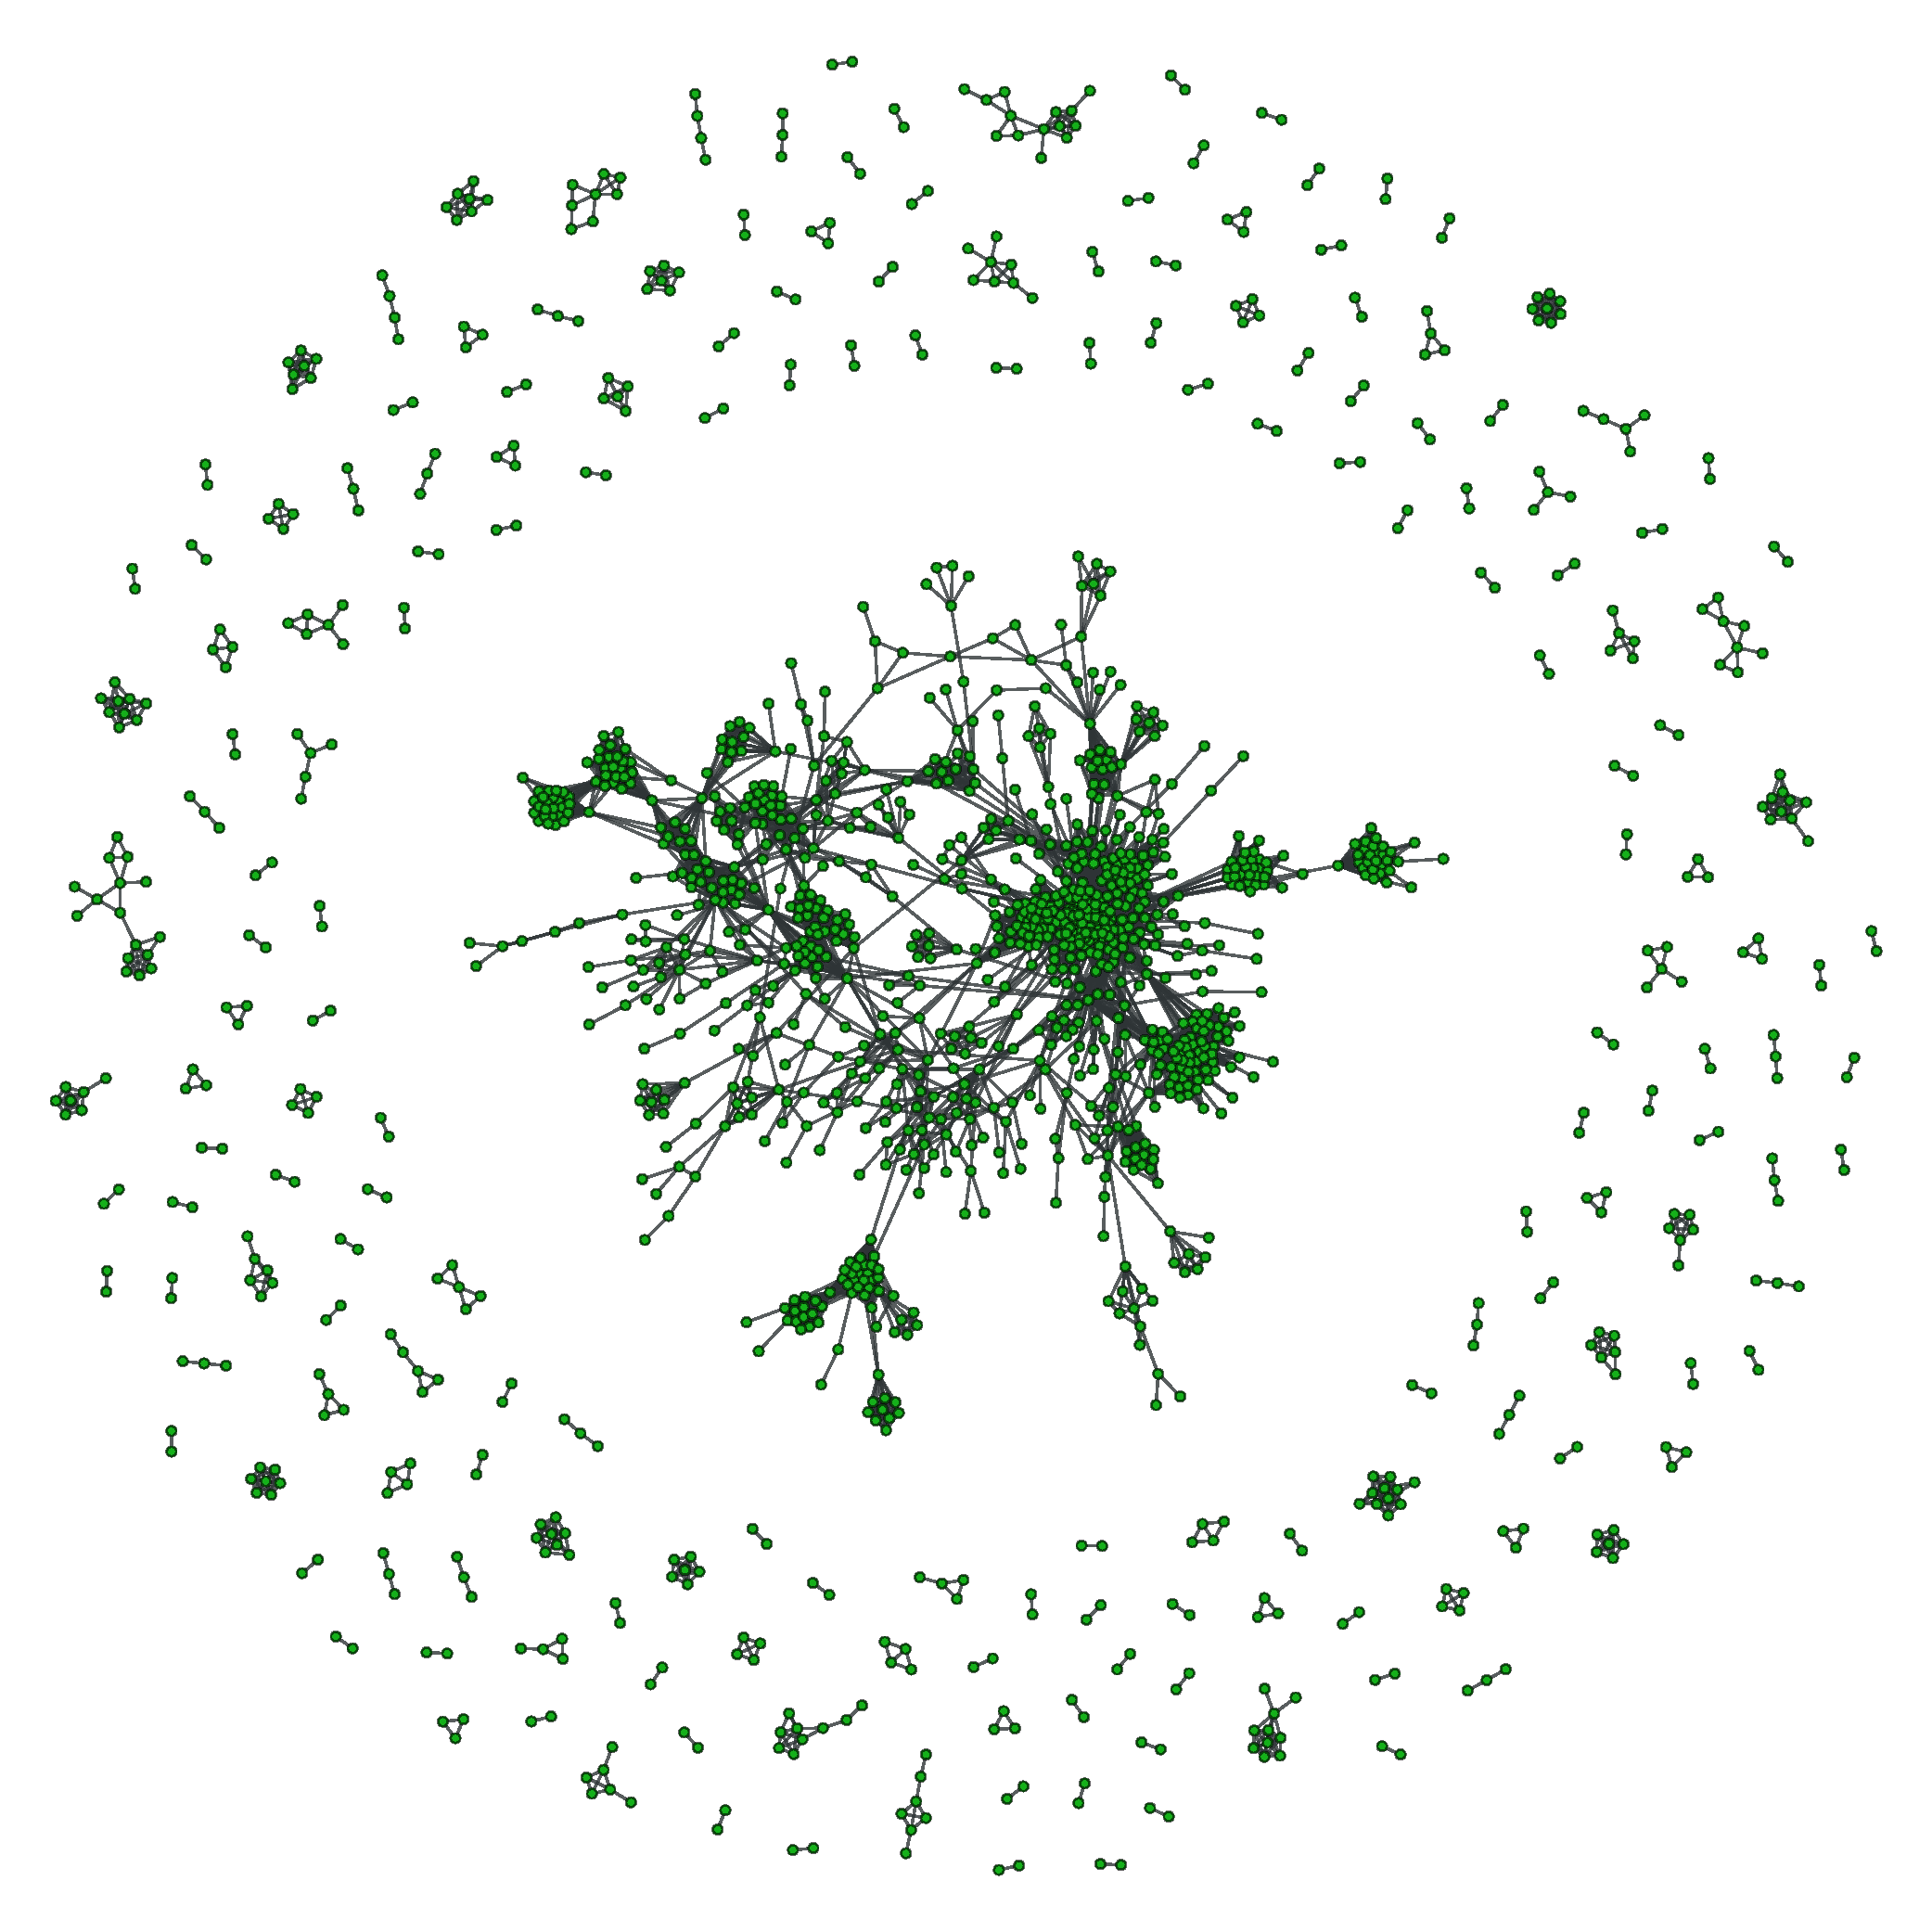
\includegraphics[width=\textwidth]{./schemes/yeast_AP-MS-txt.pdf}
        \caption{\label{fig:ap_ms} AP-MS}
    \end{subfigure}
    \begin{subfigure}[b]{0.4\columnwidth}
        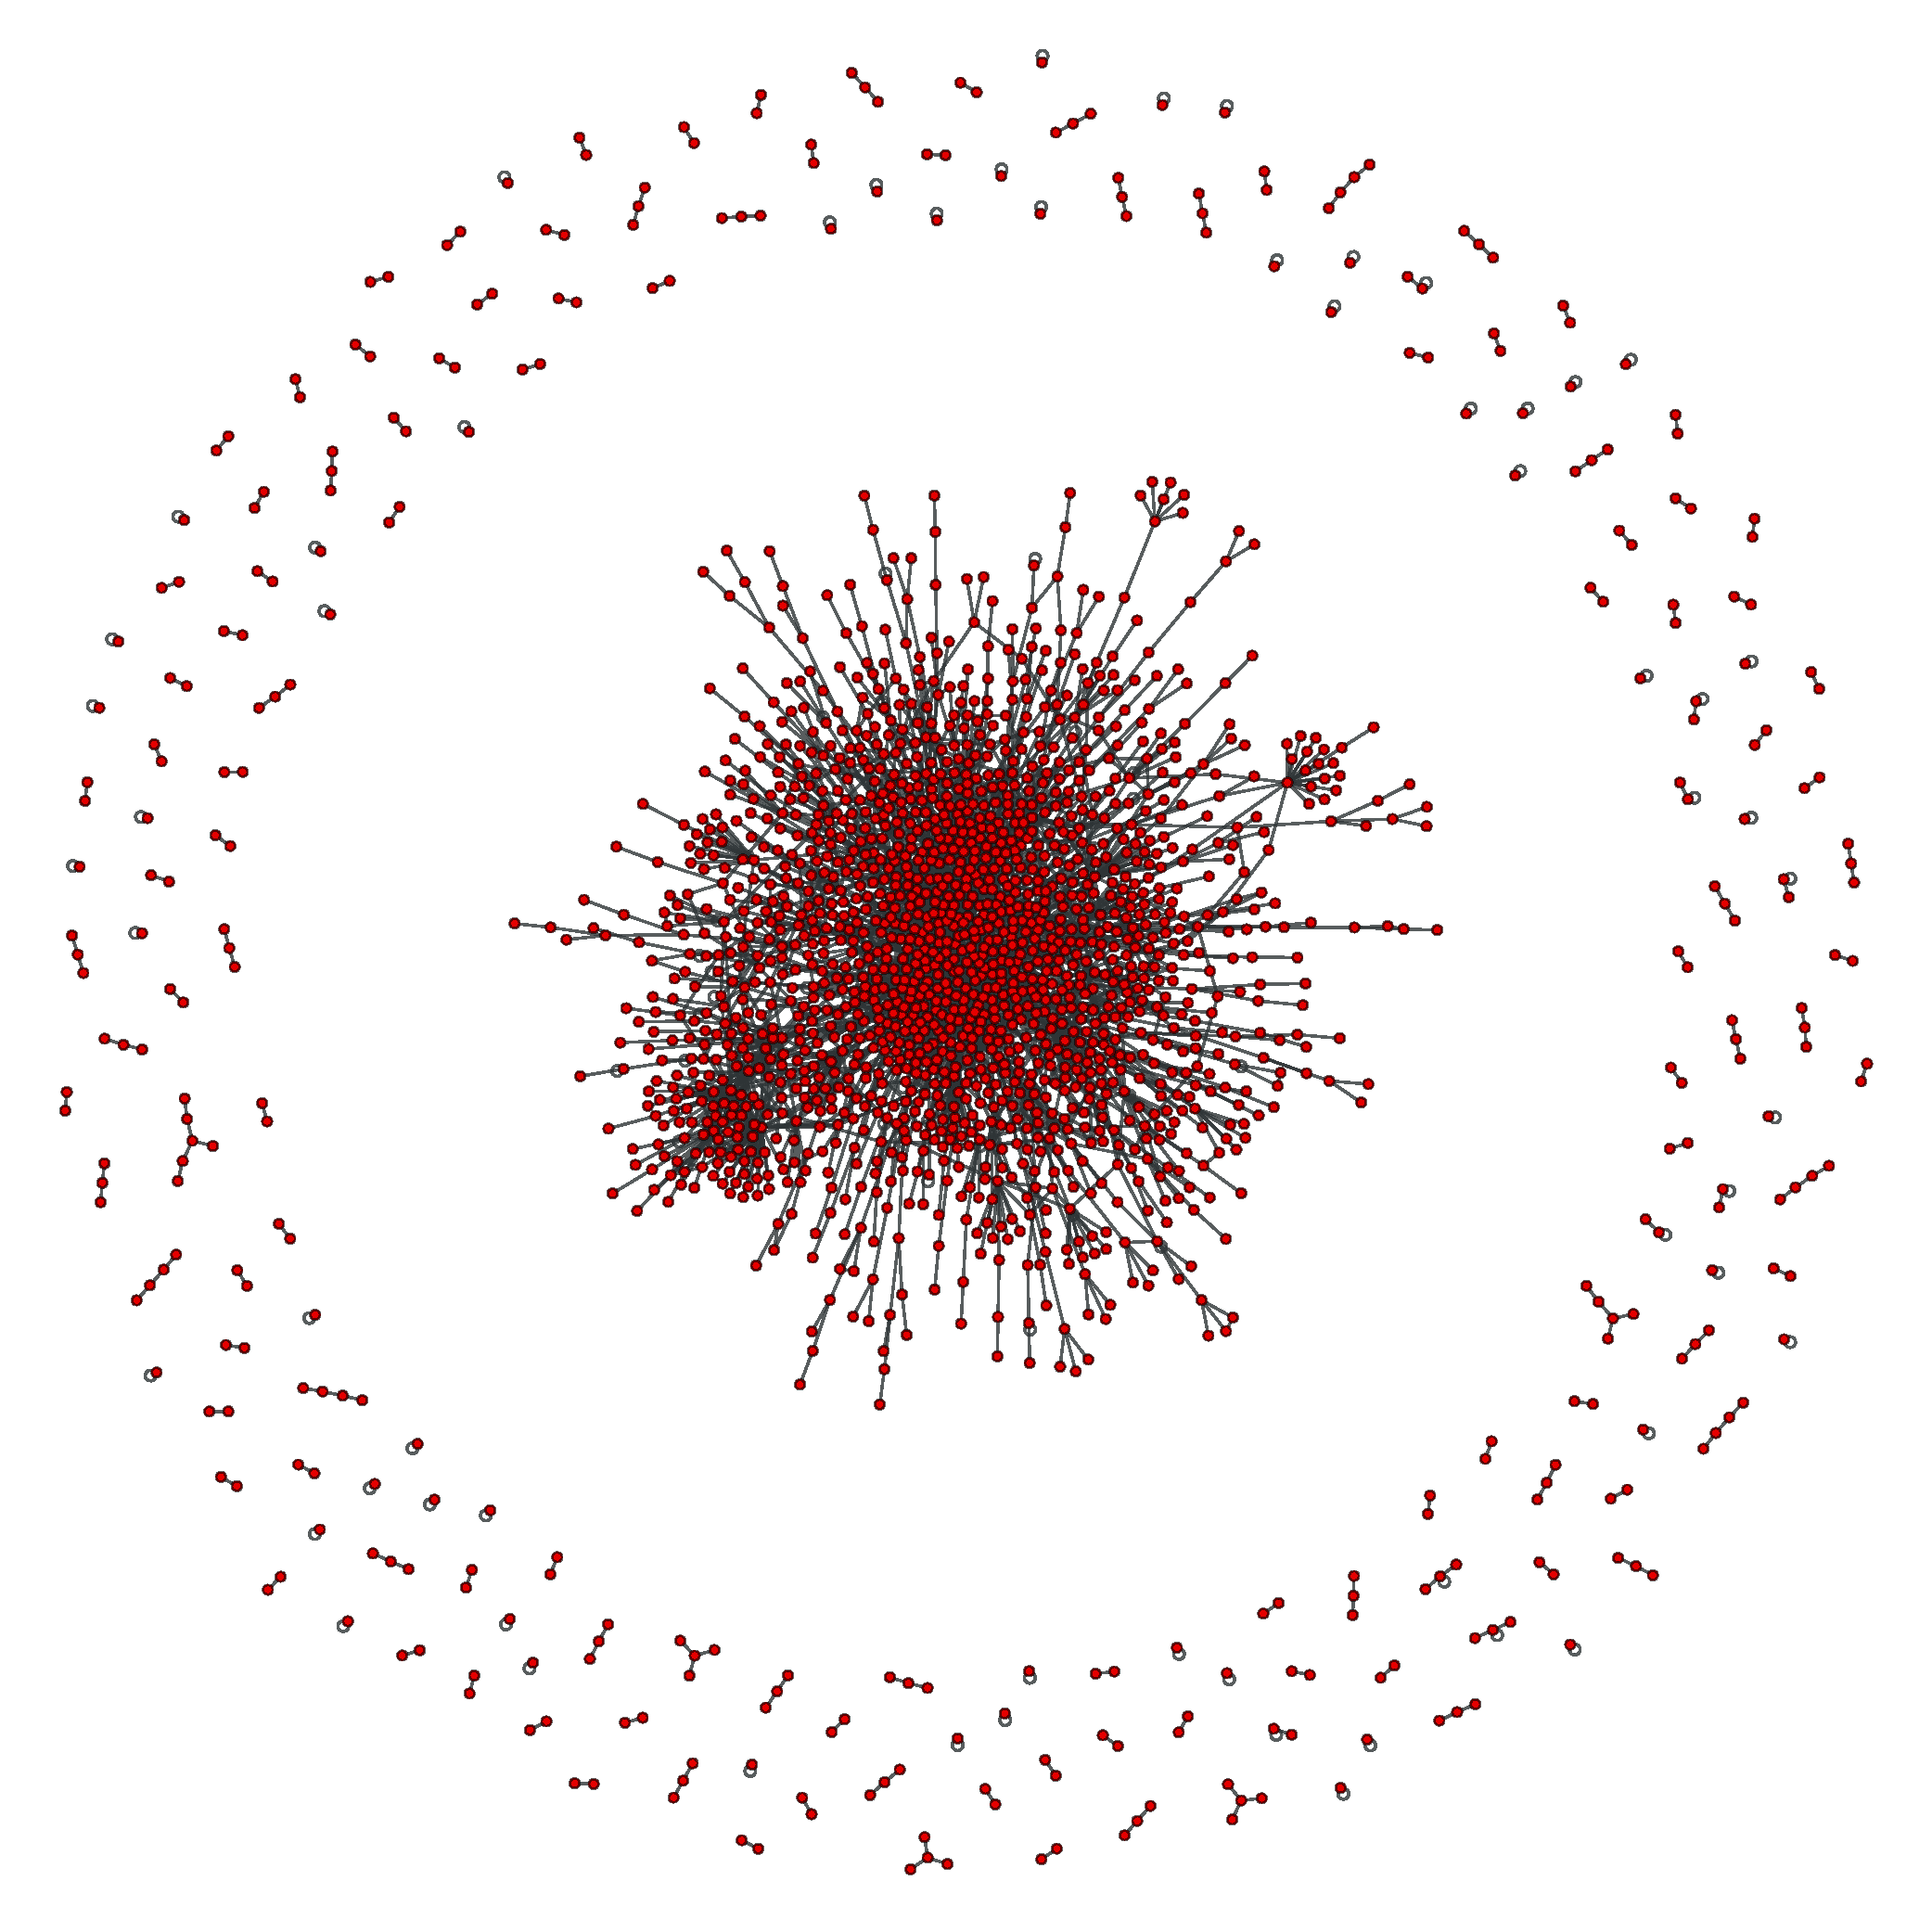
\includegraphics[width=\textwidth]{./schemes/yeast_Y2H-txt.pdf}
        \caption{\label{fig:y2h} Y2H}
    \end{subfigure}
    \\
    \begin{subfigure}[b]{0.4\columnwidth}
        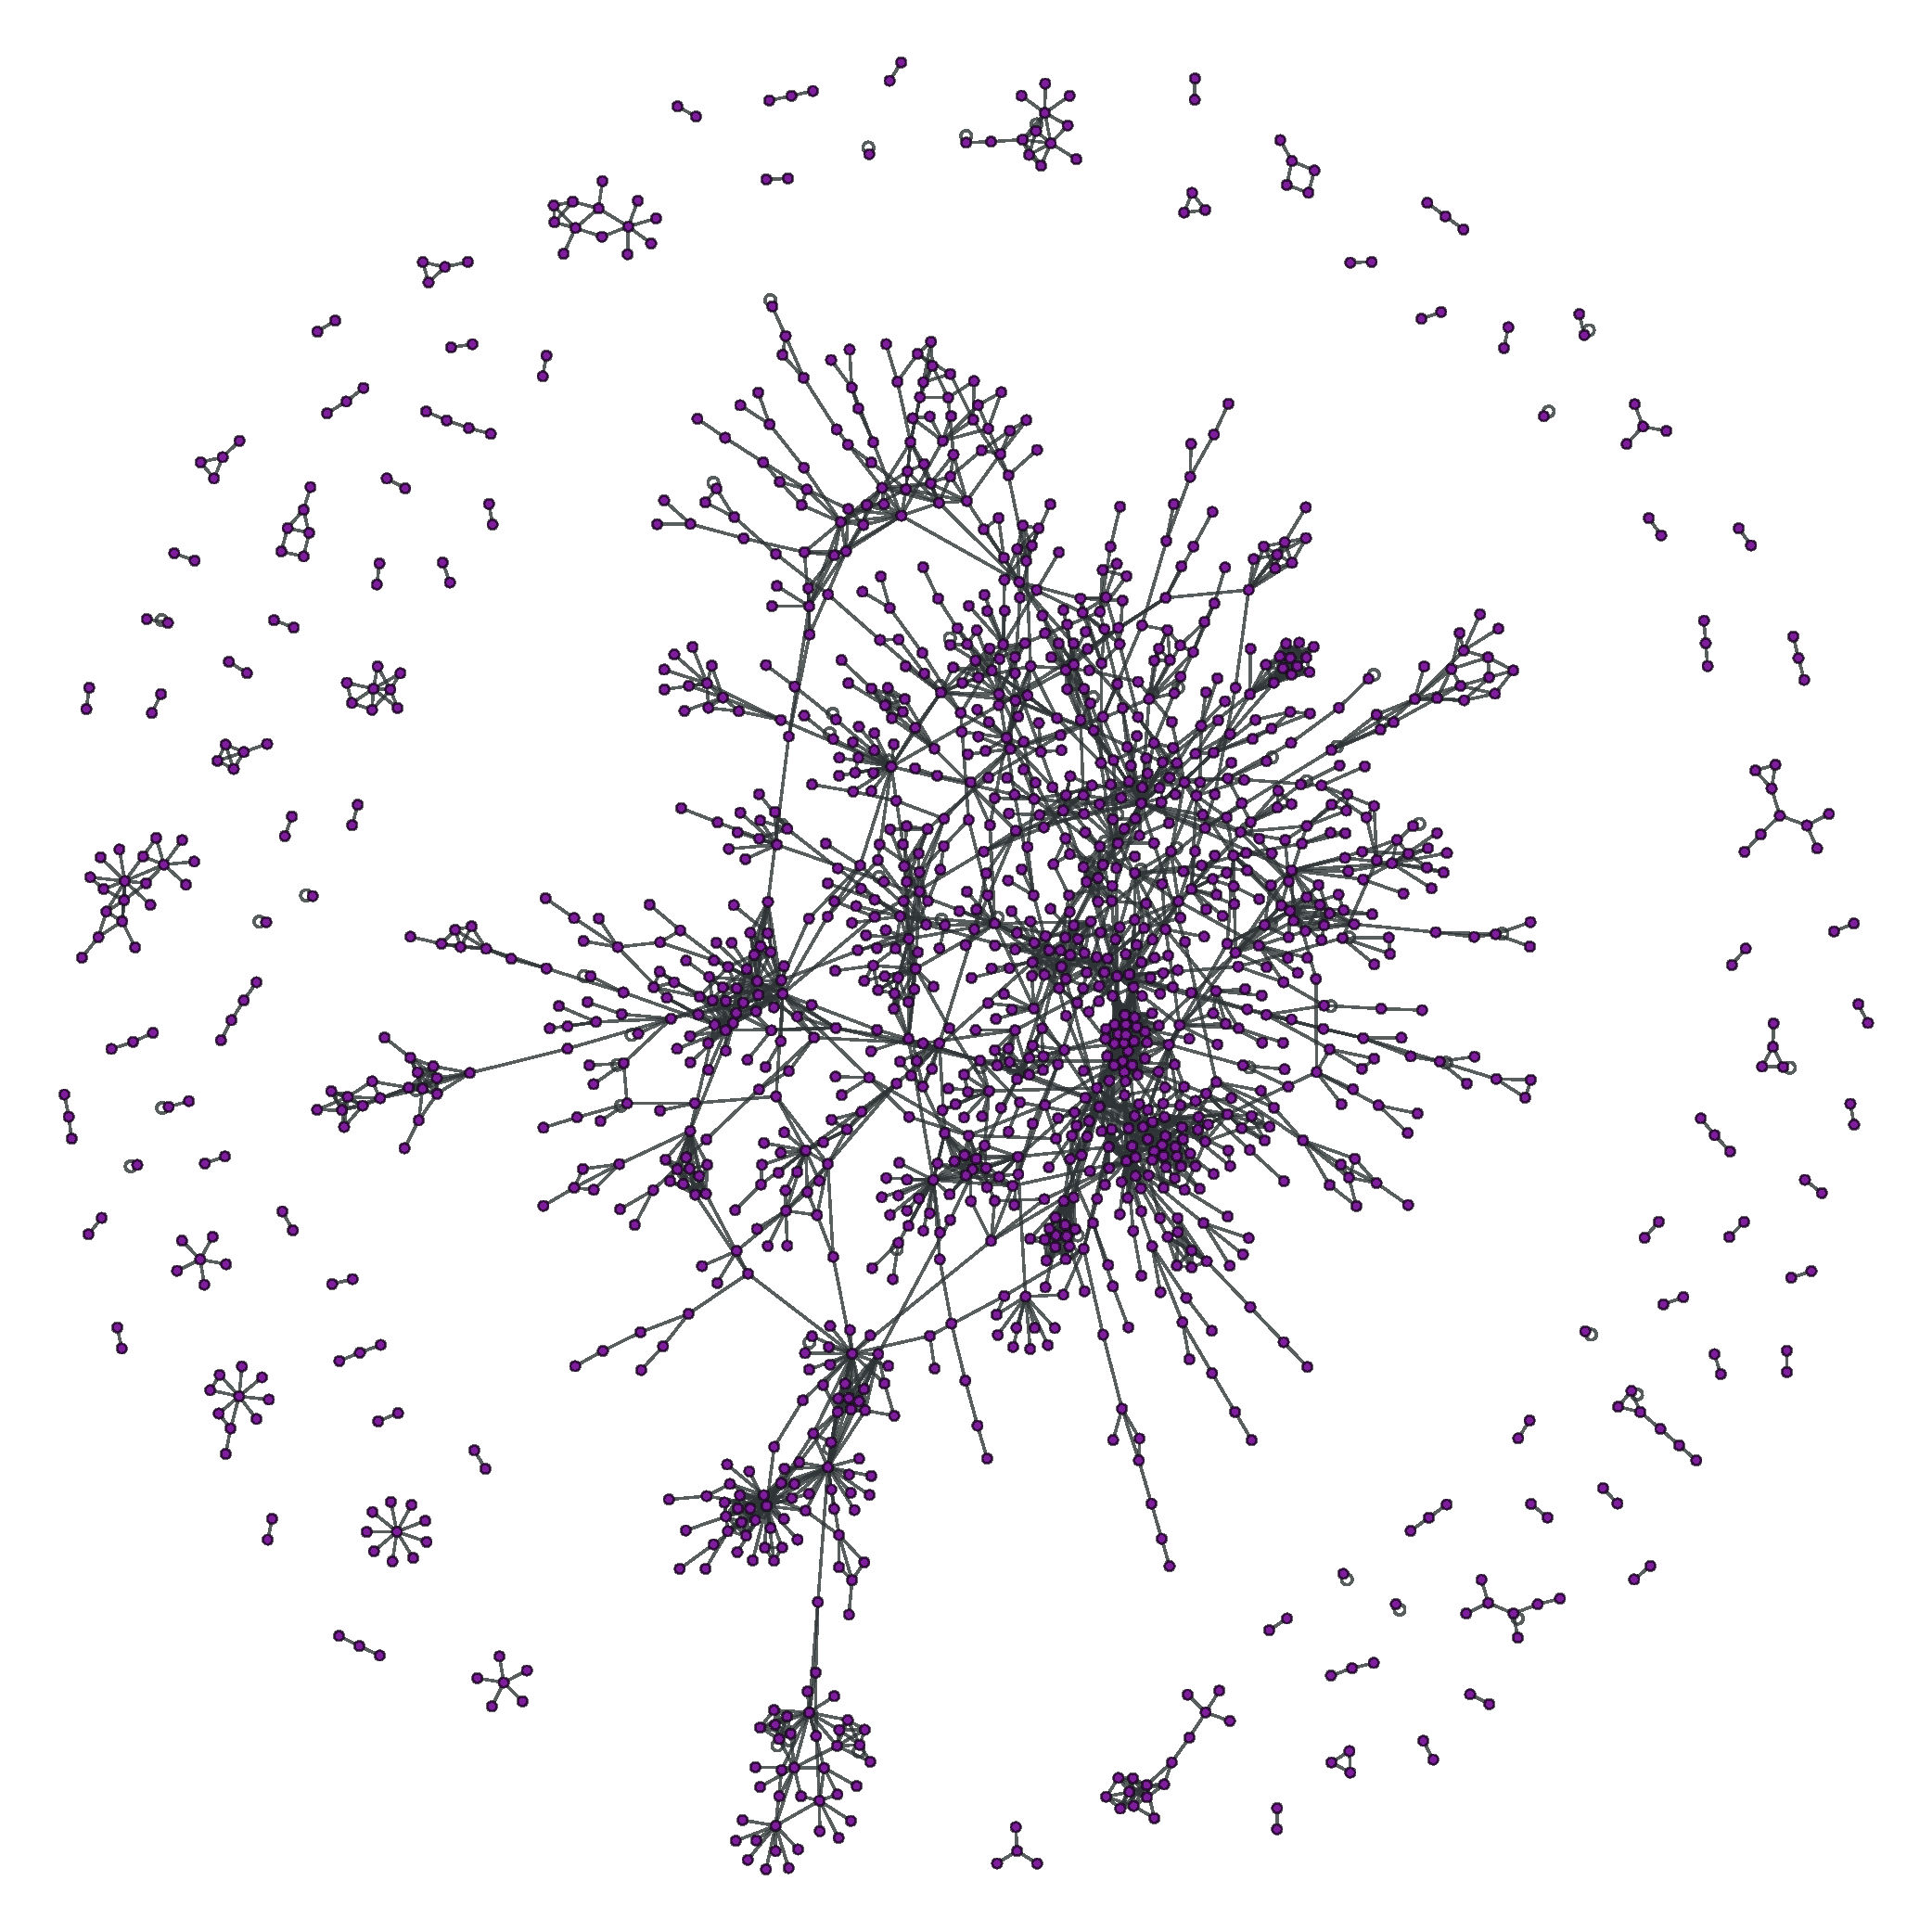
\includegraphics[width=\textwidth]{./schemes/yeast_LIT-txt.pdf}
        \caption{\label{fig:LIT}LIT}
    \end{subfigure}
    \begin{subfigure}[b]{0.4\columnwidth}
        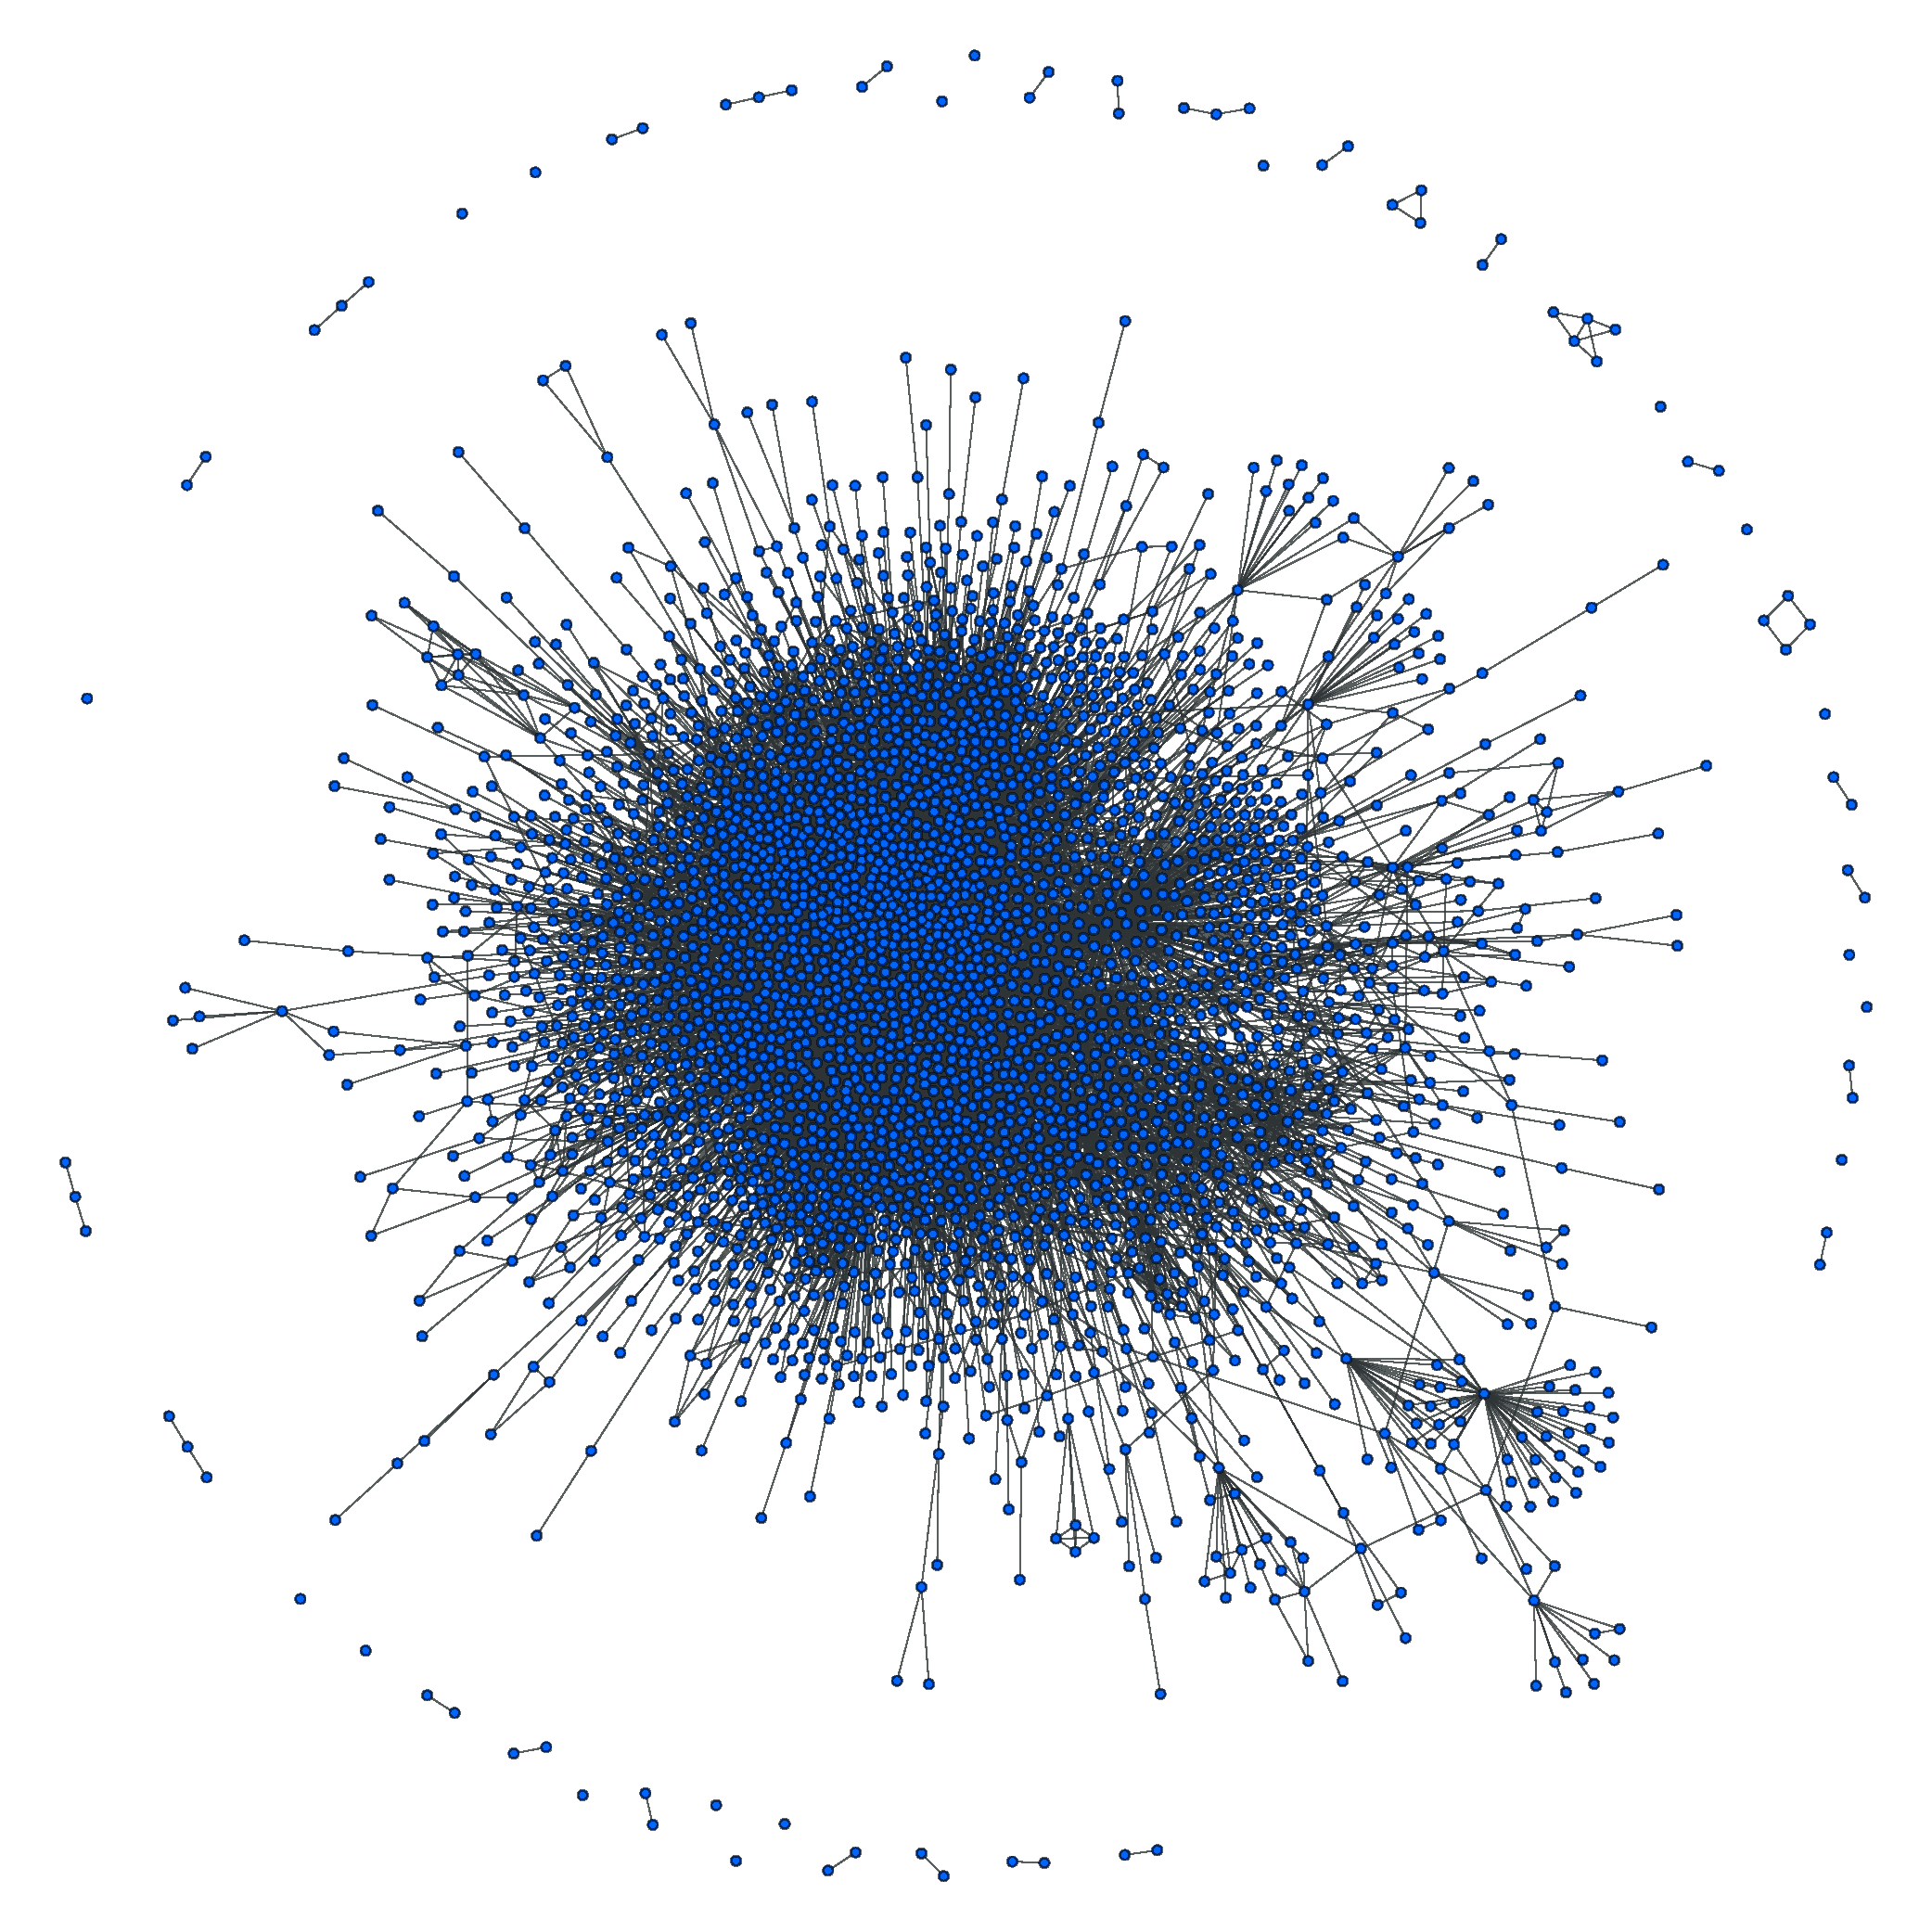
\includegraphics[width=\textwidth]{./schemes/yeast_LIT_Reguly-gml.pdf}
        \caption{\label{fig:LITR}LIT\_Reguly}
    \end{subfigure}
    \caption{\label{grafos} Esquematizaci\'on de los grafos de cada 
    red estudiada.}
\end{figure}

La tabla \ref{tab:obs} muestra un resumen de los observables estad\'isticos desprendidos de las propiedades topol\'ogicas de las redes. Por otro lado, la tabla \ref{tab:overlap} muestra la covertura entre cada par de redes. 

Es importante notar que debido a las diversas t\'ecnicas de construcci\'on de las redes, estas presentan diferencias significativas entre sus observables, como por ejemplo, no es extraño que la red AP-MS sea la que presenta mayor clusterizaci\'on y grado medio debido a que sus enlaces est\'an formados a partir de co-pertenencia a complejos proteicos, mientras que, por ejemplo, Y2H da cuenta de interacciones binarias/f\'isicas entre las proteinas. Adem\'as a partir de la tabla \ref{tab:overlap} se puede ver que las proteinas (nodos) en la red LIT, est\'an totalmente cubiertas por la red LIT\_Reguly, sin embargo esta \'ultima s\'olo cubre un 5\% de los enlaces de la red LIT.



\begin{table}[!ht]
    \centering
    \caption{\label{tab:obs}Observables para las cuatro redes de interacci\'on proteica de levadura.}
    {\scriptsize
    \begin{tabularx}{1\columnwidth}{XlX|XccccX}
        \hline\hline
        &\multirow{2}{*}{Observables}        &&& \multirow{2}{*}{AP-MS} & \multirow{2}{*}{LIT} & \multirow{2}{*}{Y2H} & \multirow{2}{*}{LIT\_Reguly} &\\ 
        &&&&&&\\
        \hline
        &N$^o$ nodos $N$    &&& 1622 & 1536 & 2018 &  3307 &\\
        &N$^o$ enlaces $L$  &&& 9070 & 2925 & 2930 & 11334 &\\
        &Densidad           &&& 0.0068 & 0.0024 & 0.0014 & 0.0020&\\
        &Diametro           &&& 15 & 19 & 14 & 12\\
        \hline
        &Grado $k$&&&\\
  %      \hline
        &\quad medio  $\mean{k}$     &&& 11.18 & 3.80& 2.93 & 6.85 &\\
        &\quad maximo $\max(\{k\})$  &&& 127  & 40   & 91 & 318&\\ 
        &\quad minimo $\min(\{k\})$  &&& 1    & 1    & 1 & 0&\\ 
        \hline
        &Coeficiente de Clusterizaci\'on&&&\\
        \hline
        &\quad medio/local $\mean{C}$               &&& 0.0710 & 0.4556 & 0.0970 & 0.3583&\\
        &\quad triangular/global $C_\bigtriangleup$ &&& 0.6185 & 0.3461 & 0.0236 & 0.1241&\\
        \hline\hline
    \end{tabularx}
    }
\end{table}

\begin{table}[!ht]
    \centering
    \caption{\label{tab:overlap}Observables para las tres redes de interacci\'on prote\'ica de levadura.}
    {\scriptsize
    \begin{tabularx}{.6\columnwidth}{XccccX}
        \hline\hline
        &AP-MS & 0.44 & 0.57 & 0.89 &\\
        &0.35& Y2H &0.36 & 0.66 &\\
        &0.60&0.48& LIT & 1.00 &\\
        &0.43&0.40& 0.46& LIT\_Reguly&\\
        \hline\hline
    \end{tabularx}
    }
\end{table}

%
%
%No es de extra\~nar que, a pesar de que estas 3 redes de proteinas 
%pertenecen al mismo organismo (\textit{Saccharomyces cerevisiae}),
%estas son distintas topol\'ogicamente debido a la manera en que son armadas.
%La red AP-MS muestra la formaci\'on de varios grupos/clusters muy densos que corresponden
%a los complejos proteicos purificados, esto se ve reflejado en los observables de la tabla \ref{tab:obs}
%en que, salvo el di\'ametro, presenta mayores valores que el resto de las redes. 
%Cabe observar que la red de literatura LIT presenta el mayor di\'ametro, sin embargo es la con 
%menor grado m\'aximo (por lo que pareciera capaz de relacionar m\'as interacciones entre clusters), debido a la compilaci\'on
%de un gran n\'umero de trabajos, pero tiene menor detalle de las interacciones prote\'ina-prote\'ina, debido
%a que en general los trabajos consultados son espec\'ificos y por lo tanto sesgados (hay perdida de informaci\'on las proteinas
%menos estudiadas).
%En particular al observar la clusterizaci\'on es importante diferenciar la clusterizaci\'on media $\mean{C}$ y la 
%clusterizaci\'on triangular $C_\bigtriangleup$. La primera caracteriza la media de la clusterizaci\'on local de cada 
%nodo, es por ello que la red LIT prensenta el mayor valor, debido a que, como mencionamos antes, compila
%trabajos detallados que dan cuenta de peque\~nos clusters. Tanto la red AP-MS y, a\'un m\'as, la red Y2H diluyen
%su clusterizaci\'on debido a un gran n\'umero de \textit{peque\~nas interacciones aisladas}. Por otro lado
%el coeficiente $C_\bigtriangleup$ es una medida m\'as global, ya que no pesa interacciones bin\'arias puras.
%En este \'ultimo caso AP-MS presenta la mayor clusterizaci\'on, mientras que Y2H la menor.
%
%
%\subsection{Coherencia entre las redes}
%
%\begin{figure}[!ht]
%    \centering
%    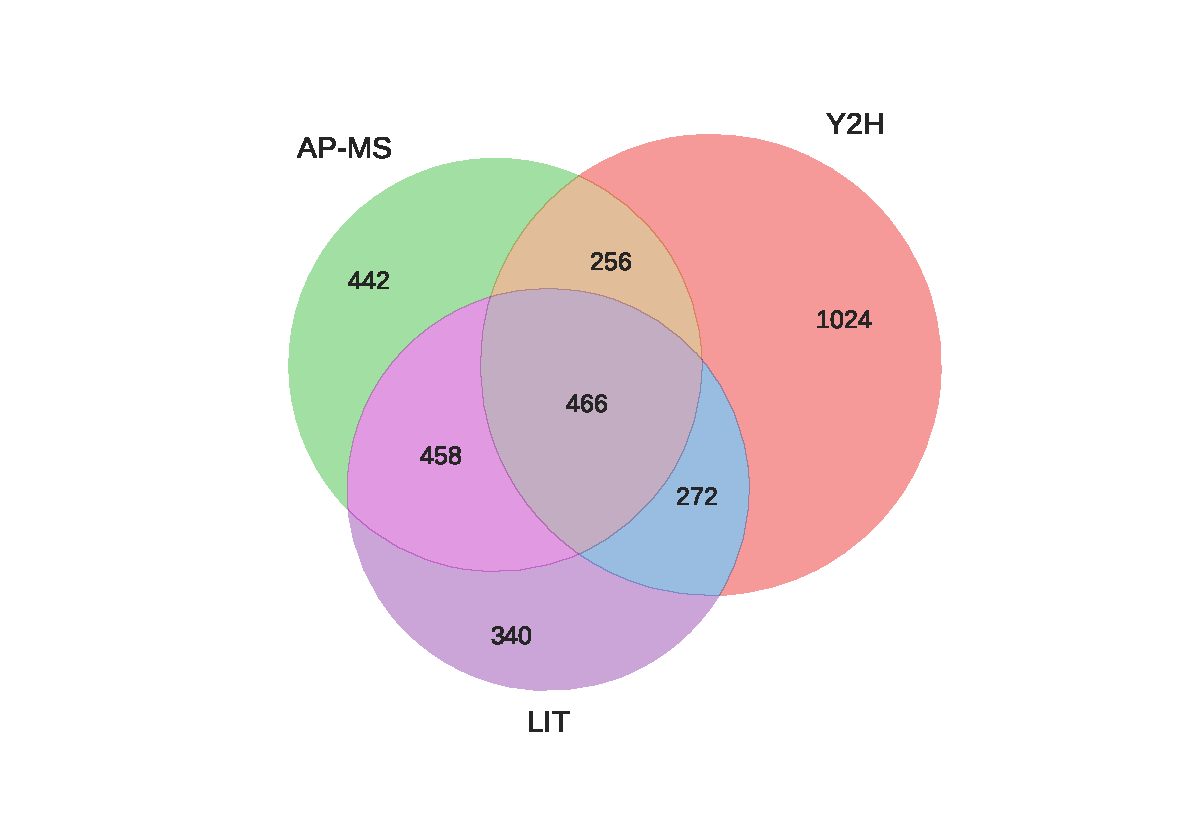
\includegraphics[width=.5\columnwidth]{./schemes/venn_AP-MS-Y2H-LIT_covertura.pdf}
%    \caption{\label{fig:cober} Diagrama de Venn para cobertura entre las tres redes. }
%\end{figure}
%
%
%
%En segundo lugar se analiz\'o la cobertura y coherencia entre las interacci\'ones reportadas
%en las redes. Para ello se realiz\'aron los diagramas de Venn mostrados en la figura \ref{fig:cober}, \ref{fig:venn} y \ref{fig:subgrafos}
%(estos pueden reproducirse con el script \texttt{venn.py} \texttt{venn2.py}). Para analizar la covertura comparamos
%la intersecci\'on de las prote\'inas reportadas en cada caso. En la figura \ref{fig:cober} se muestra
%la cobertura de cada red y la cantidad de proteinas reportadas por m\'as de una red (intersecciones). Es 
%interesante notar que AP-MS y LIT presentan $\sim 60\%$ de cobertura entre ellas y solo un $\sim 27\%$ 
%y un $\sim 22\%$ de las prot\'inas reportadas, respectivamente, son especificas de cada red. Esto se ve contrastado
%con el $\sim 50\%$ de especificidad en la red Y2H. 
%
%
%\vspace{1.5cm}
%\begin{figure}[!ht]
%    \centering
%    \begin{subfigure}[b]{0.48\columnwidth}
%        \centering
%        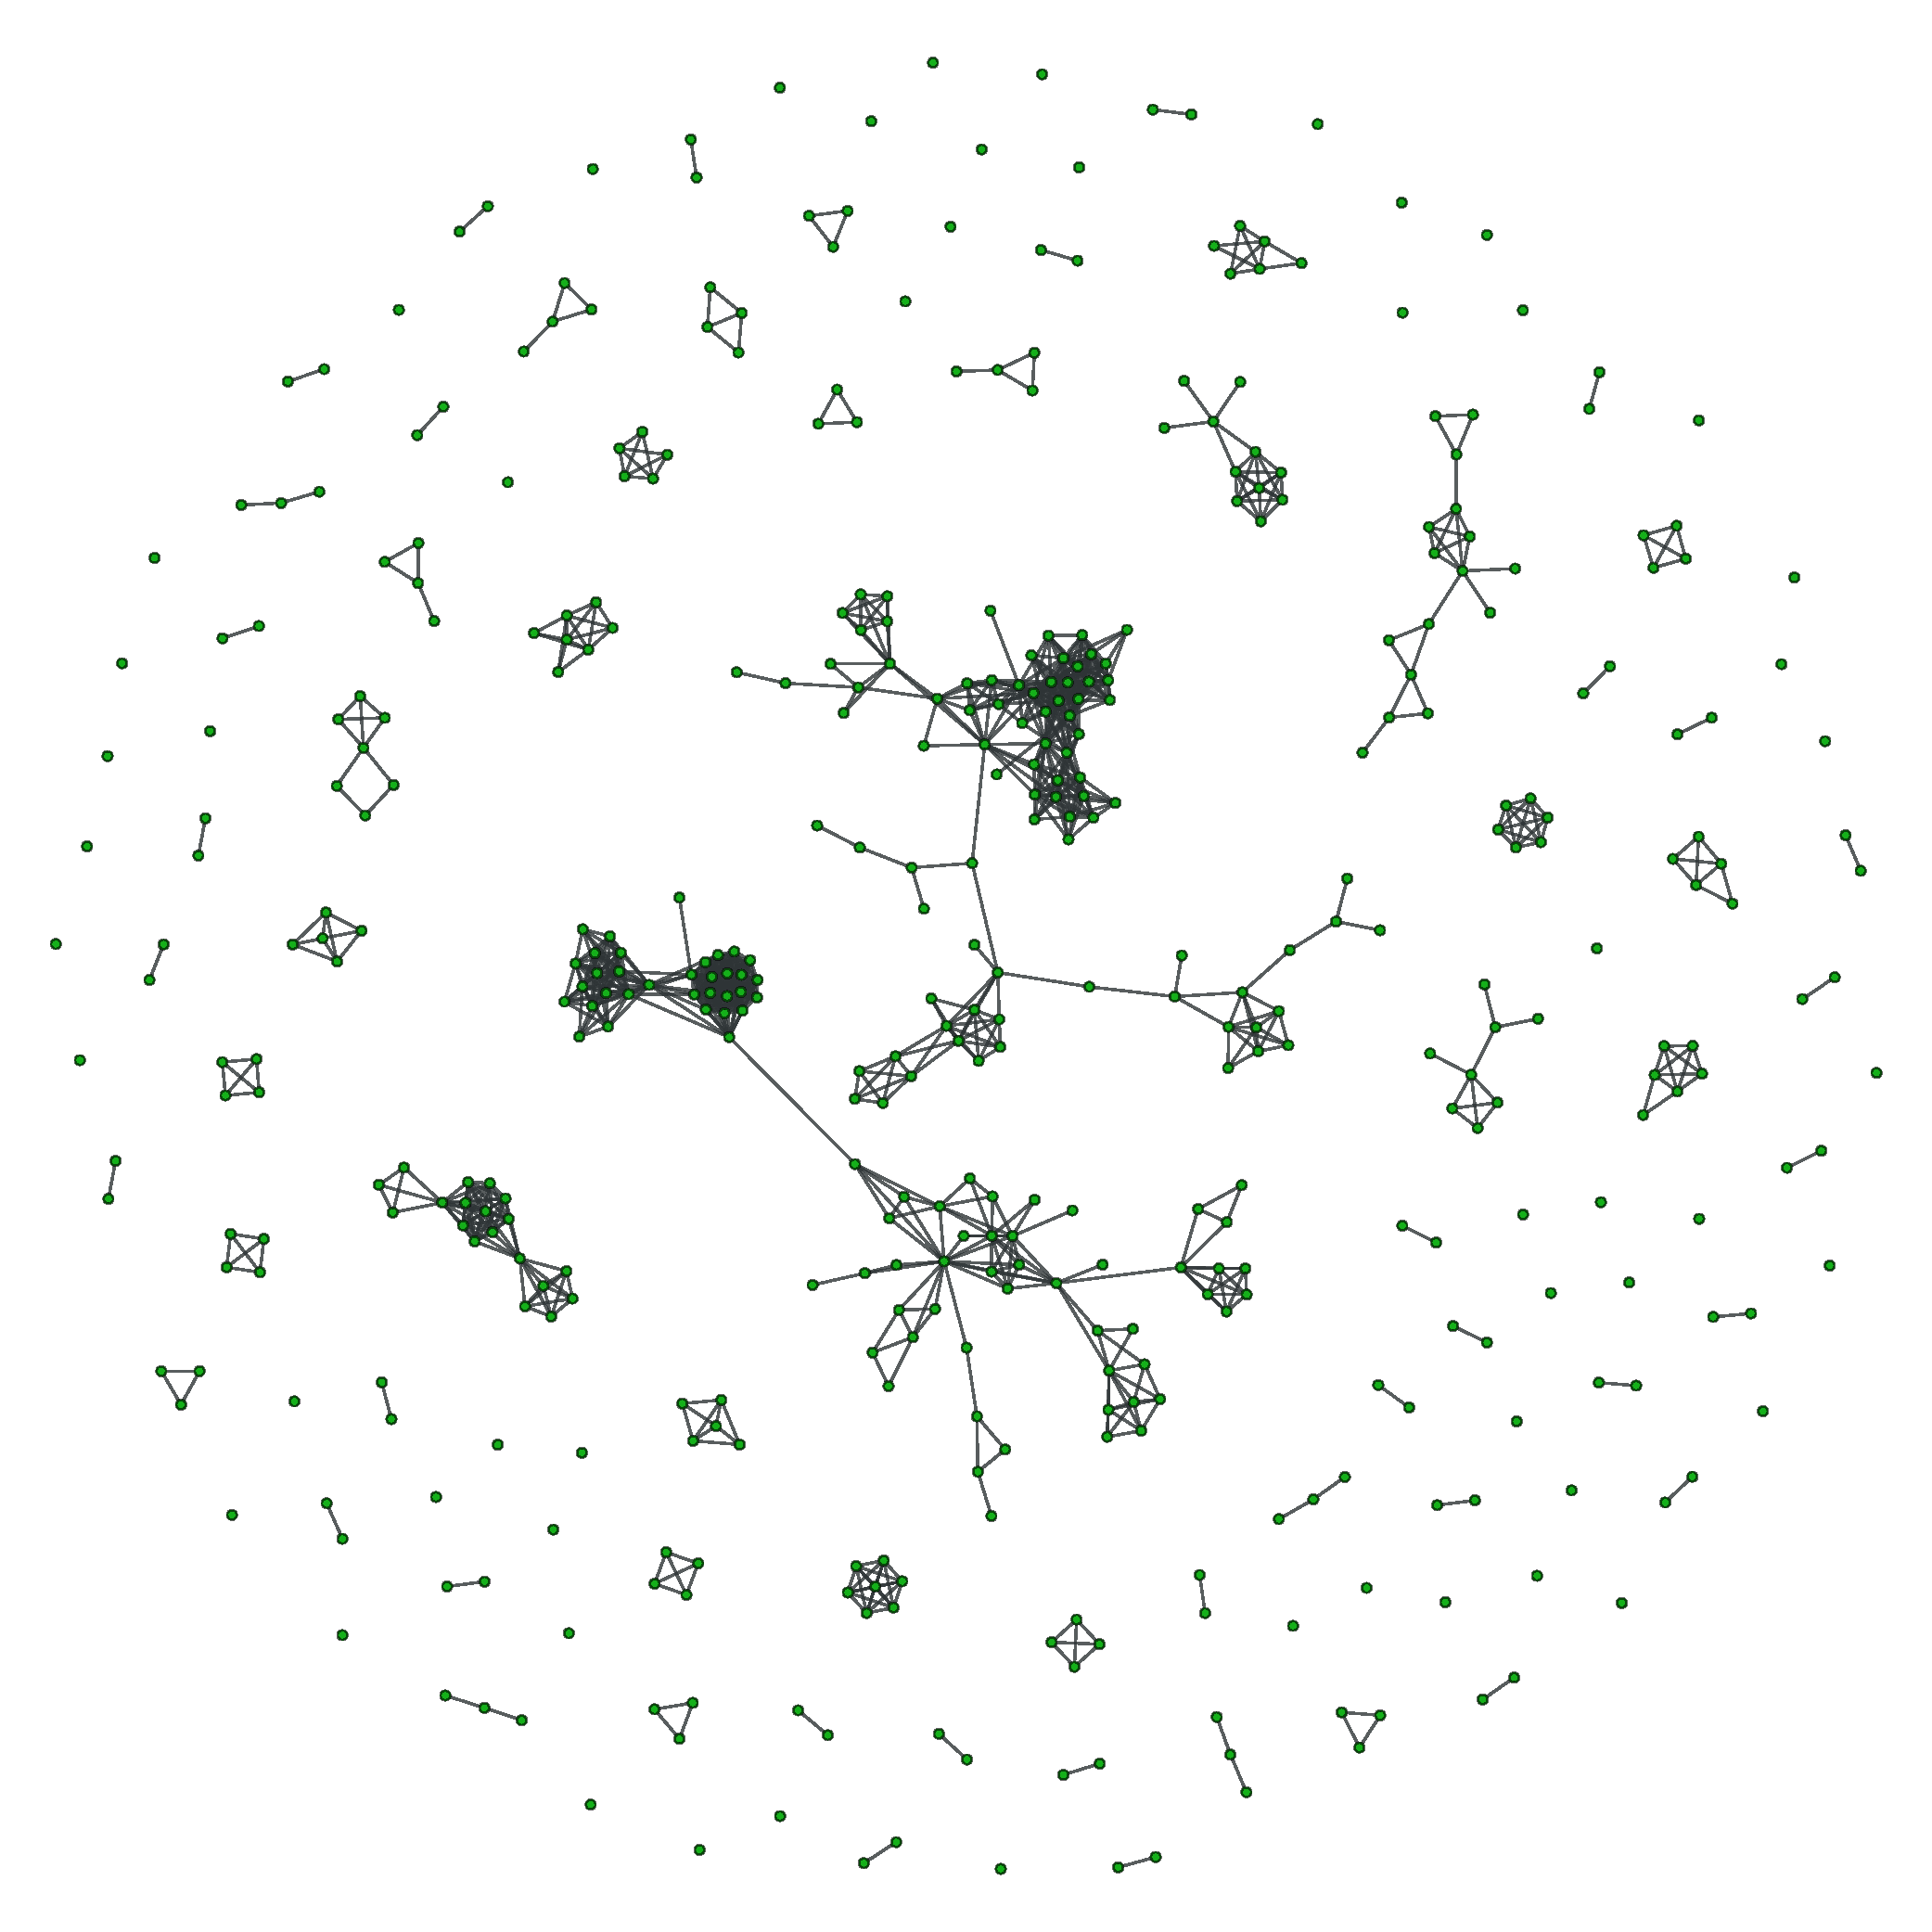
\includegraphics[width=.45\textwidth]{./schemes/subgrafo_AP-MS_all-gml.pdf}
%        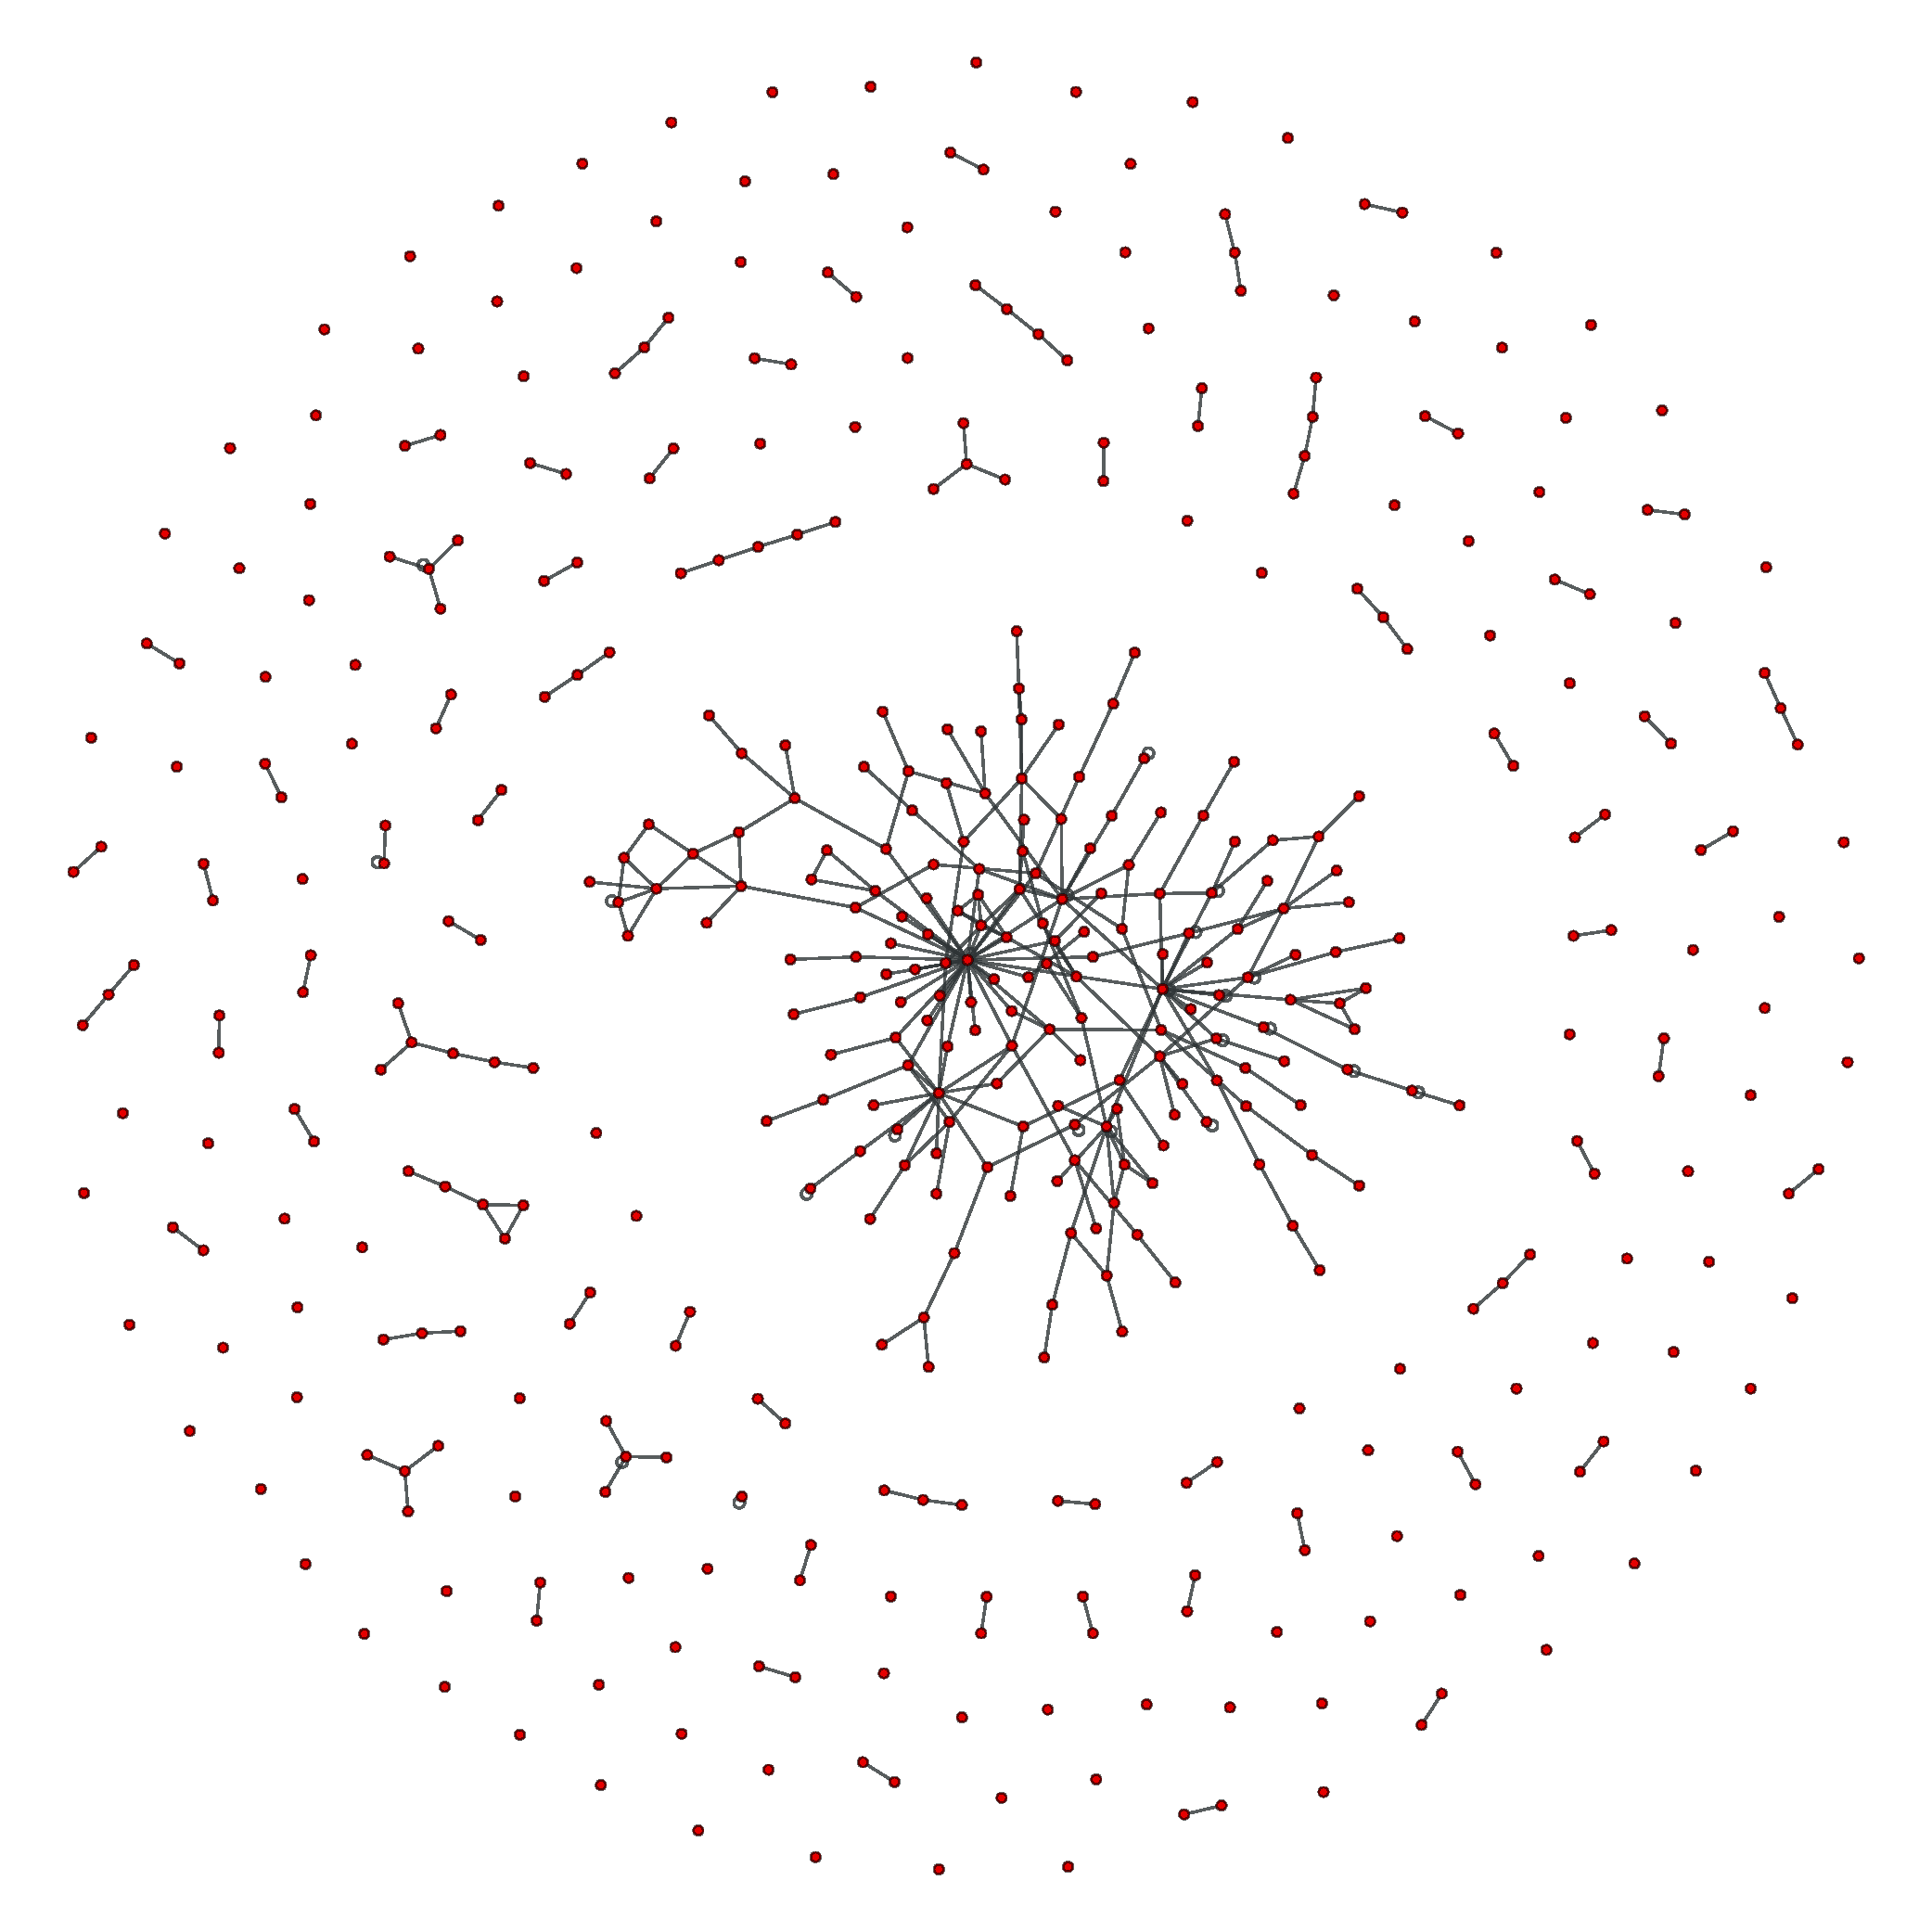
\includegraphics[width=.45\textwidth]{./schemes/subgrafo_Y2H_all-gml.pdf}\\
%        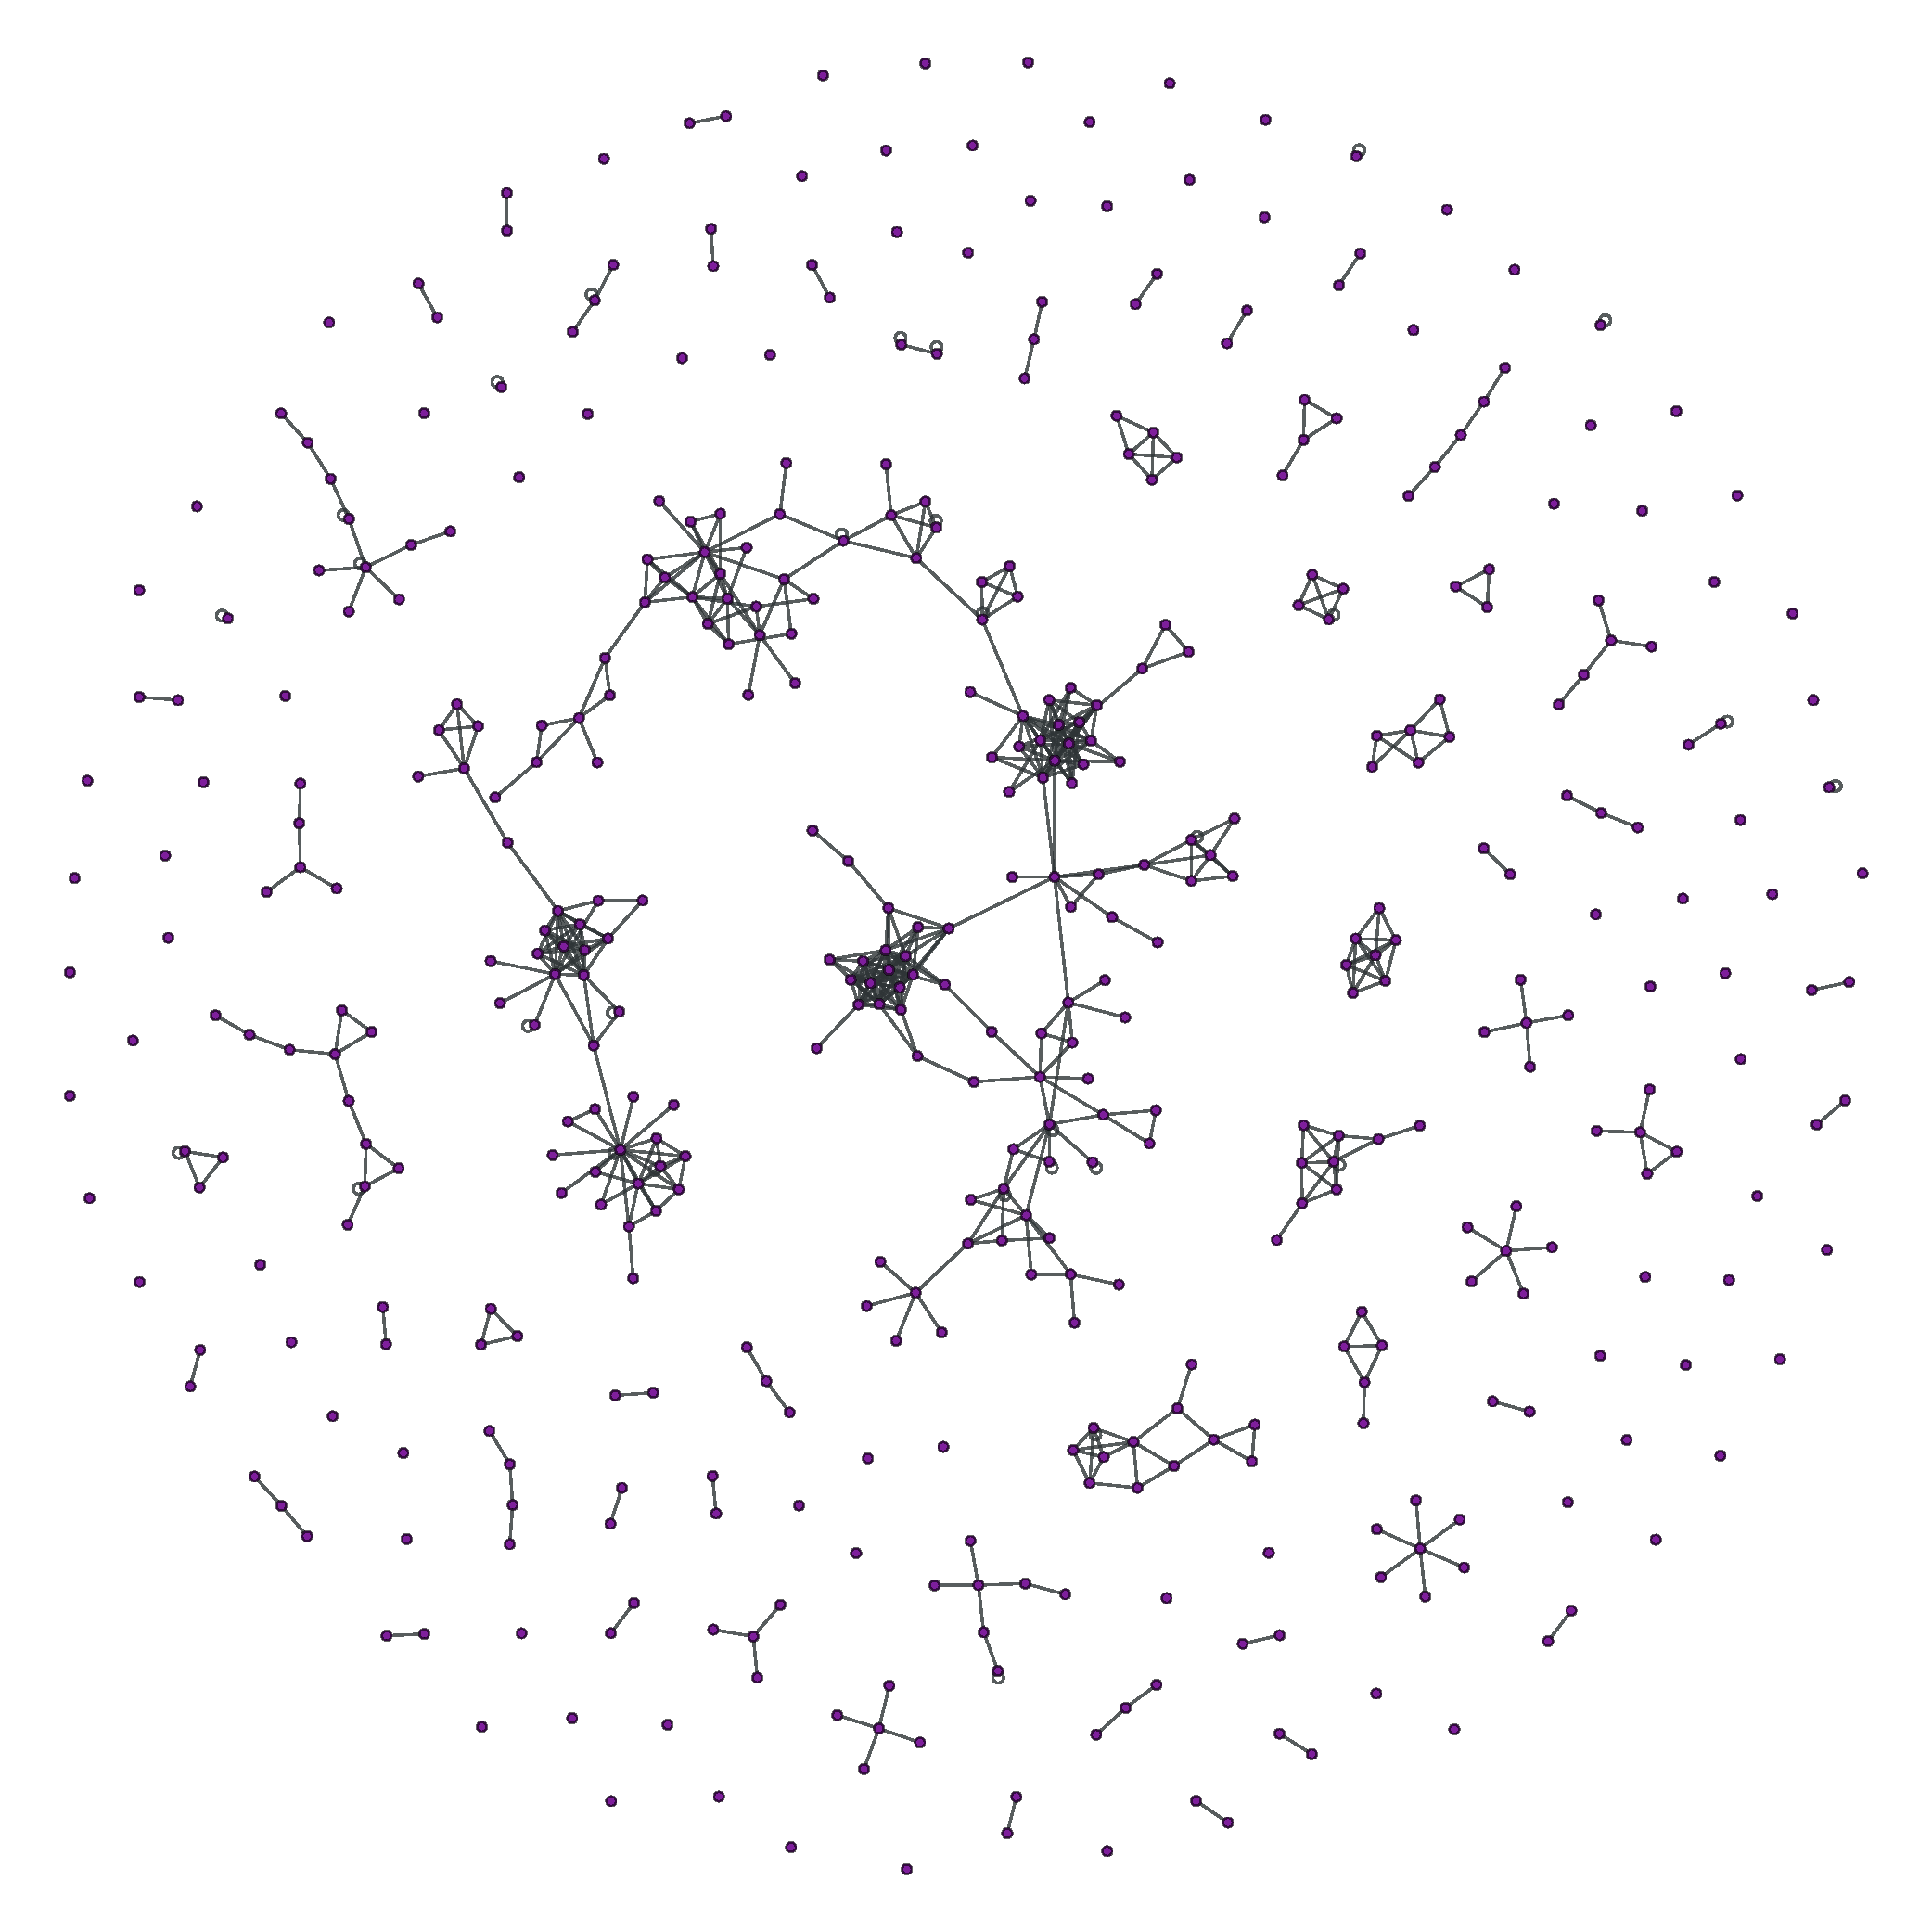
\includegraphics[width=.45\textwidth]{./schemes/subgrafo_LIT_all-gml.pdf}
%        \caption{\label{fig:all} AP-MS/Y2H/LIT}
%    \end{subfigure}
%    \hfill
%    \begin{subfigure}[b]{0.48\columnwidth}
%        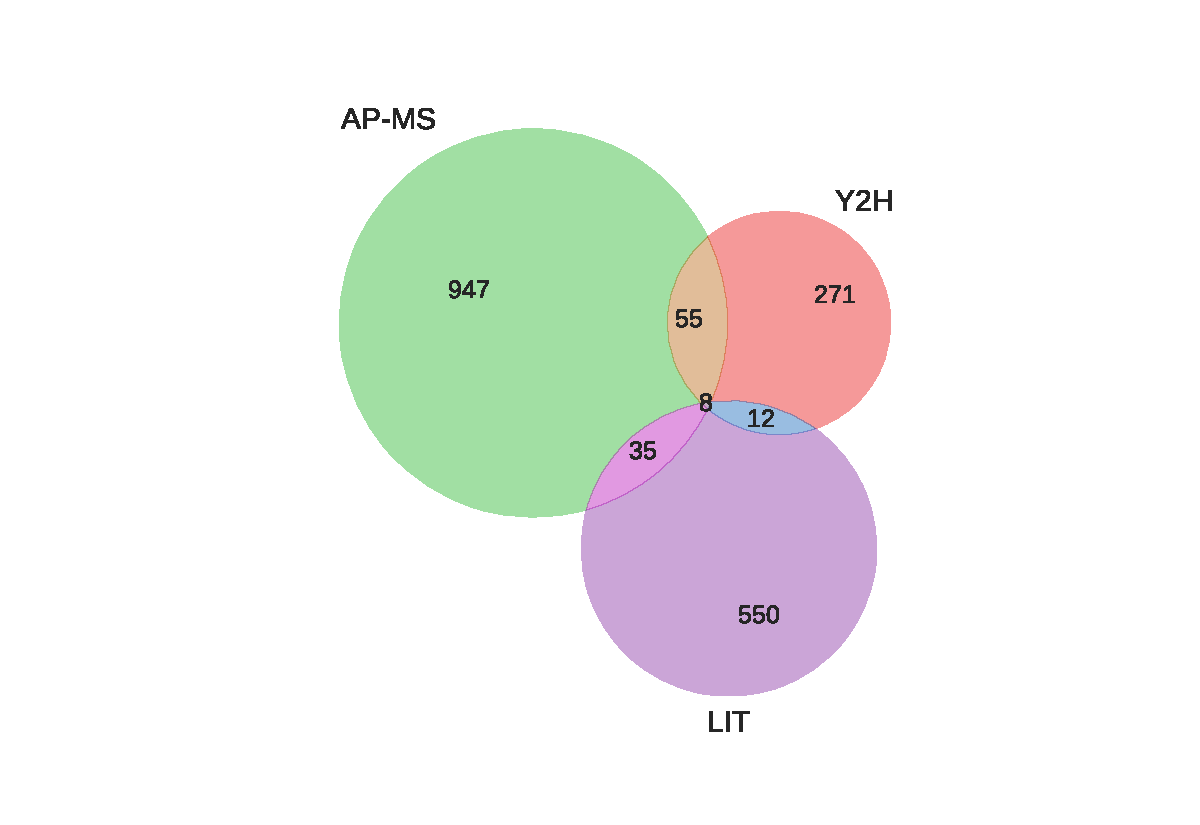
\includegraphics[width=\textwidth]{./schemes/venn_AP-MS-Y2H-LIT_links.pdf}
%        \caption{\label{fig:cohe} Coherencia}
%    \end{subfigure}
%    \caption{\label{fig:venn} Subgrafos inducidos por cobertura de las 3 redes y coherencia de links entre ellas. }
%\end{figure}
%
%\vspace{1.5cm}
%Por otra parte, a partir de la intersecci\'on de las prote\'inas reportadas de las tres redes, se analiza la coherencia
%de los enlaces entre las prote\'inas comunes. De la figura \ref{fig:cohe} se puede observar al alta especificidad
%de cada red respecto al resto (solo 8 links son compartidos por las tres redes). 
%
%
%\begin{figure}[!ht]
%    \centering
%    \begin{subfigure}[b]{0.3\columnwidth}
%        \centering
%        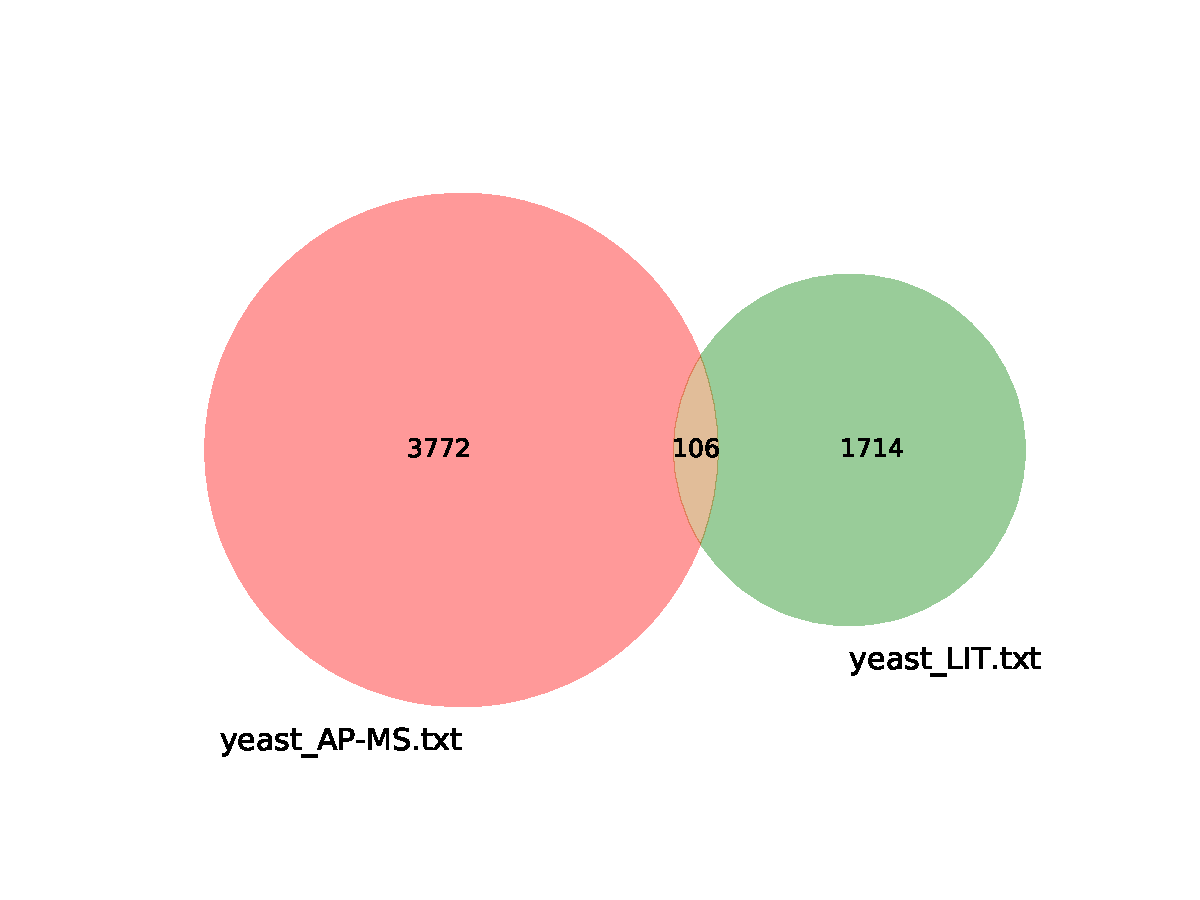
\includegraphics[width=.7\textwidth]{./schemes/venn2_coherence_yeast_AP-MS-yeast_LIT.pdf}\\
%        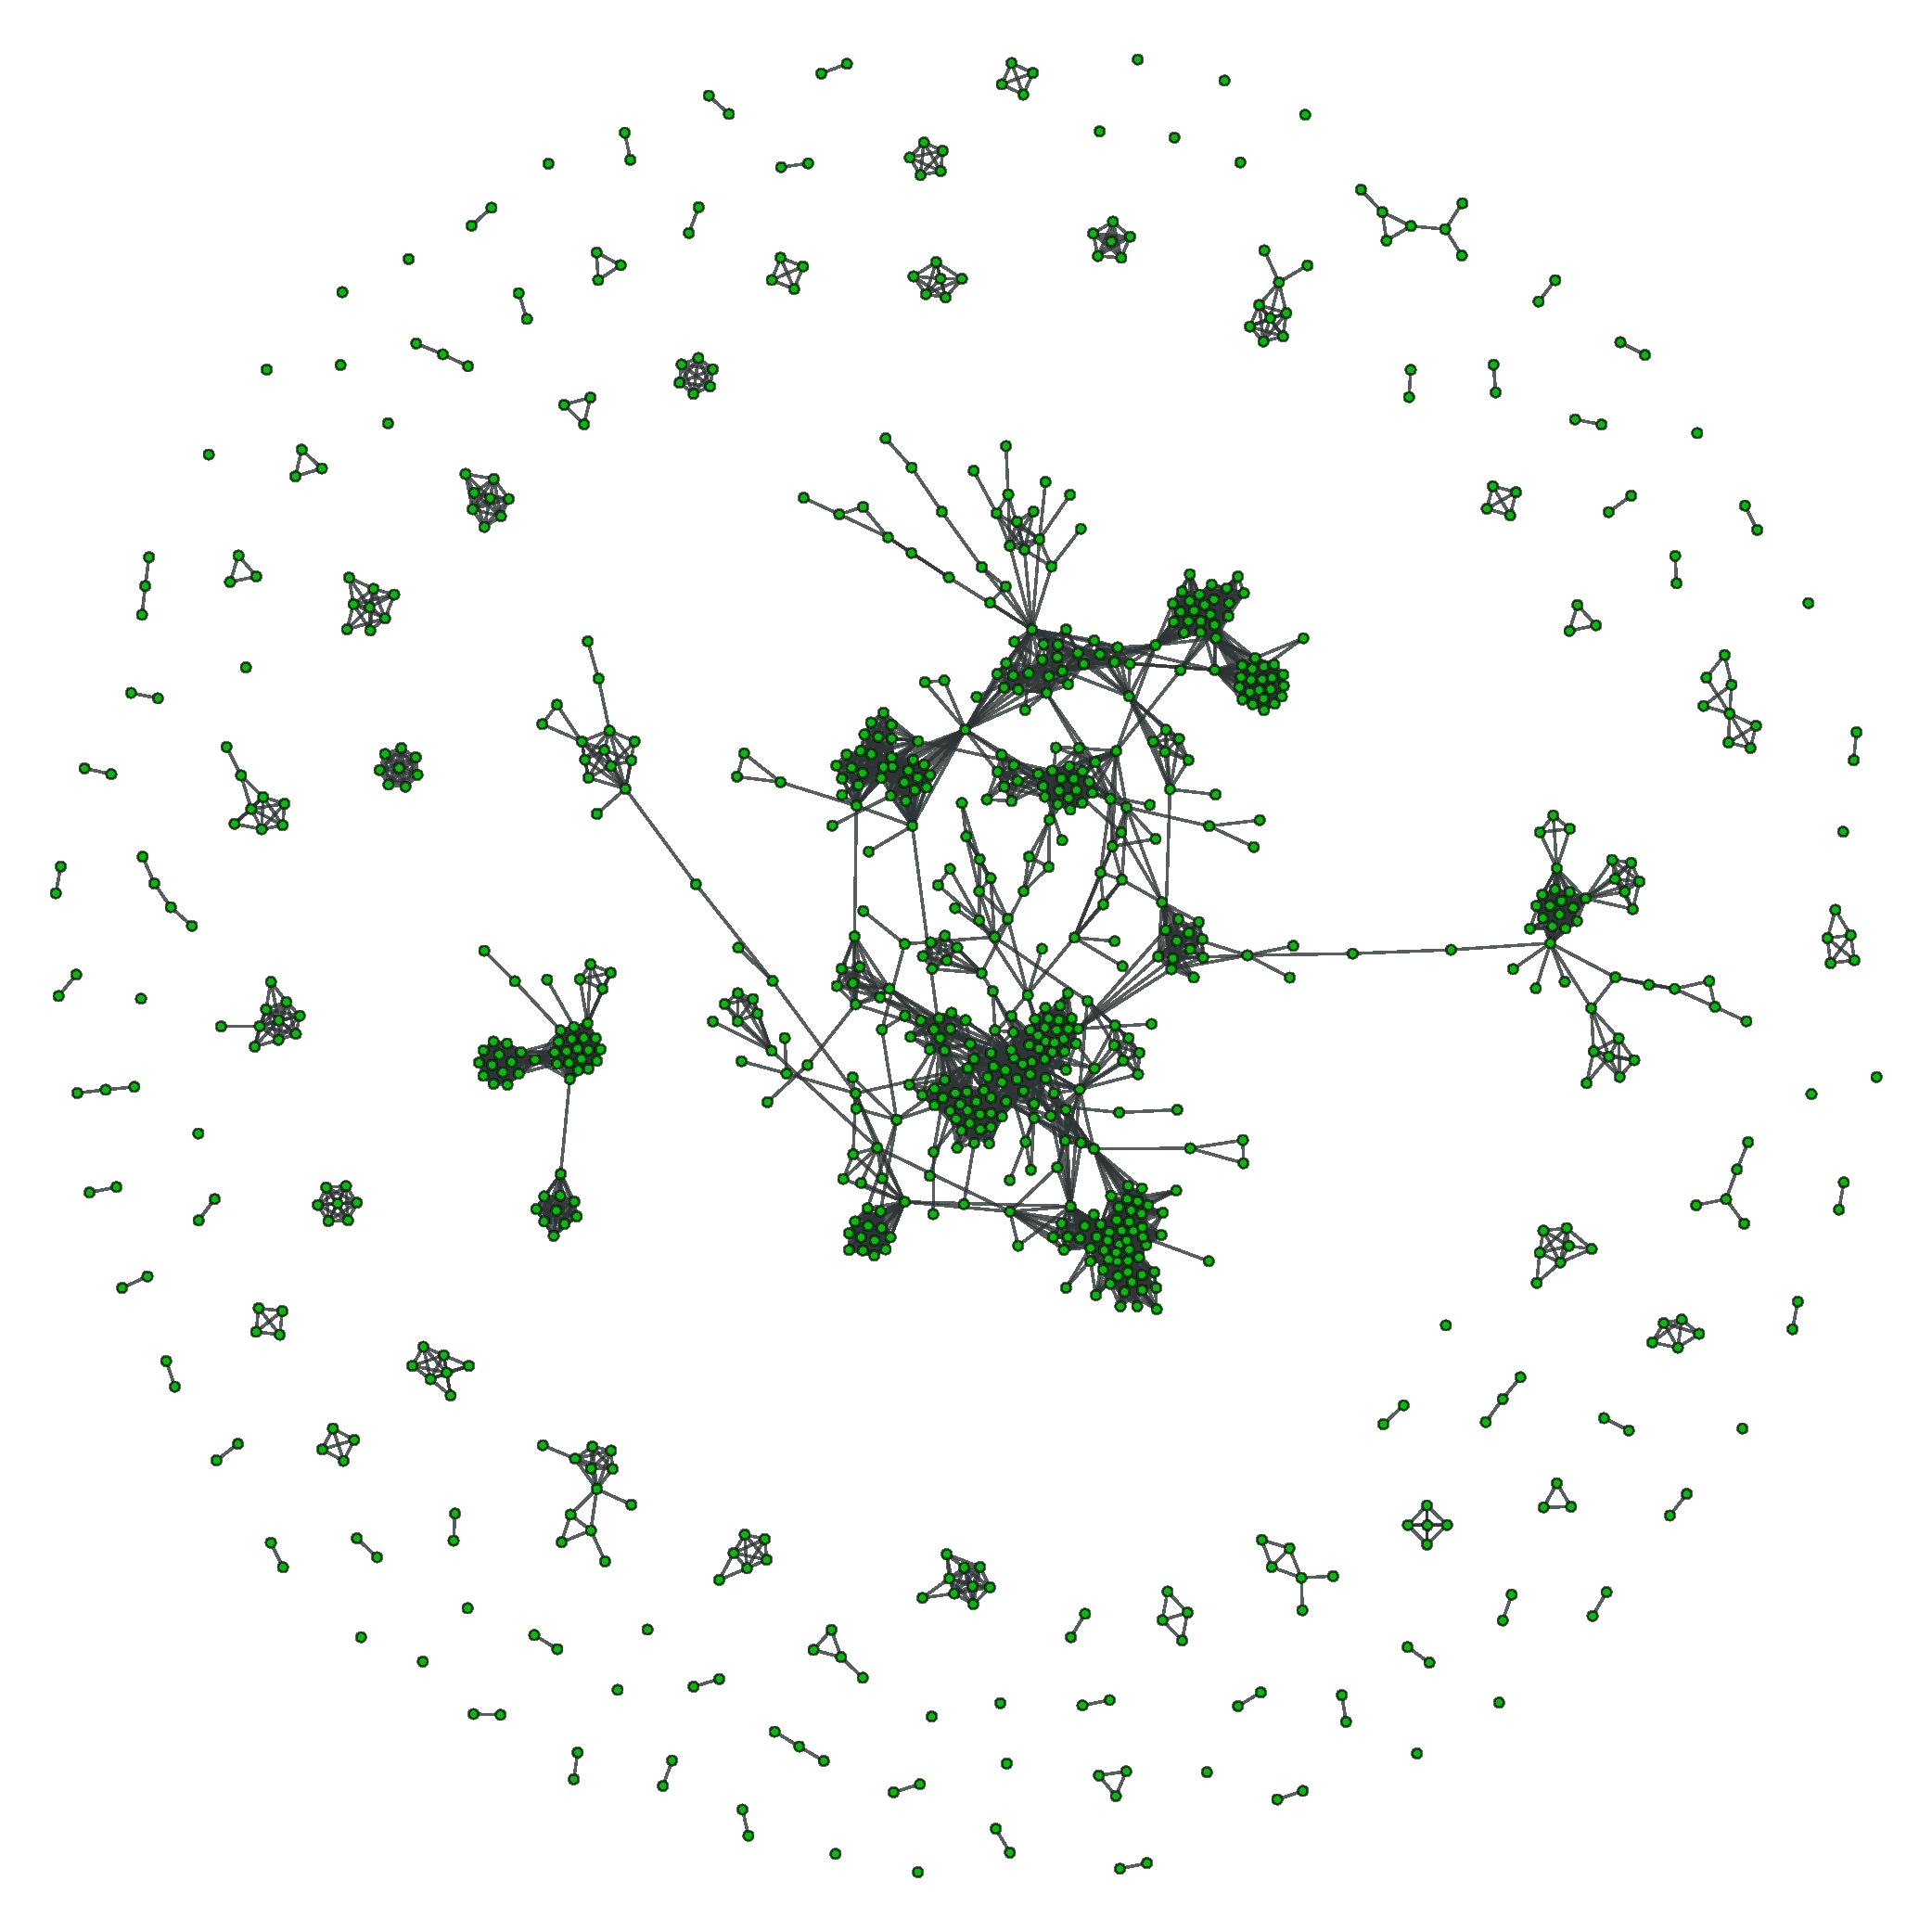
\includegraphics[width=.45\textwidth]{./schemes/subgrafo_APMS_ap_ms_lit-gml.pdf}
%        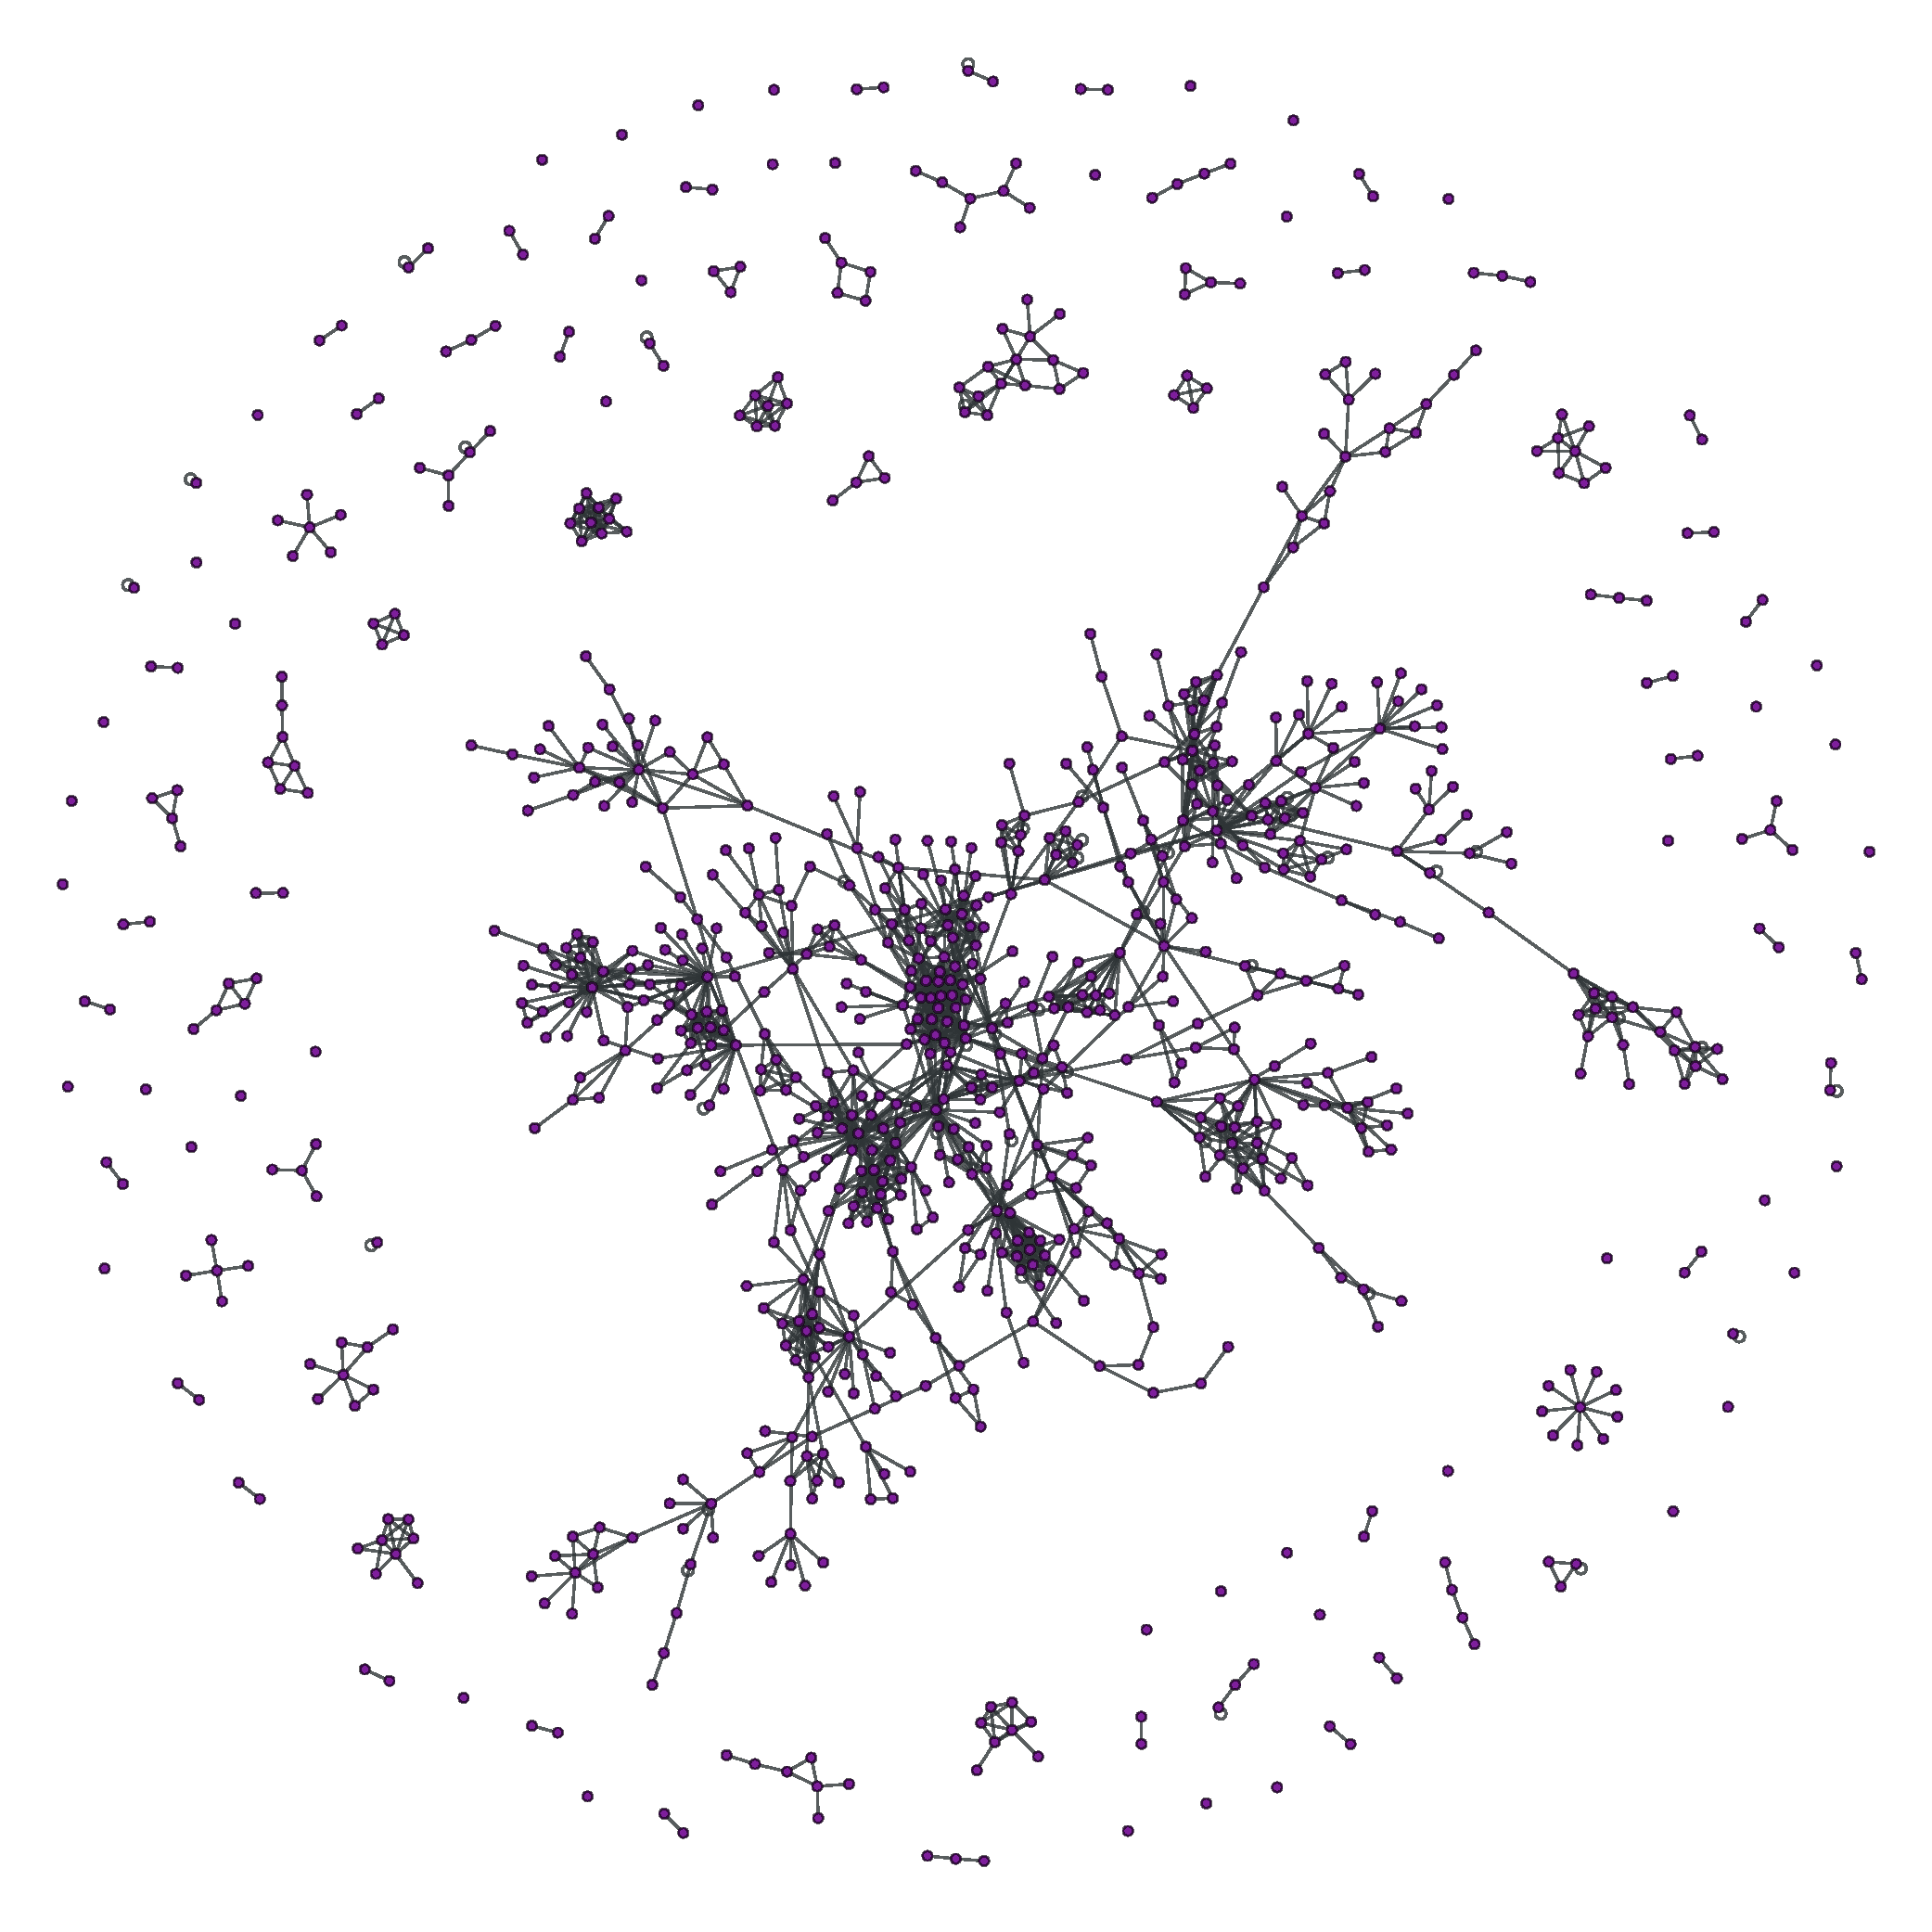
\includegraphics[width=.45\textwidth]{./schemes/subgrafo_LIT_ap_ms_lit-gml.pdf}
%        \caption{\label{fig:apms-lit} AP-MS/LIT}
%    \end{subfigure}
%    \begin{subfigure}[b]{0.3\columnwidth}
%        \centering
%        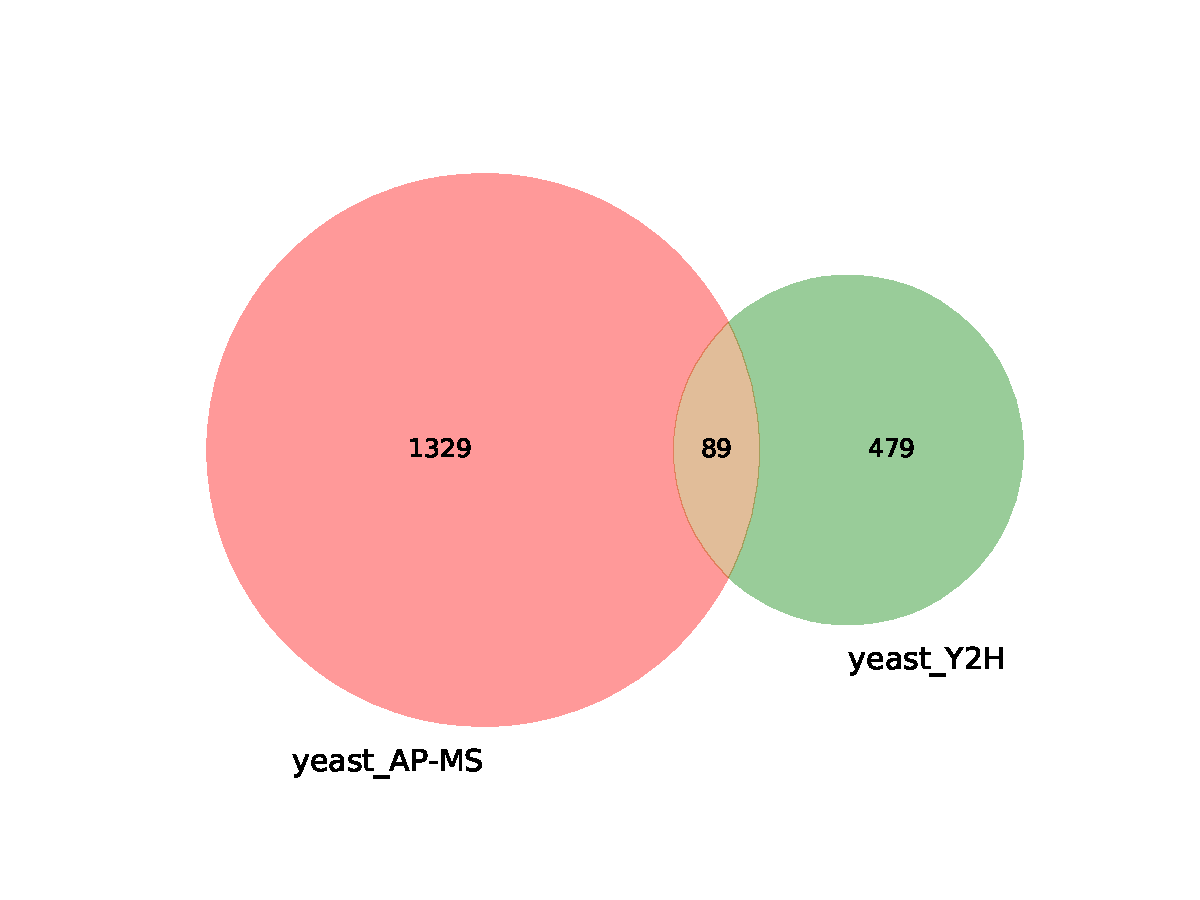
\includegraphics[width=.7\textwidth]{./schemes/venn2_coherence_yeast_AP-MS-yeast_Y2H.pdf}\\
%        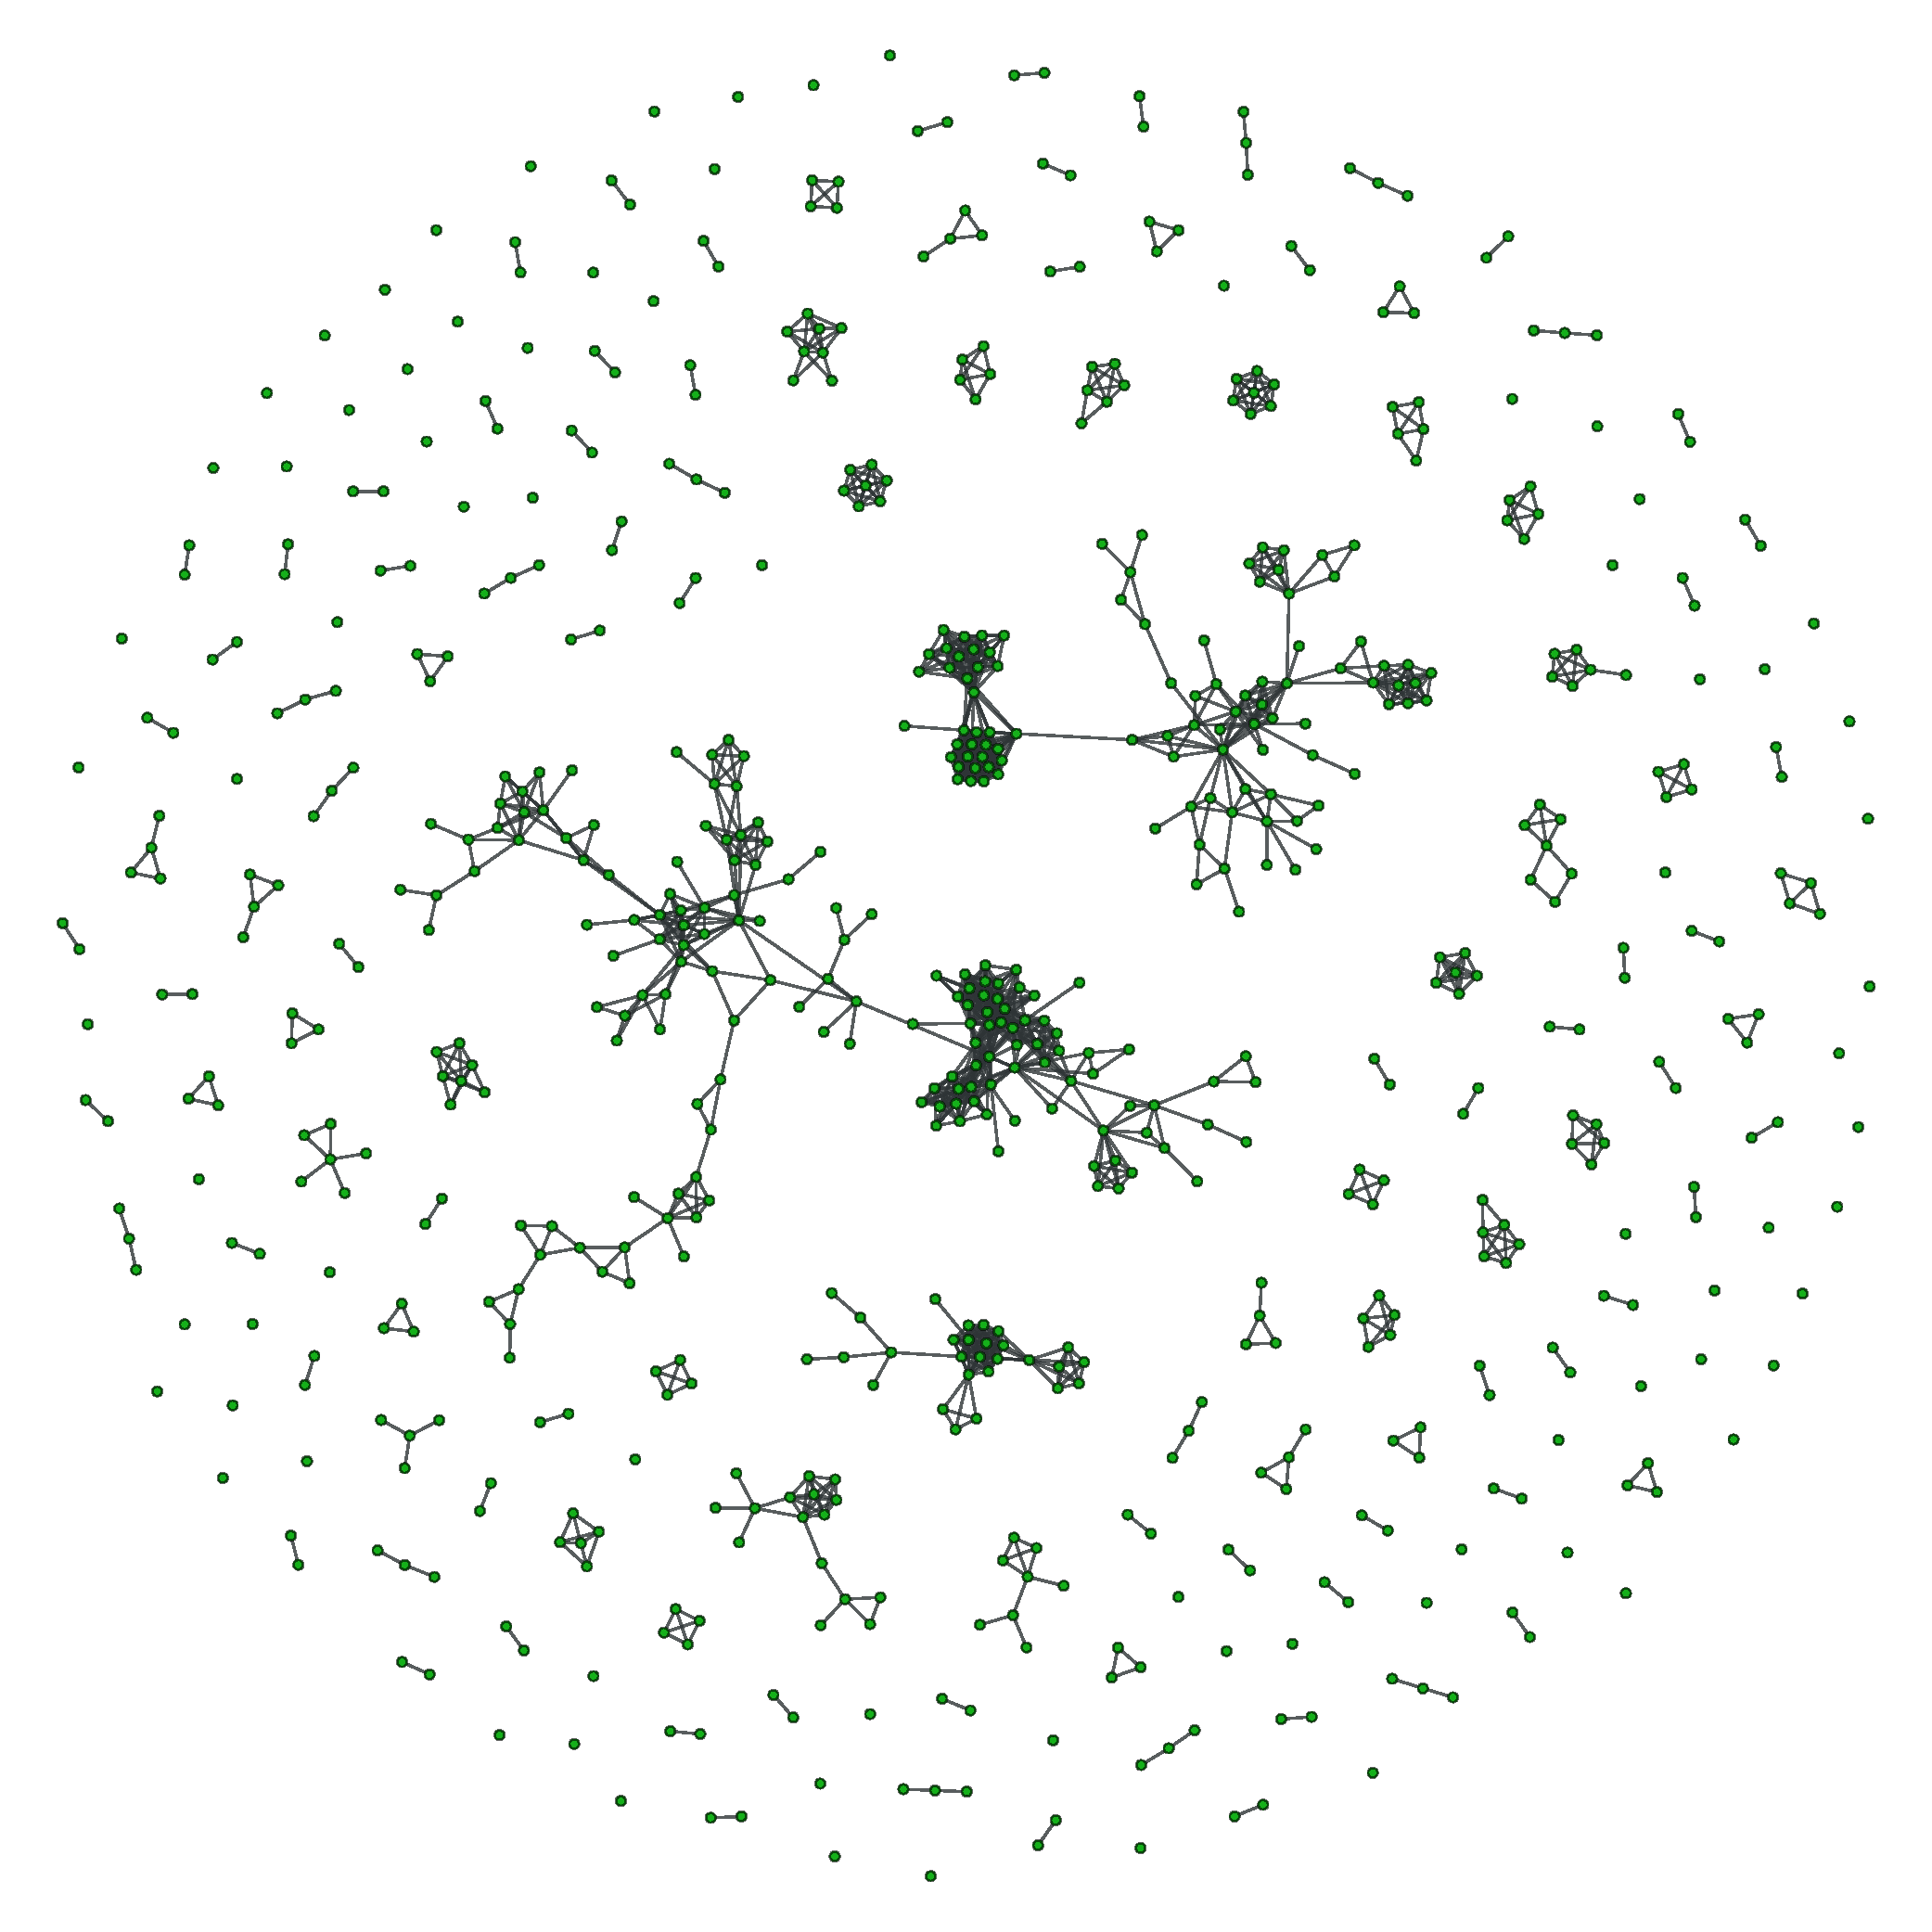
\includegraphics[width=.45\textwidth]{./schemes/subgrafo_APMS_ap_ms_y2h-gml.pdf}
%        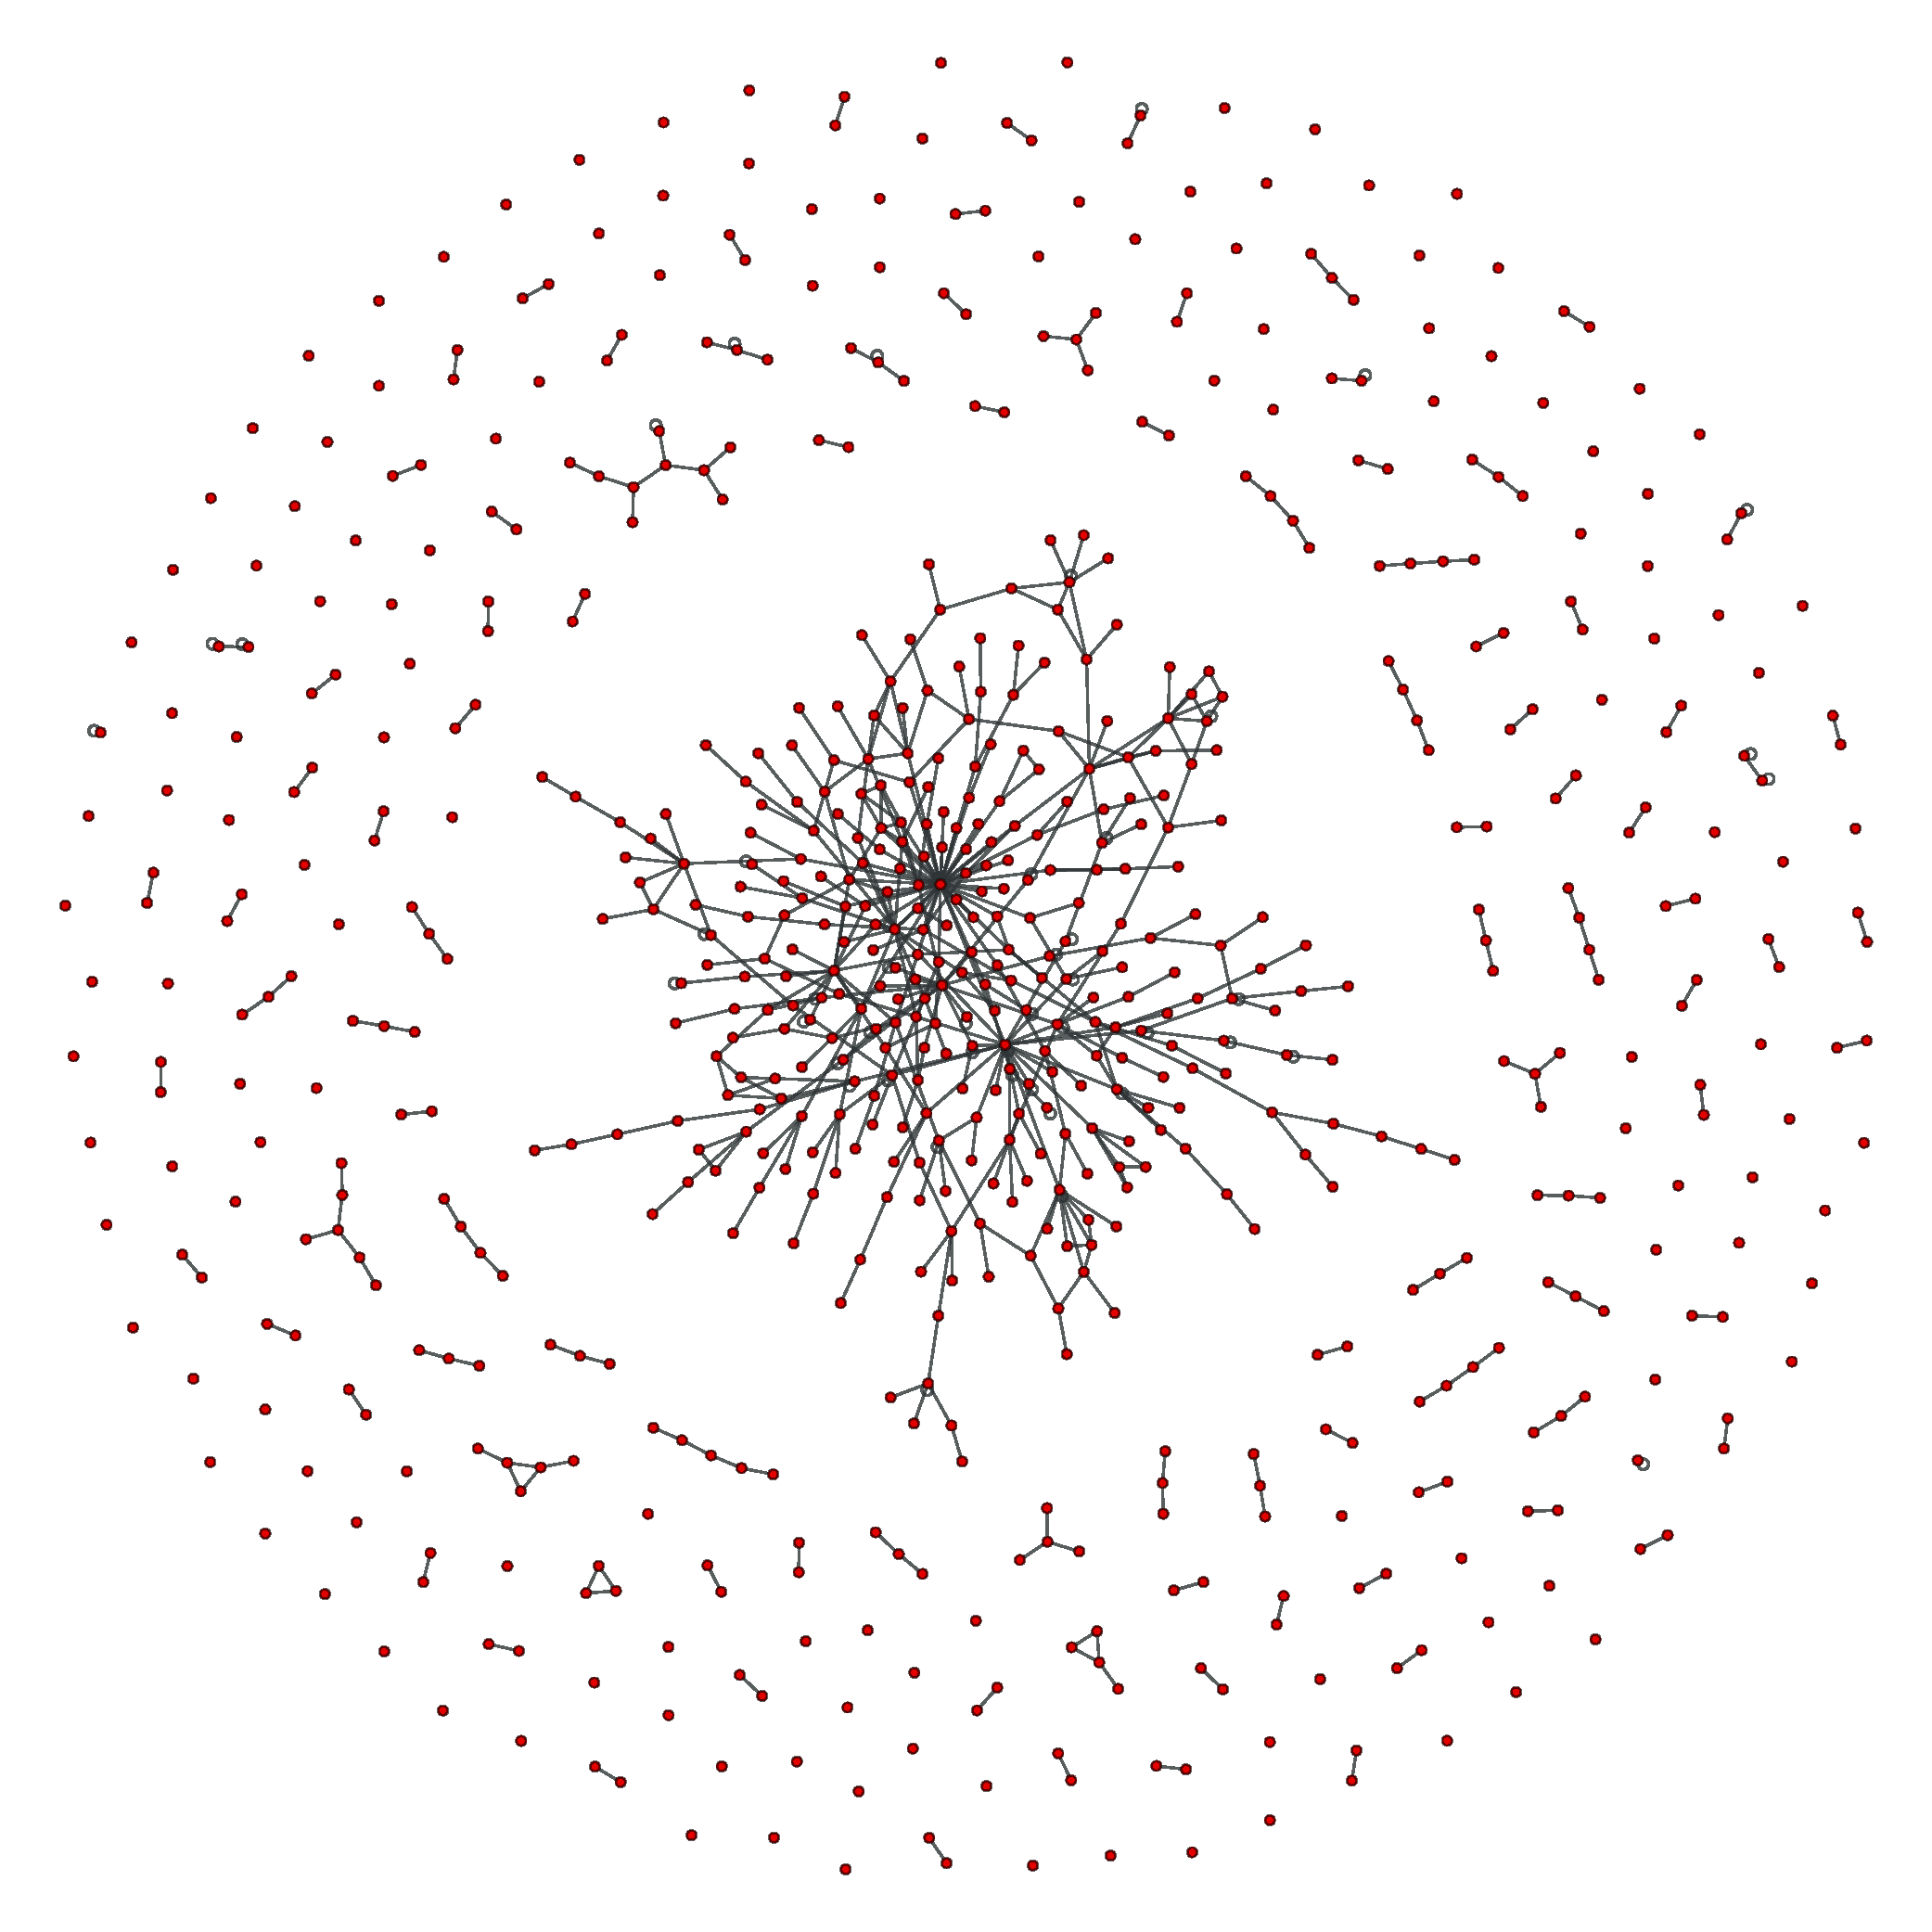
\includegraphics[width=.45\textwidth]{./schemes/subgrafo_Y2H_ap_ms_y2h-gml.pdf}
%        \caption{\label{fig:apms-y2h} AP-MS/Y2H}
%    \end{subfigure}
%    \begin{subfigure}[b]{0.3\columnwidth}
%        \centering
%        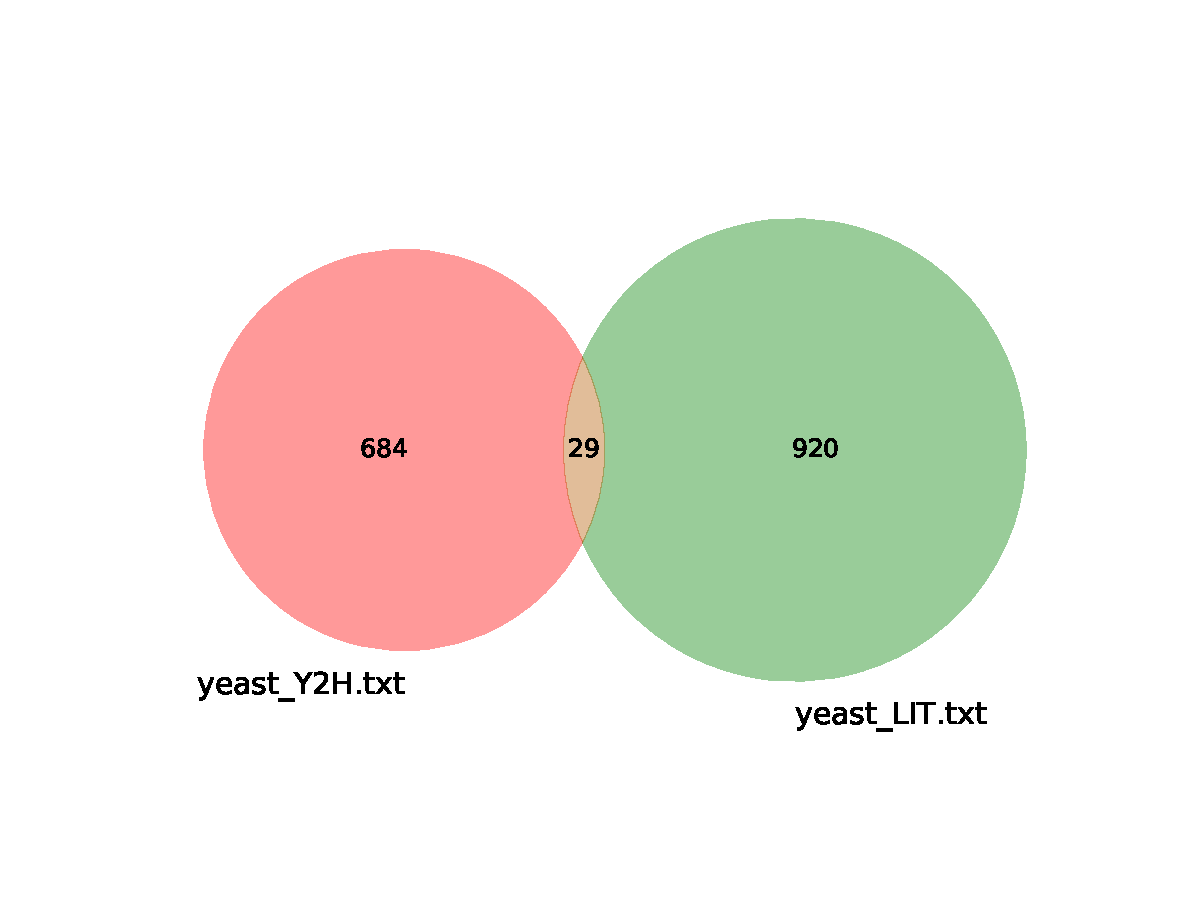
\includegraphics[width=.7\textwidth]{./schemes/venn2_coherence_yeast_Y2H-yeast_LIT.pdf}\\
%        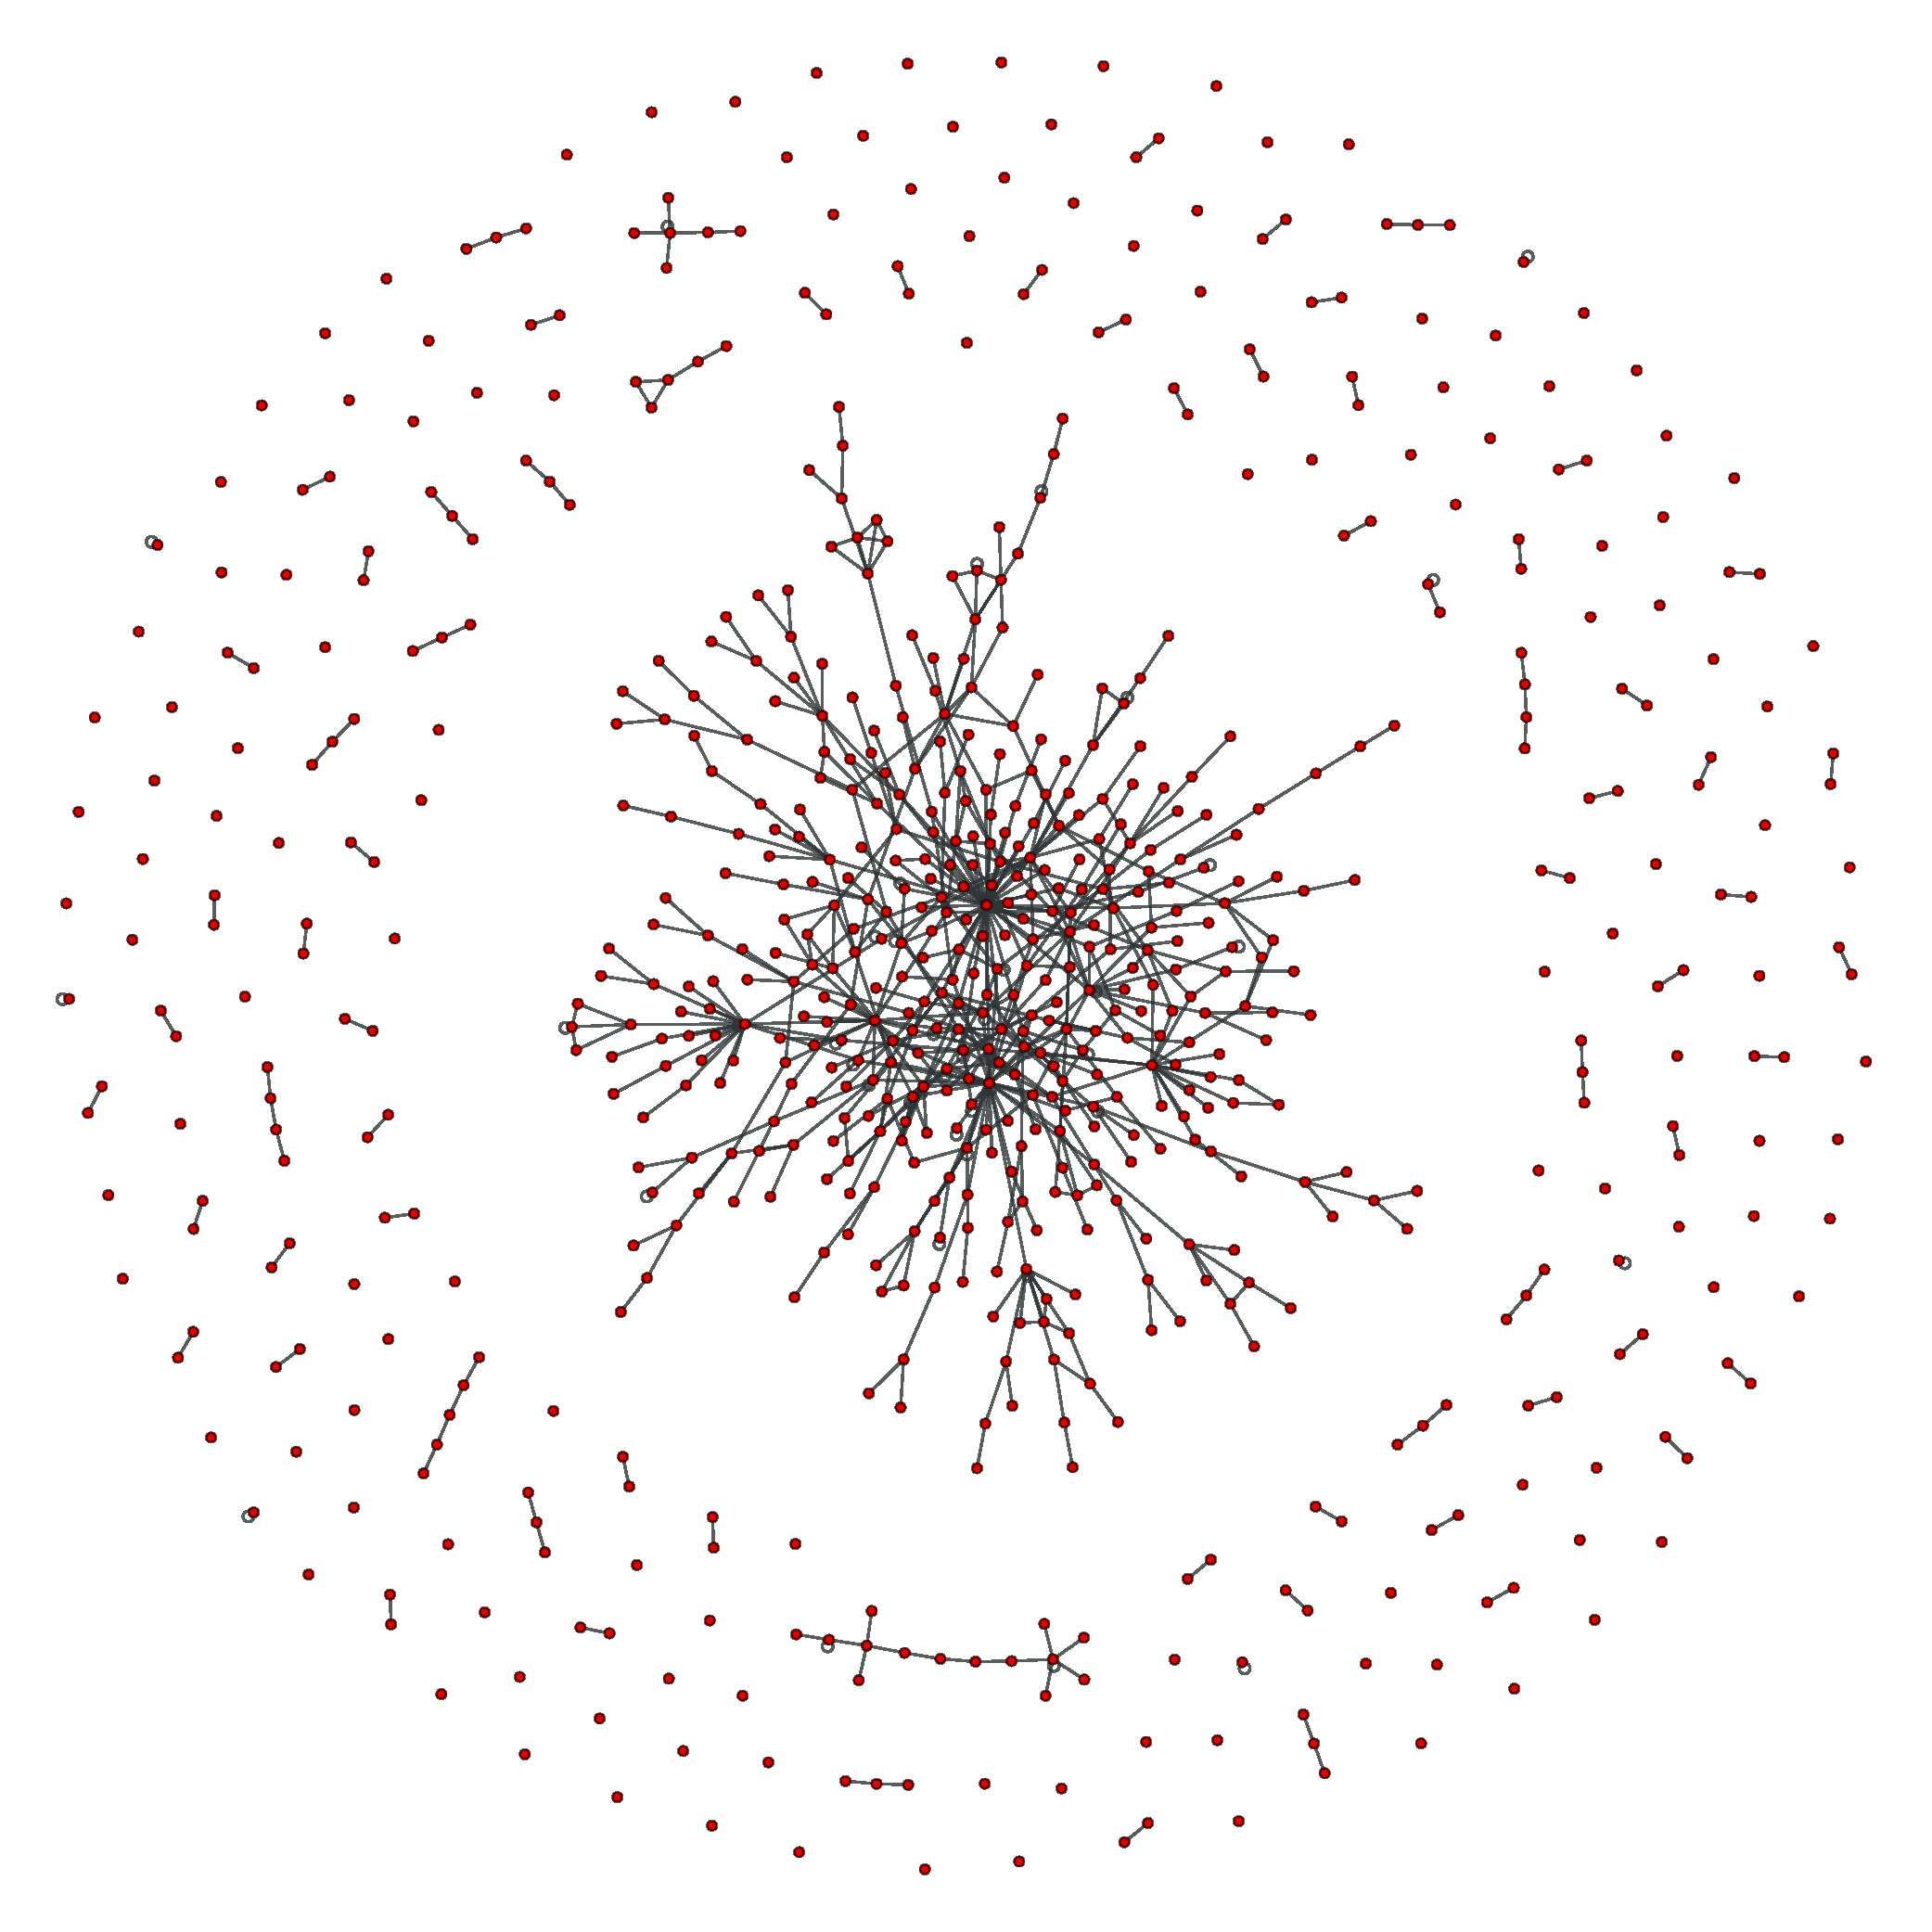
\includegraphics[width=.45\textwidth]{./schemes/subgrafo_Y2H_y2h_lit-gml.pdf}
%        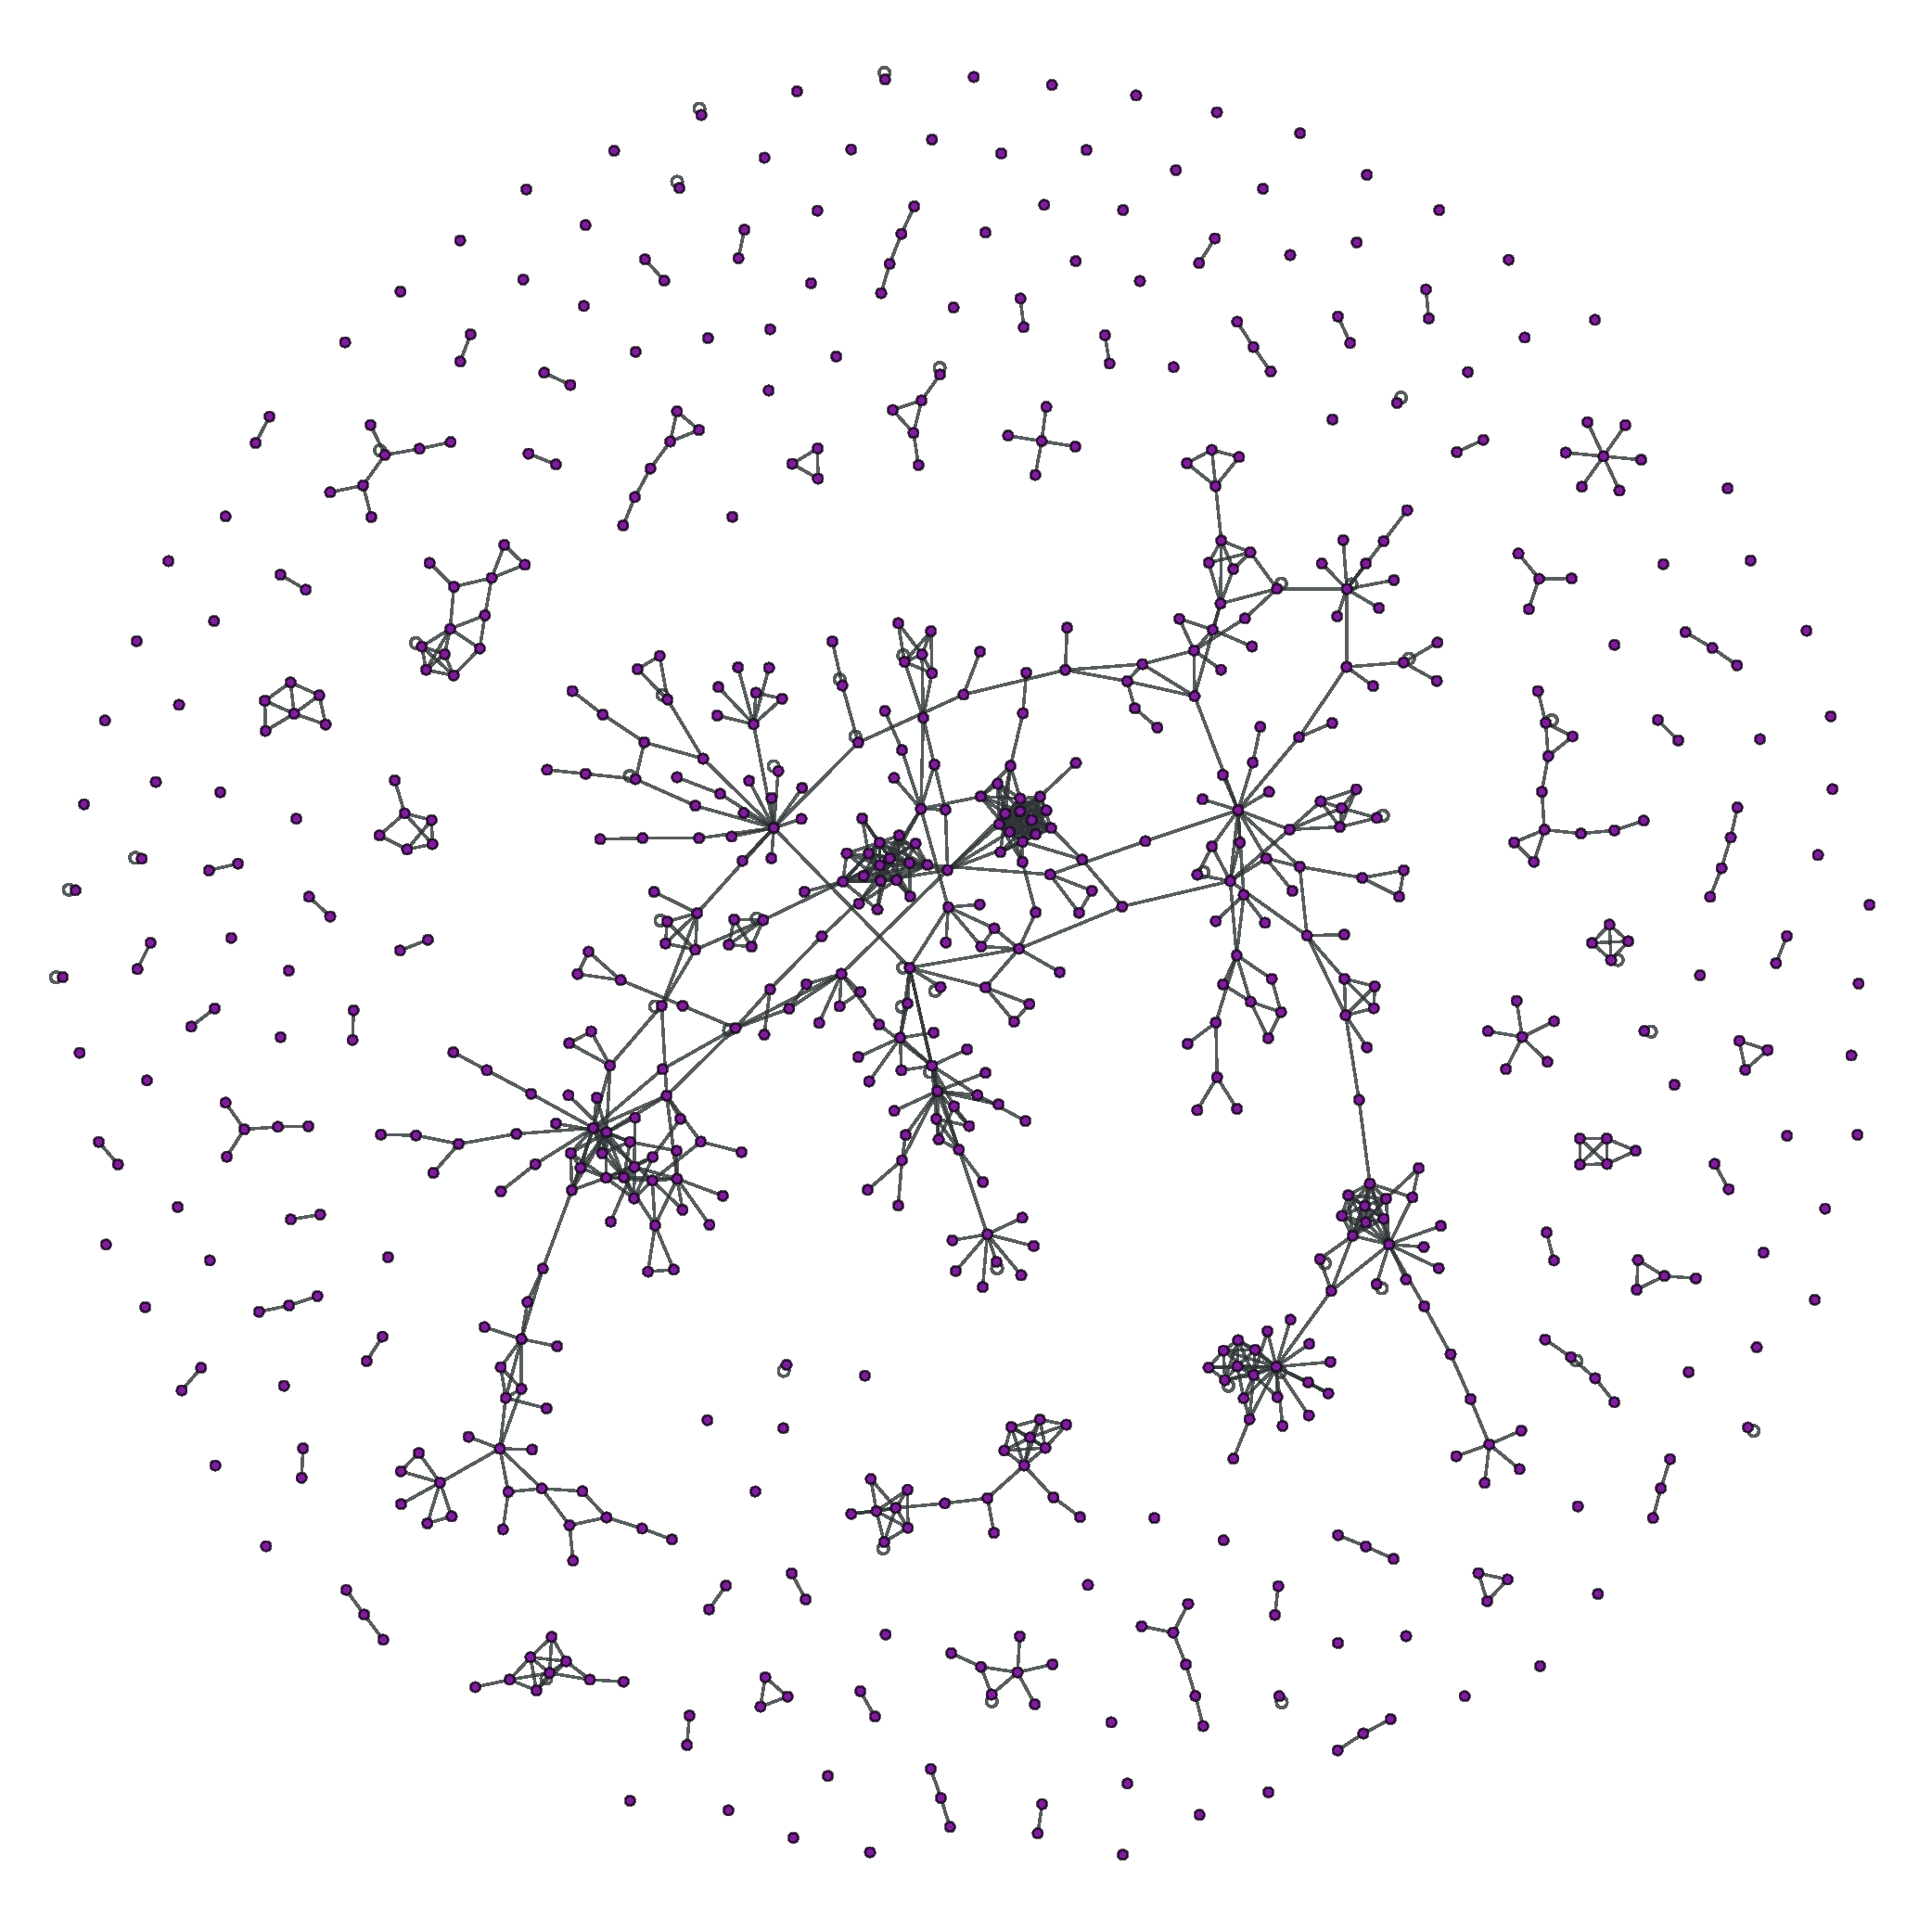
\includegraphics[width=.45\textwidth]{./schemes/subgrafo_LIT_y2h_lit-gml.pdf}
%        \caption{\label{fig:y2h-lit} Y2H/LIT}
%    \end{subfigure}
%    \caption{\label{fig:subgrafos} Coherencia entre links para cada par de redes y los respectivos subgrafos de cada red }
%\end{figure}
%
%Adicionalmente se muestran las coherencias
%a pares y los subgrafos inducidos en la figura~\ref{fig:subgrafos}. Cabe notar que, a pesar que en los subgrafos
%de la cobertura entre AP-MS y LIT podr\'ian parecer \textit{similares}, las coherencias entre links en todos los casos son
%escasas respecto a la cantidad total de links en cada subgrafo.


    \newpage
    
\section{Impacto de remoción.}

\par En esta sección estudiamos el impacto de remover proteínas que son centrales bajo diferentes criterios y lo comparamos con el impacto de remover las proteíans catalogadas como esenciales. Según \cite{jeong2000}, un nodo con alto grado en la red de interacciones tiene más probabilidad de ser esencial que la esperada por azar, debido a que actúa de intermediario entre nodos de menor grado. Sin embargo, cabe la posibilidad de que no sea el número de vecinos inmediatos lo que determina la importancia de una proteína, sino algún otra propiedad topológica más global.
\par En las figura \ref{fig:remocion} estudiamos cómo se modifica el tamaño relativo (al tamaño de la componente de la red original) de la componente más grande al remover los nodos catalogados como centrales según diferentes criterios, para las cuatro redes estudiadas. Comparamos estos resultados con el caso de remover las proteínas esenciales, y con remover nodos al azar sin más criterio. Los criterios utilizados fueron: grado del nodo, centralidad de betweenness, centralidad de Bonacich, y subgraph centrality. 
\par De la figura \ref{fig:remocion} concluímos que el impacto de remoción de nodos centrales es mayor que la remoción de los nodos esenciales, que en algunos casos es equivalente a remover nodos al azar. Esto daría la noción que la esencialidad de una proteína no está ligada a su rol en la red de interacciones.
\par Cabe destacar que el proceso de remoción consistió en calcular la centralidad de cada nodo en la red original, y removerlos de mayor a menor sin volver a realizar el cálculo. Esto implica que removimos los nodos que son centrales en la red original. Si se decide remover el nodo con mayor centralidad luego de realizar una remoción, el impacto de la misma es mayor que el criterio que utilizamos, sin embargo le daríamos el rol de central a un nodo que quizás no cumple en la red original. A modo de criterio alternativo, incluímos un gráfico análogo a \ref{fig:remocion} en la figura \ref{fig:remocion_alternativo}, donde se puede observar que el impacto de remoción es mayor.
 
\begin{figure}
\centering
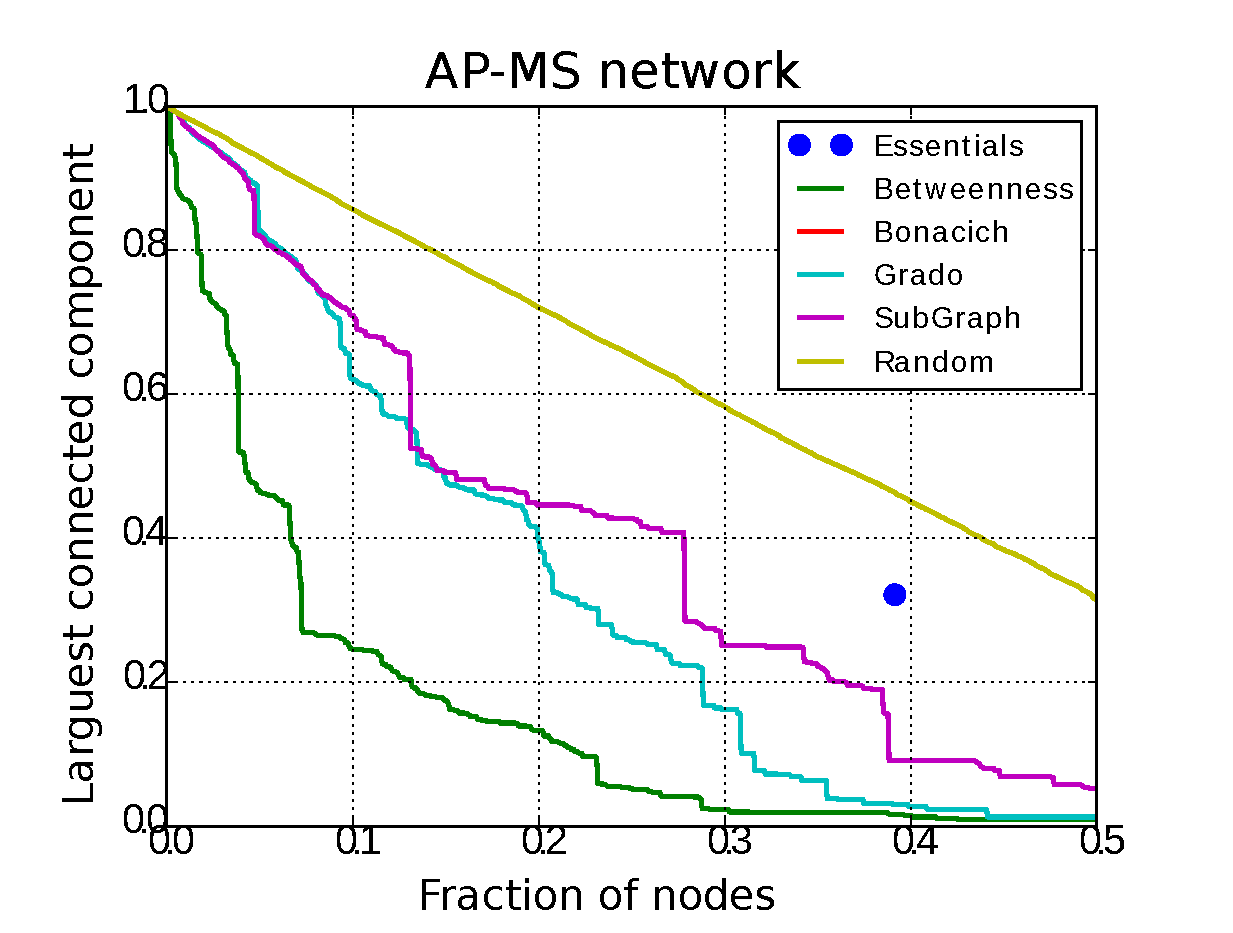
\includegraphics[scale = 0.30]{figuras/AP-MS_b} 
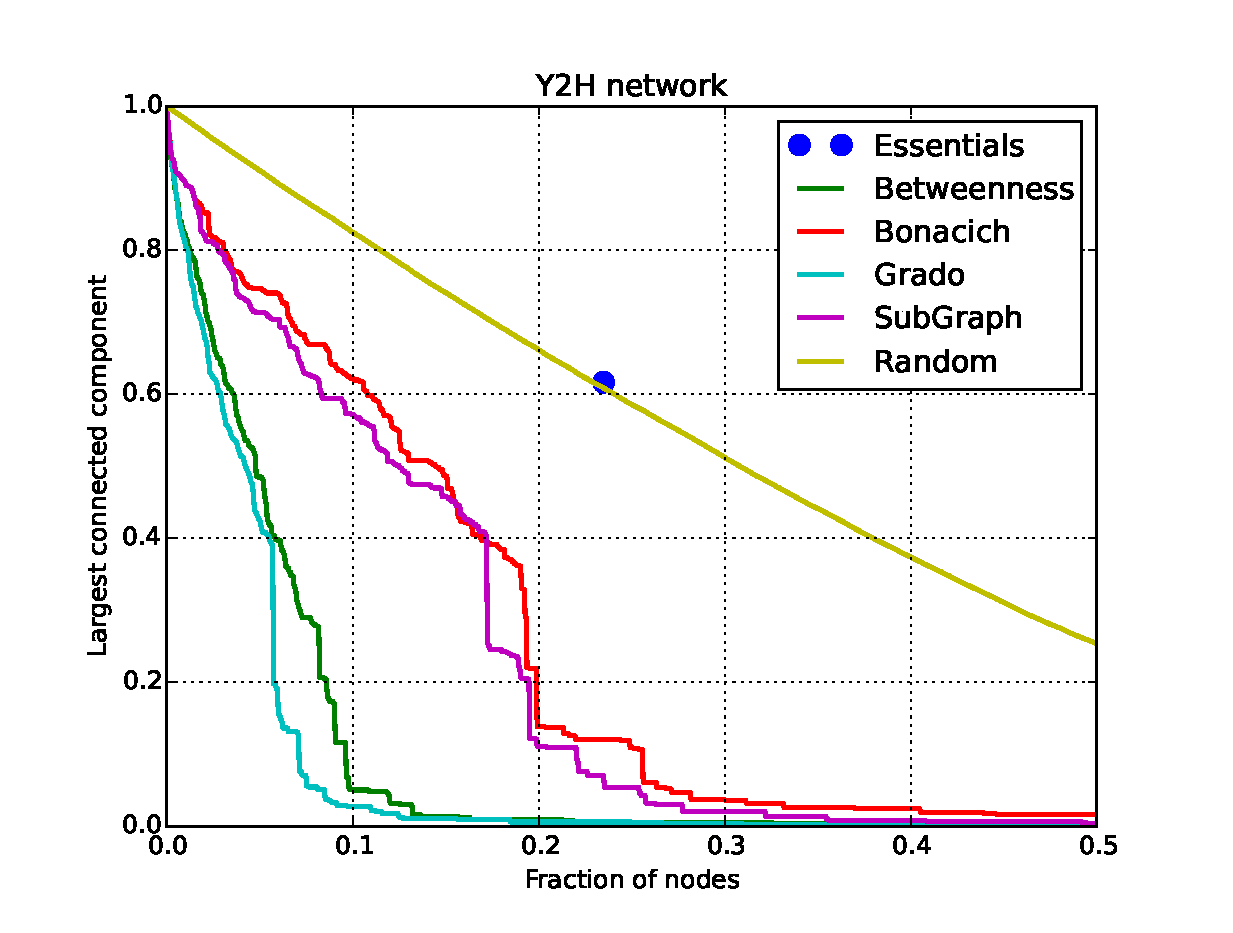
\includegraphics[scale = 0.30]{figuras/Y2H_b} \\
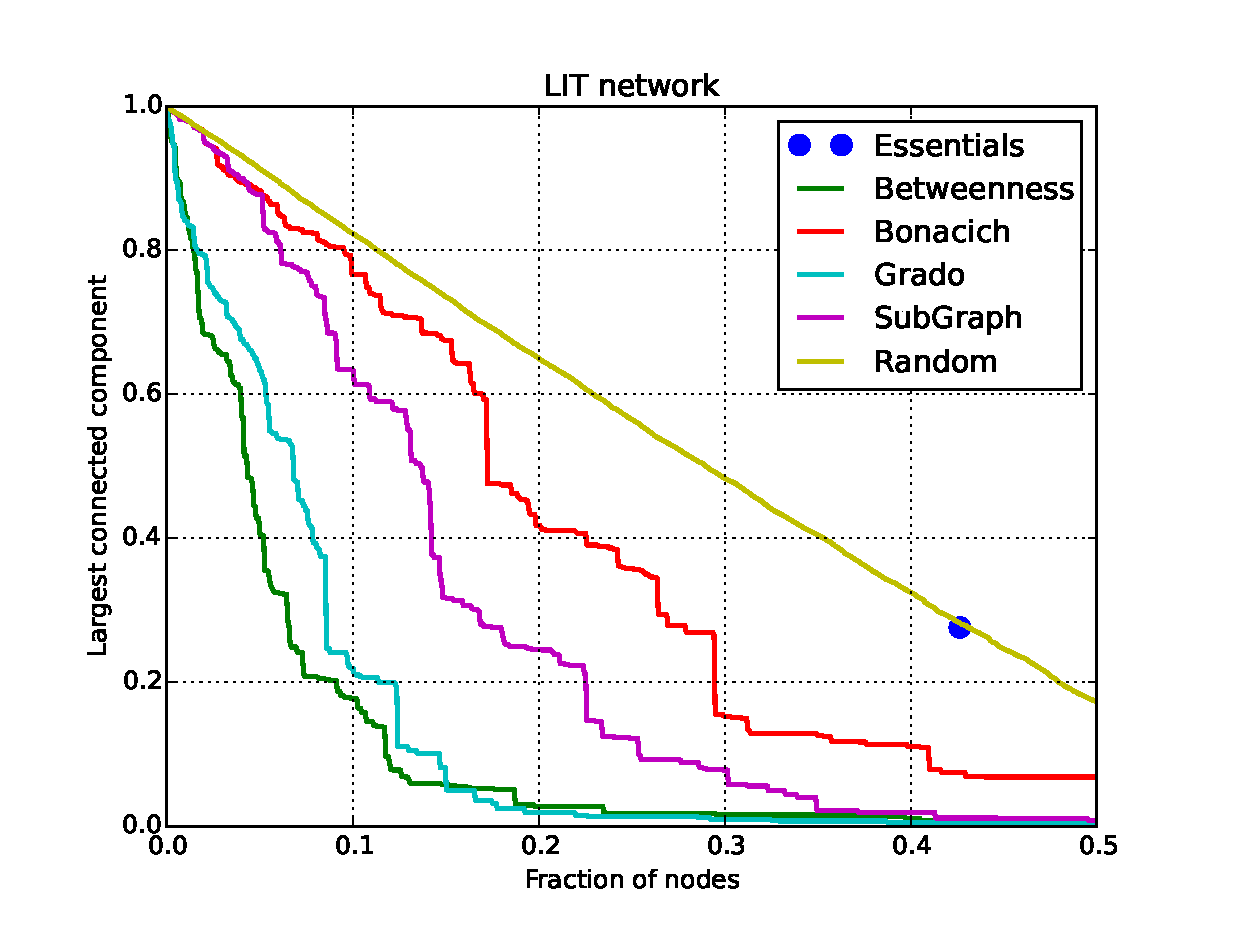
\includegraphics[scale = 0.30]{figuras/LIT_b} 
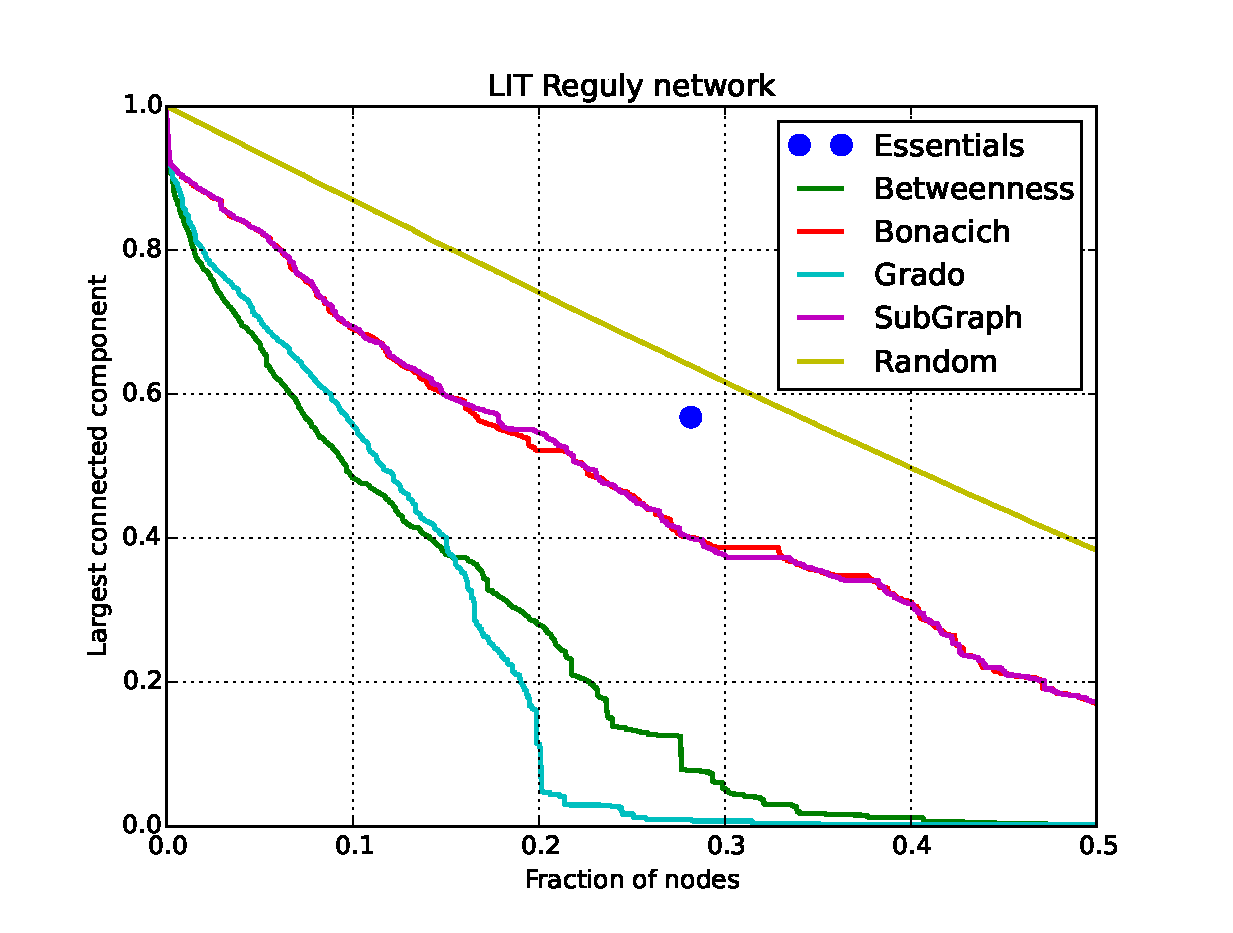
\includegraphics[scale = 0.30]{figuras/LIT_Reguly_b} 
\caption{Tamaño relativo de la componente conectada más grande a medida que se remueven los nodos ordenados con diferentes criterios de centralidad. Se incluye el impacto de remover las proteínas esenciales y remover nodos al azar. En todos los casos se puede observar que el impacto de remoción (caída del tamaño del fragmento conectado) es mucho más alto al utilizar un criterio de centralidad en comparación con la remoción de las esenciales, que en algunos casos, prácticamente coincide con la remoción al azar.}
\label{fig:remocion}
\end{figure}

\begin{figure}
\centering
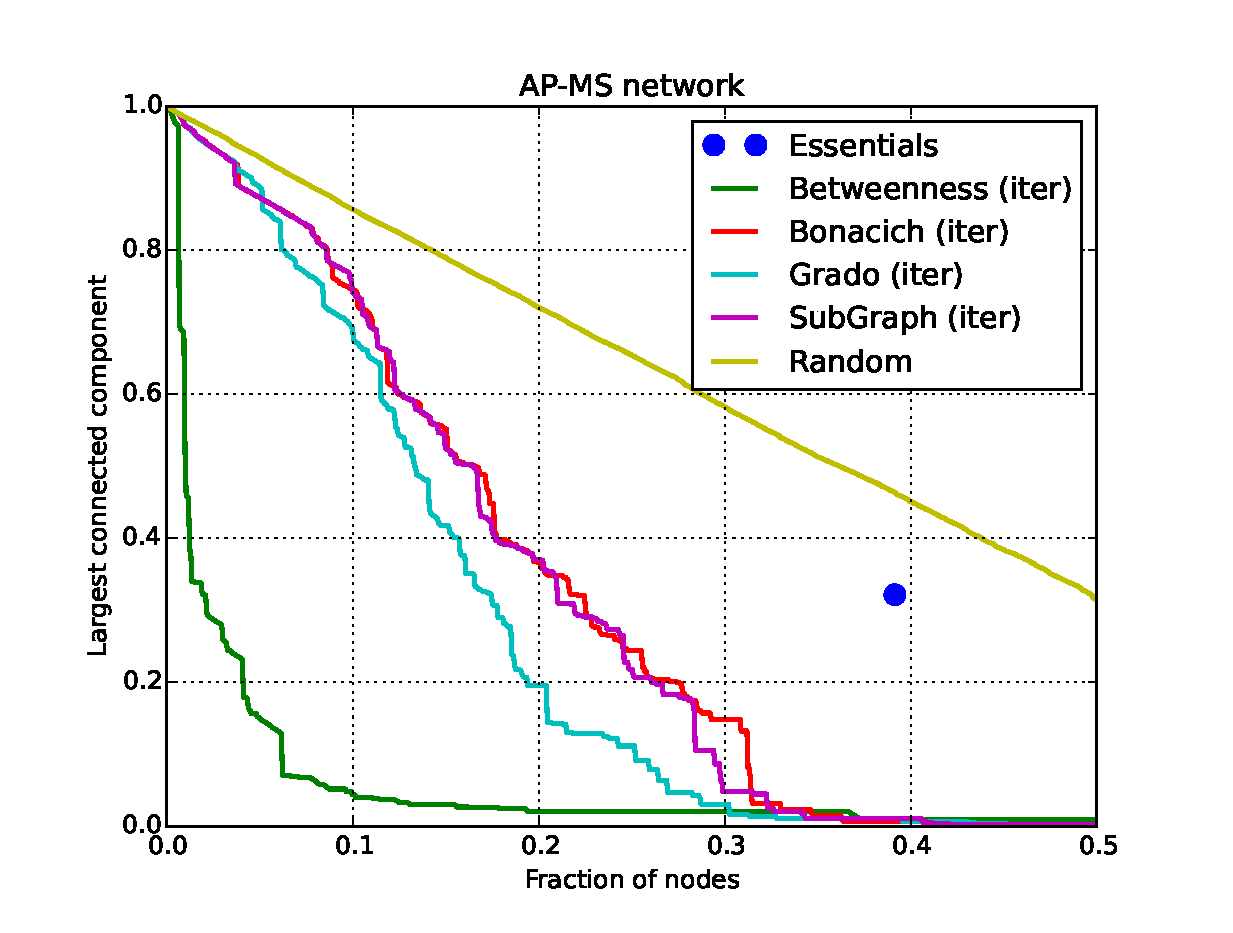
\includegraphics[scale = 0.30]{figuras/AP-MS} 
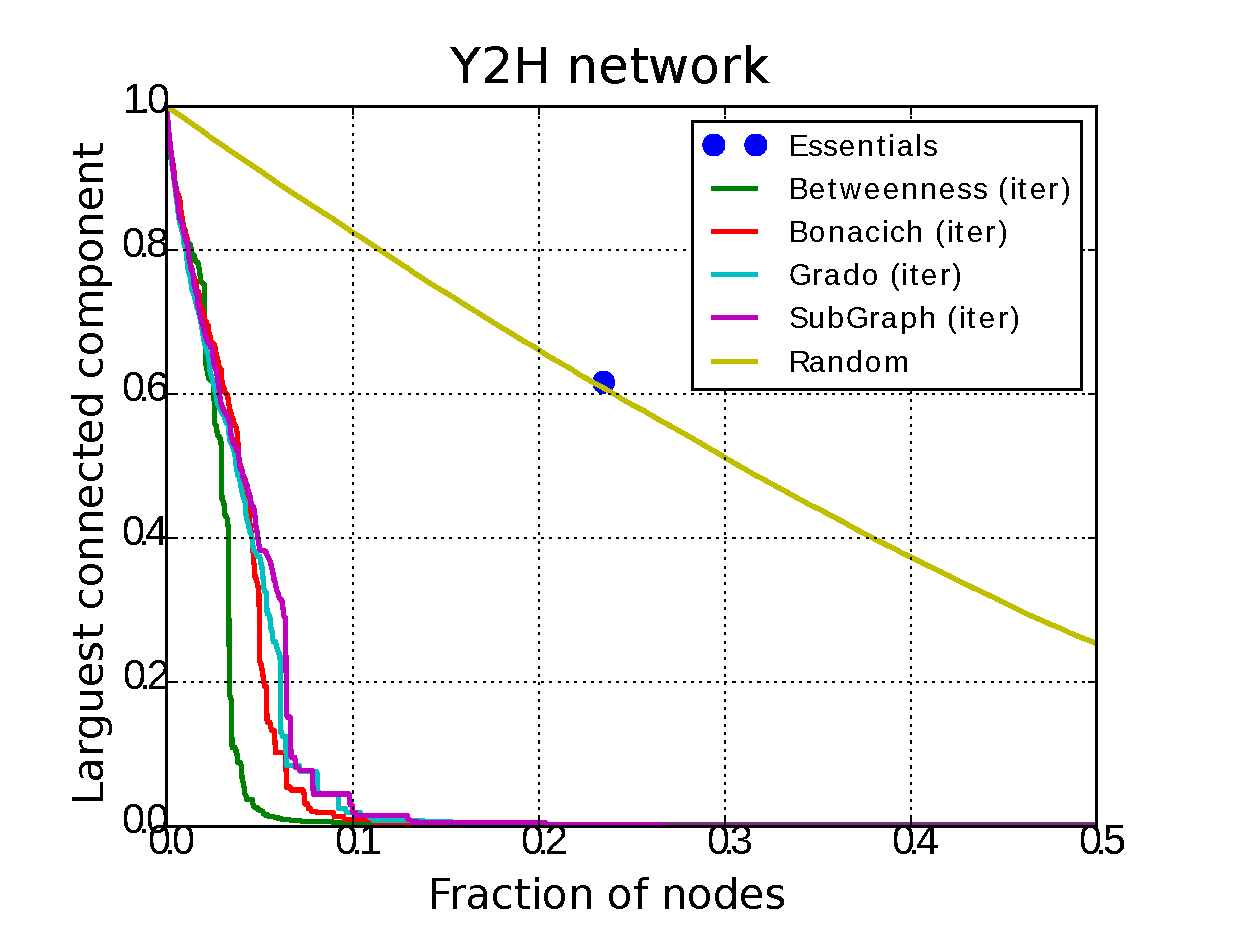
\includegraphics[scale = 0.30]{figuras/Y2H} \\
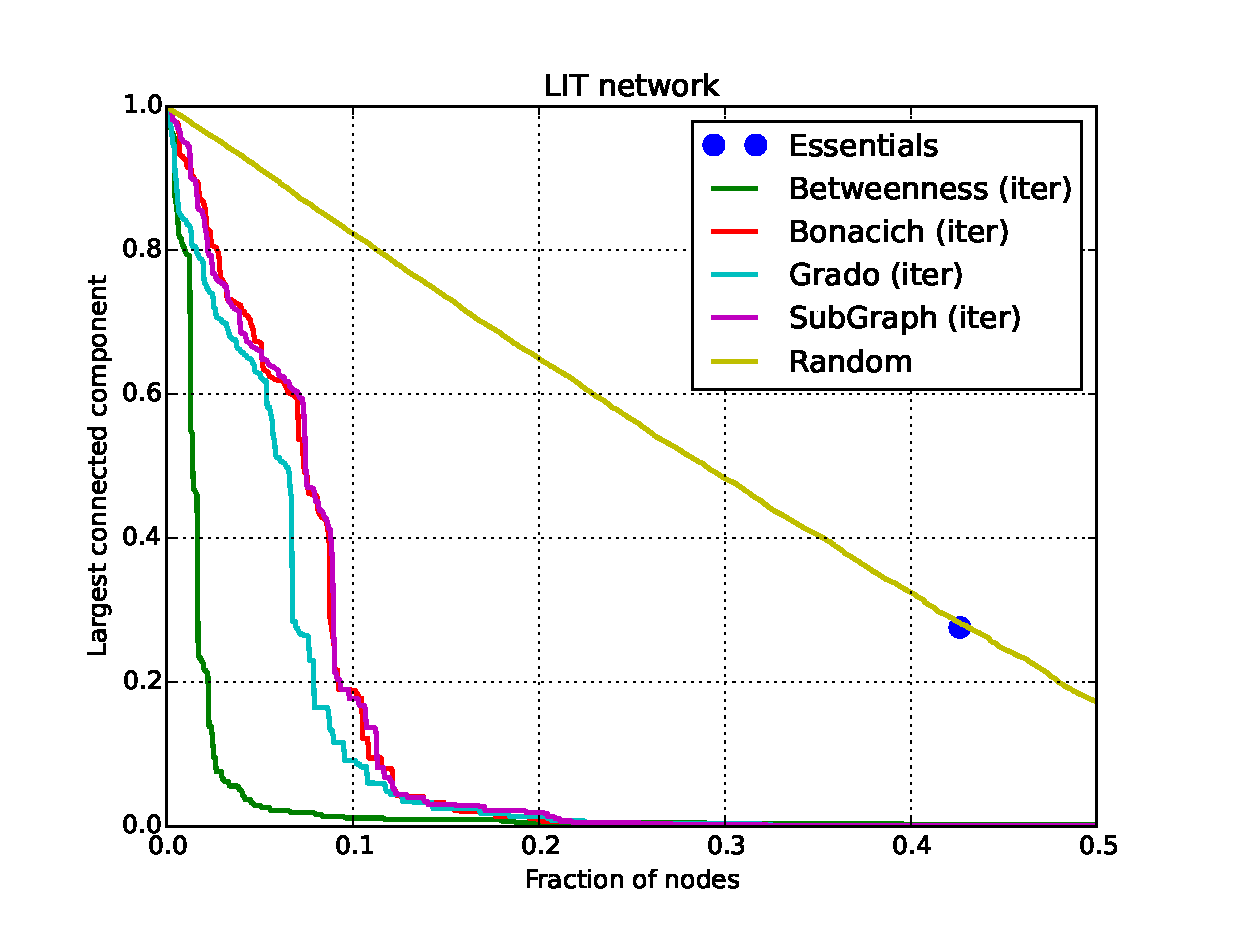
\includegraphics[scale = 0.30]{figuras/LIT} 
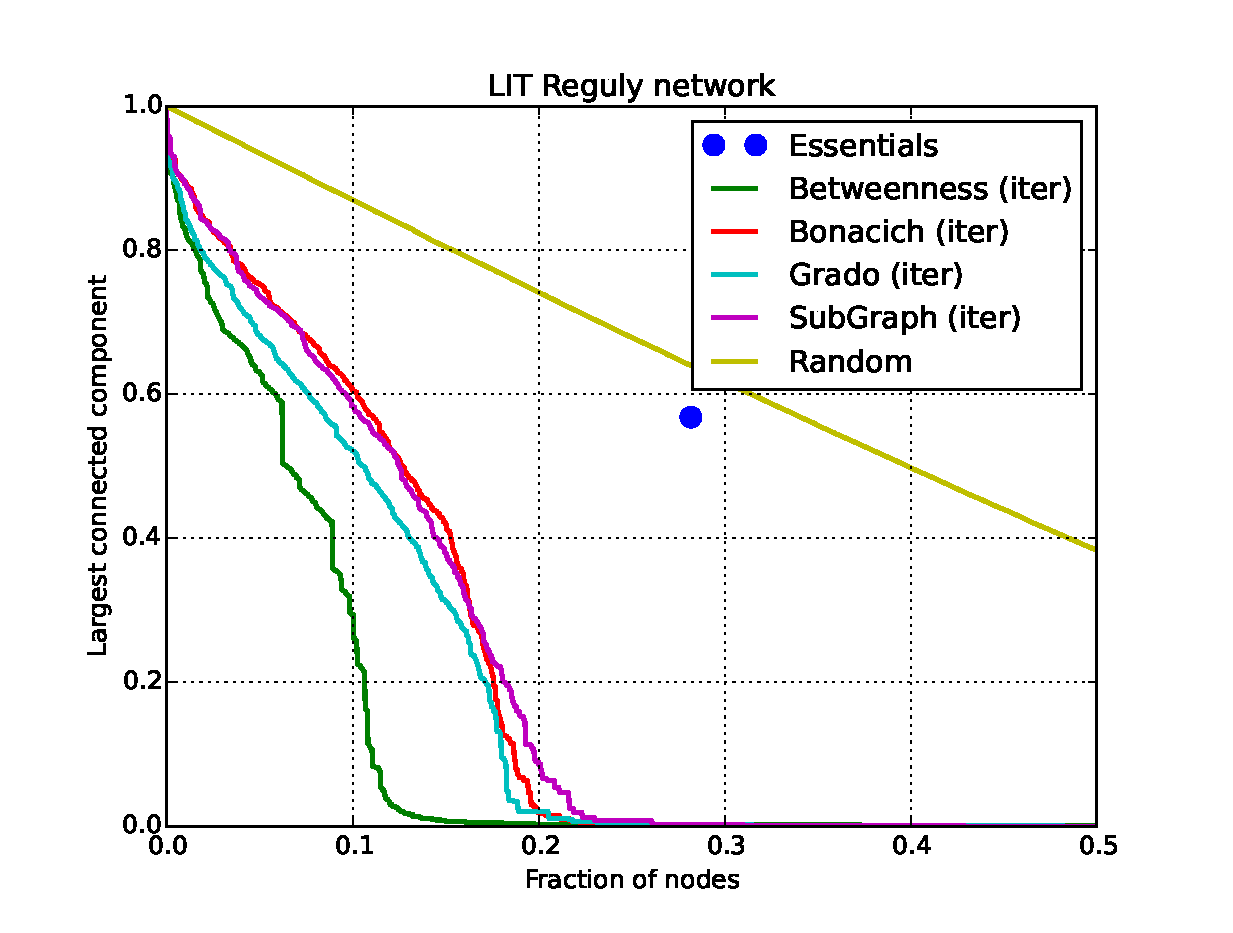
\includegraphics[scale = 0.30]{figuras/LIT_Reguly} 
\caption{Tamaño relativo de la componente conectada más grande a medida que se remueven los nodos ordenados con diferentes criterios de centralidad, en forma iterativa, es decir, se remueve el nodo más central en la configuración actual de la red. Se puede observar que el impacto de remoción es mayor que el de la figure \ref{fig:remocion}.}
\label{fig:remocion_alternativo}
\end{figure}

\subsection{Remoción de nodos al azar.}

\par En las figuras \ref{fig:remocion} y \ref{fig:remocion_alternativo}, la remción de nodos al azar no siguió ningún criterio particular. En esta sección estudiaremos el impacto de tomar nodos al azar no esenciales, pero cuya distribución de grado sea equivalente a la de los nodos esenciales presentes en la red. Tomaremos nuevamente el tamaño relativo de la componente más grande como impacto de remoción. Cabe recordar que un tamaño relativo menor implica un impacto de remoción mayor.
\par En la tabla \ref{table:remocion}, comparamos el impacto de remover los nodos esenciales con la remoción de nodos no esenciales, con distribución de grado equivalente. El criterio tomado consistió en, dado un nodo esencial, tomar uno no esencial con el grado más cercano posible.
\begin{table}
\centering
\begin{tabular}{c c c c}
\hline \hline
Red & Tr(Esenc.) & Tr(No Esenc.) & Nodos removidos \\
\hline
AP-MS & 0.32 & $0.38 \pm 0.02$ & 615 \\
LIT & 0.276 & $0.417 \pm 0.003$ & 636 \\
Y2H & 0.62 & $0.61 \pm 0.01$ & 459 \\
LIT-Reguly & 0.568 & $0.536 \pm 0.005$ & 903 \\
\hline
\end{tabular}
\caption{Tamaño relativo de la componente conectada más grande. Salvo en la red LIT, donde la remoción de nodos esenciales marca da una caída del tamaño más abrupta que la remoción al azar, en los otros casos, el impacto es equivalente.}
\label{table:remocion}
\end{table}
\par De la tabla podemos concluir que salvo en la red LIT, el impacto de remoción es prácticamente el mismo que remover nodos no esenciales con la misma distribución de grado. Con lo cual la hipótesis de que la esencialidad de un nodo se debe a su grado queda descartada.


    

    %\input{jeong}

    %\section{Hip\'otesis de interacciones esenciales~\citep{he2006}}
Como hemos mostrado en la secci\'on \ref{sec:jeong} la correlaci\'on vista por Jeong es corroborada, sin embargo su hip\'otesis
de esencialidad debido centralidad por grado no responde al comportamiento real de las redes. He y sus colegas plantean una
hip\'otesis alternativa: La esencialidad se debe a la participaci\'on en interacciones esenciales y no esencialidad 
\textit{unitaria} como pensaba Jeong. Bajo esta hip\'otesis la regla de Centralidad-Letalidad se explica debido a que 
los hubs, al tener mayor cantidad de interacciones, tienen mayor probabilidad de pertenecer a una interacci\'on esencial.

El modelo de He considera dos condiciones de esencialidad: La prote\'ina participa en una interacci\'on esencial representada
en la red con una probabilidad $\alpha$ \'o la prote\'ina es esencial debido a alg\'un otro factor que la red no es capaz de
mostrar. As\'i la probabilidad de que un nodo de grado $k$ no participe en una interacc\'ion esencial es 
$(1-\alpha)(1-\alpha)\cdots(1-\alpha) = (1-\alpha)^k$ y la probabilidad de no ser esencial debido a otra raz\'on es $(1-\beta)$.
Luego, la probabilidad de no ser esencial es

\begin{align}
    \label{eq:ne}
    1-P_E(k) &= (1-\beta)(1-\alpha)^k\\
    \intertext{finalmente, la probabilidad de esencialidad es}
    P_E(k) &= 1 - (1-\beta)(1-\alpha)^k
\end{align}


A continuaci\'on evaluaremos la calidad de esta hip\'otesis a trav\'es de estimaciones de las probabilidades por dos m\'etodos 
descritos en el trabajo de He y colegas. Cabe se\~nalar que, para lo que resta del an\'alisis, la red AP-MS no ser\'a considerada,
debido a que \citet{he2006} hace referencia redes construidas a partir de asociaci\'on de complejos proteicos podr\'ian 
presentar comportamientos an\'omalos.

\subsection{M\'etodo de Ajuste}
Tomando el logaritmo a la ec. \ref{eq:ne} se tiene 
\begin{align}
    \ln(1-P_E(k)) &= k \ln(1-\alpha) + \ln(1-\beta)
\end{align}
es decir, una relaci\'on lineal entre el grado y la probabilidad de no-esencialidad. \citet{he2006} mensiona que, debido a que
a mayor grado $k$ es m\'as dificil encontrar nodos con grado $k$, por lo que para sus an\'alisis utiliza un umbral superior de
$k=10$. En este trabajo se ha considerado lo mismo. La figura \ref{fig:fit} muestra los resultados del ajuste lineal para 
nuestras redes. Debido al comportamineto irregular de la red Y2H (ver figura \ref{fig:y2h}) esta fue excluida del an\'alisis.

\begin{figure}[!ht]
    \centering
    \begin{subfigure}[b]{0.4\columnwidth}
        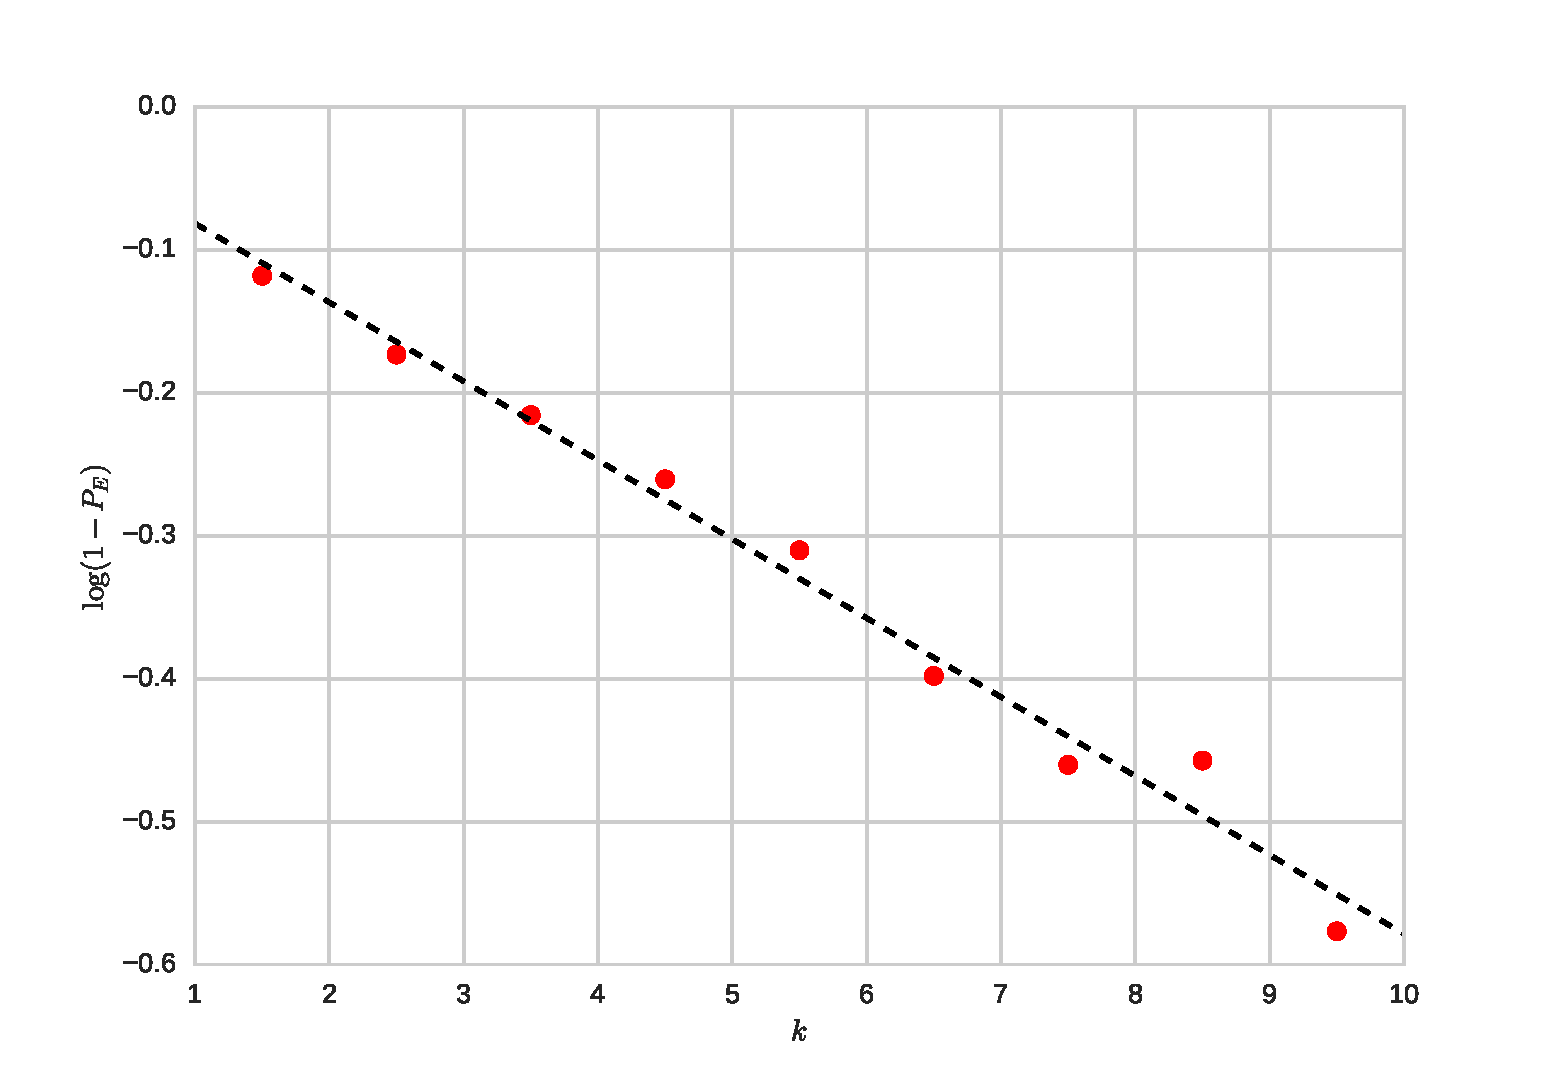
\includegraphics[width=\textwidth]{./schemes/yeast_LIT_Reguly.pdf}
        \caption{\label{fig:LITR}LIT\_Reguly}
    \end{subfigure}
    \begin{subfigure}[b]{0.4\columnwidth}
        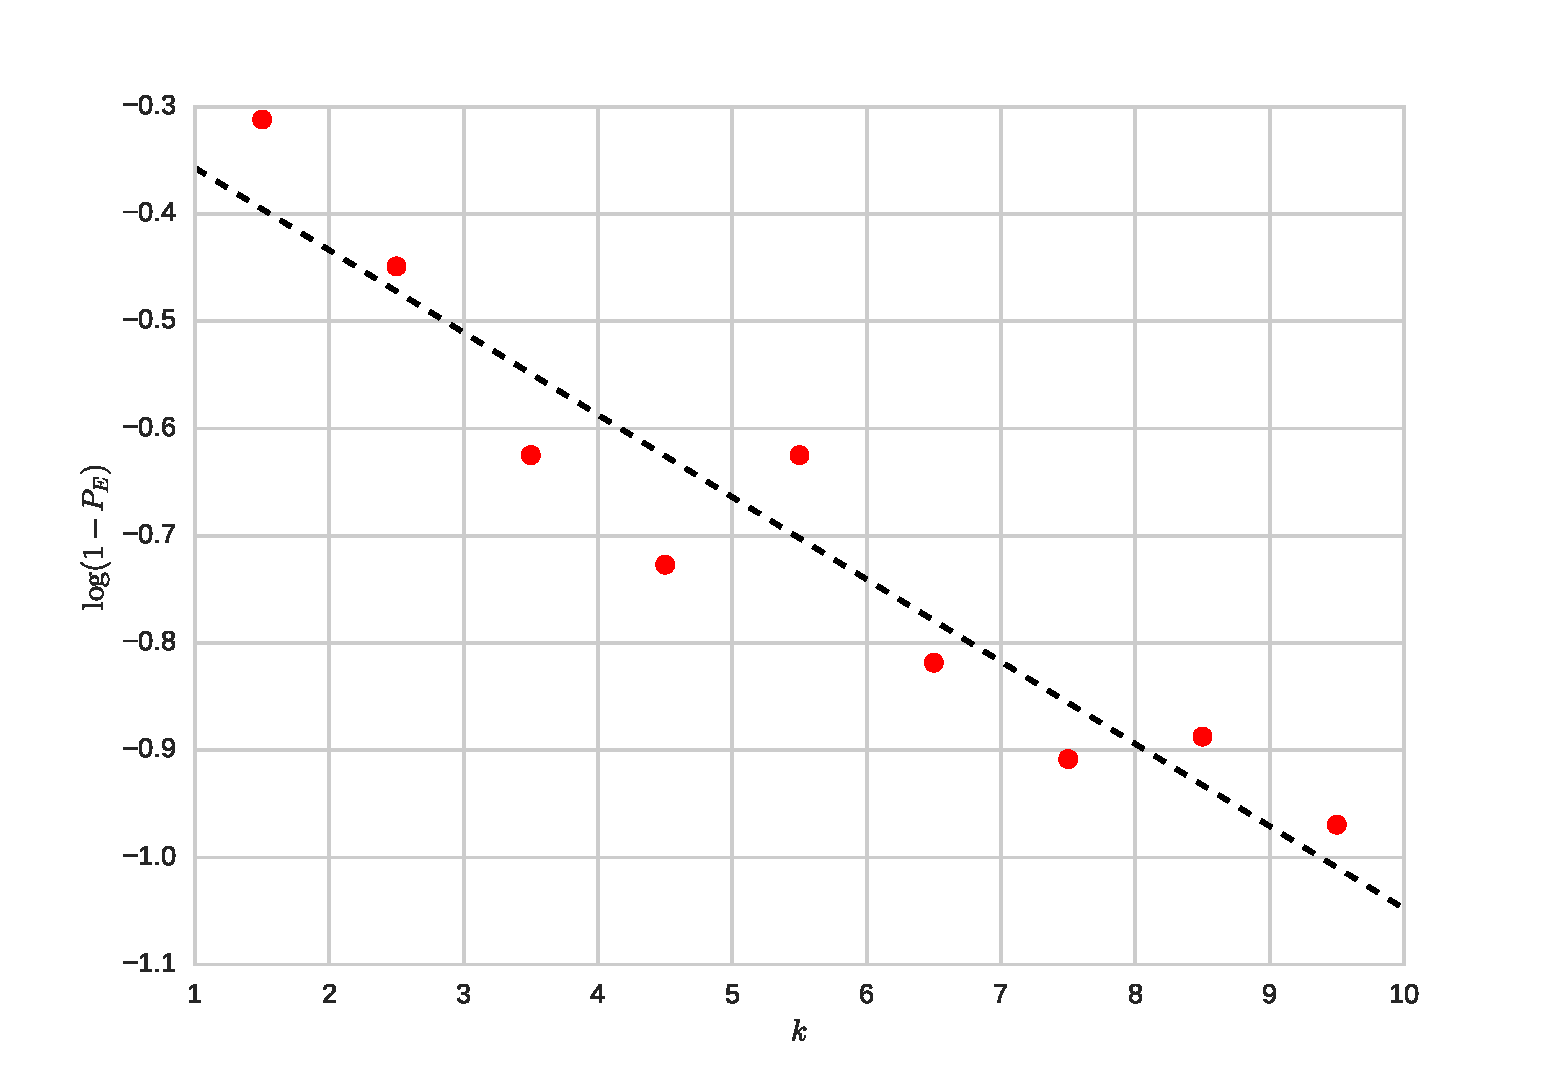
\includegraphics[width=\textwidth]{./schemes/yeast_LIT.pdf}
        \caption{\label{fig:LIT} LIT}
    \end{subfigure}
    \\
    \begin{subfigure}[b]{0.4\columnwidth}
        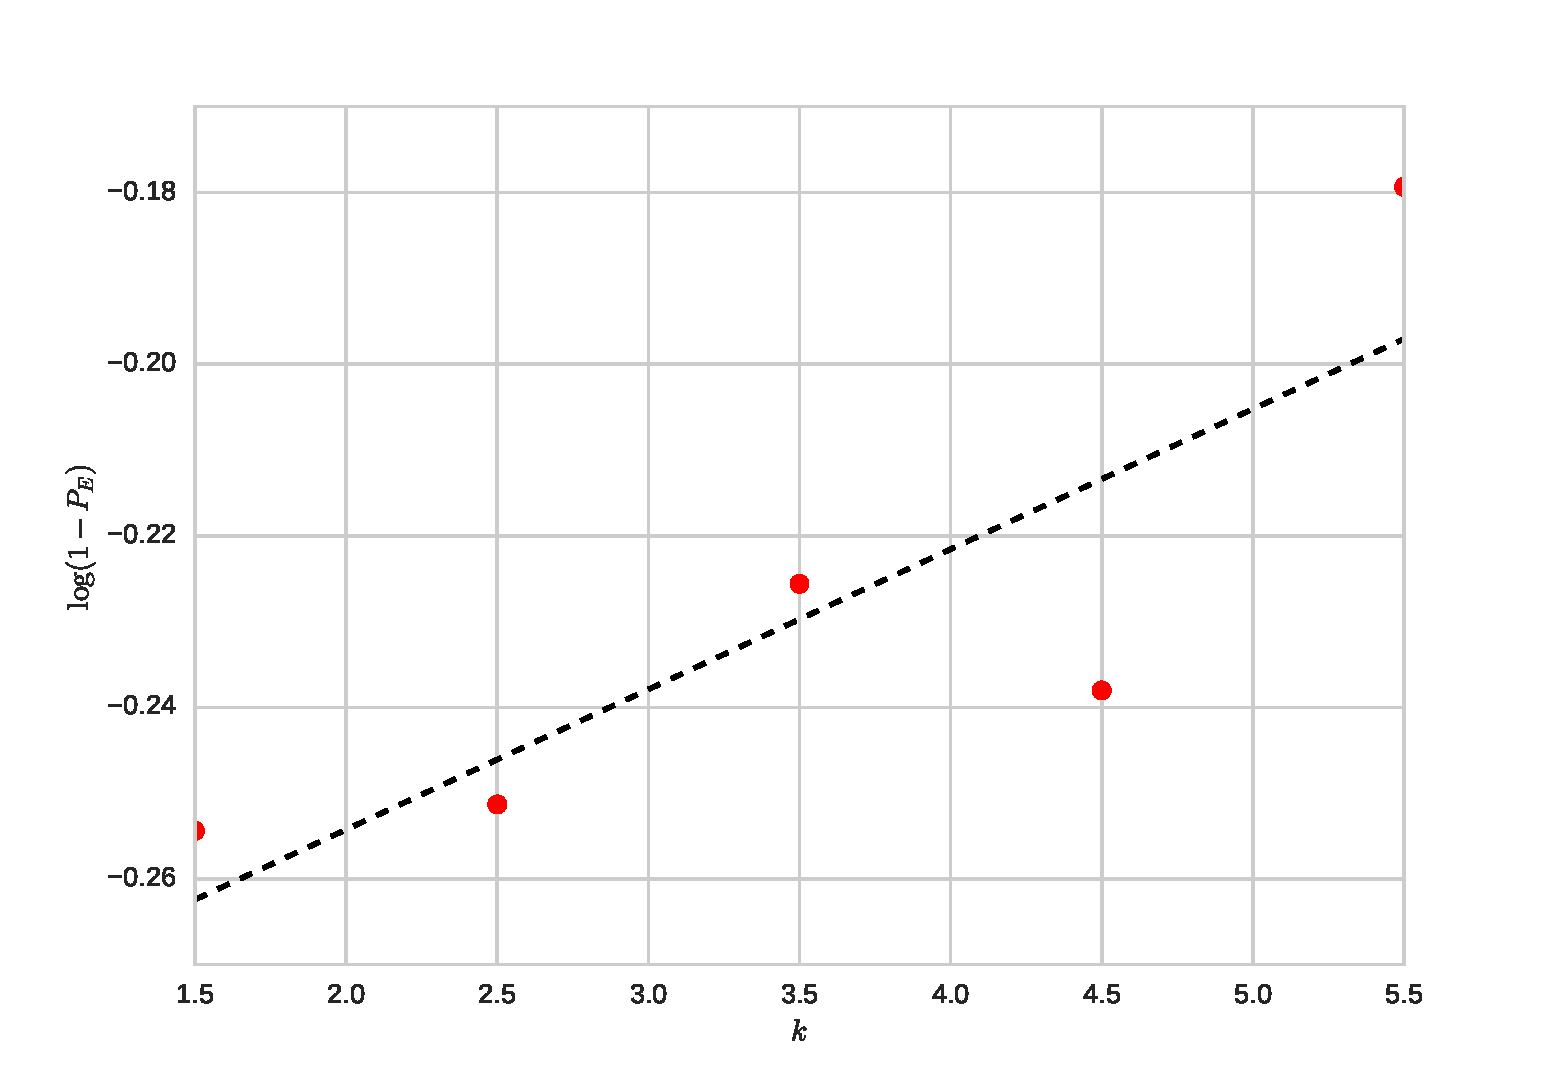
\includegraphics[width=\textwidth]{./schemes/yeast_Y2H.pdf}
        \caption{\label{fig:y2h} Y2H}
    \end{subfigure}
    \caption{\label{fig:fit} Ajustes lineales de las probabilidades de no-esencialidad y grado (ver ec. \ref{eq:ne}. 
    (a) $\alpha = 0.53 \pm 0.002 $ y $\beta = 0.26 \pm 0.017$; (b) $\alpha = 0.073 \pm 0.008$ y $\beta = 0.224 \pm 0.043$. 
    Debido al comportamiento irregular, Y2H ha sido excluida del an\'alisis.}
\end{figure}


%--- simulaciones de redes random

\subsection{M\'etodo de simulaciones}
\label{sec:simulacion}

Es dif\'icil identificar interacciones esenciales (PPIs) experimentalmente en la escala gen\'omica, dado que esta identificaci\'on requiere la demostraci\'on de que romper el enlace entre prote\'inas esenciales sin afectar otros aspectos de las funciones prote\'icas causa letalidad o infertilidad.

Aqu\'i usamos un m\'etodo computacional para evaluar la prevalecencia de enlaces esenciales PPIs y la contribuci\'on de PPIs esenciales a la esencialidad de genes al nivel gen\'omico.

Nuestro an\'alisis se enfoca en las redes {\it LIT} y {\it Y2H}.
%, excluyendo a la red {\it AP-MS}, como se hizo en la secci\'on anterior. 
%Tambi\'en excluimos a la red {\it LIT-Reguly} debido 

Como se mencion\'o antes, dos prote\'inas que forman un enlace esencial PPI deben ser esenciales.
Por el contrario, las interacciones entre prote\'inas esenciales (IBEPs, {\it Interaction Between Essential Proteins}, por sus siglas en ingl\'es) pueden o no ser esenciales, dado que la esencialidad de una prote\'ina puede deberse a otros factores adem\'as de las PPIs.
Esta caracter\'istica nos permite estimar el n\'umero de PPIs esenciales en una red, dado queque el n\'umero de IBEPs crece con el n\'umero de PPIs esenciales.

Dado el n\'umero total de interacciones IBEPs $N_{ie}$ para cada red, generamos una red de control haciendo un recableado de los enlaces, manteniendo la distribuci\'on de grado $P(k)$ para cada nodo.
Repitiendo este procedimiento 5000 veces (1000 para la red {\it Y2H}), obtenemos la distribuci\'on del n\'umero ($n_{ie}$) de enlaces esenciales (IBEPs) en redes recableadas al azar.
En todos los caso, el m\'aximo valores de la distribuci\'on no supera el caso de la red real; es decir, $max(n_{ie}) < N_{ie}$ siempre.
Este exceso del caso real tambi\'en se observa en otros casos de PPIs de levadura y en PPIs de nematodos {\bf CITAR 14 y 15, ver p. 2}.

Siguiendo el m\'etodo de \cite{he2006}, determinamos la fracci\'on de interacciones esenciales PPI como $\alpha = (N_{ie} - <n_{ie}>)/(N_{nod})$, siendo $N_{tot}$ el n\'umero total de nodos de la red.
Los valores para las diferentes redes se muestran en la tabla \ref{tab:probas}.


%--- overlapping
% NOTE: sacado de:
% ./beta -- ...
Notar que algunos nodos resultaron afectados por ambos factores; es decir por asignaci\'on random y por PPIs esenciales. 
En particular, para el caso {\it Y2H} es del $22 \pm 6$ \%, y para {\it LIT} es del $7.10 \pm 3.04$.

\begin{figure}
\centering
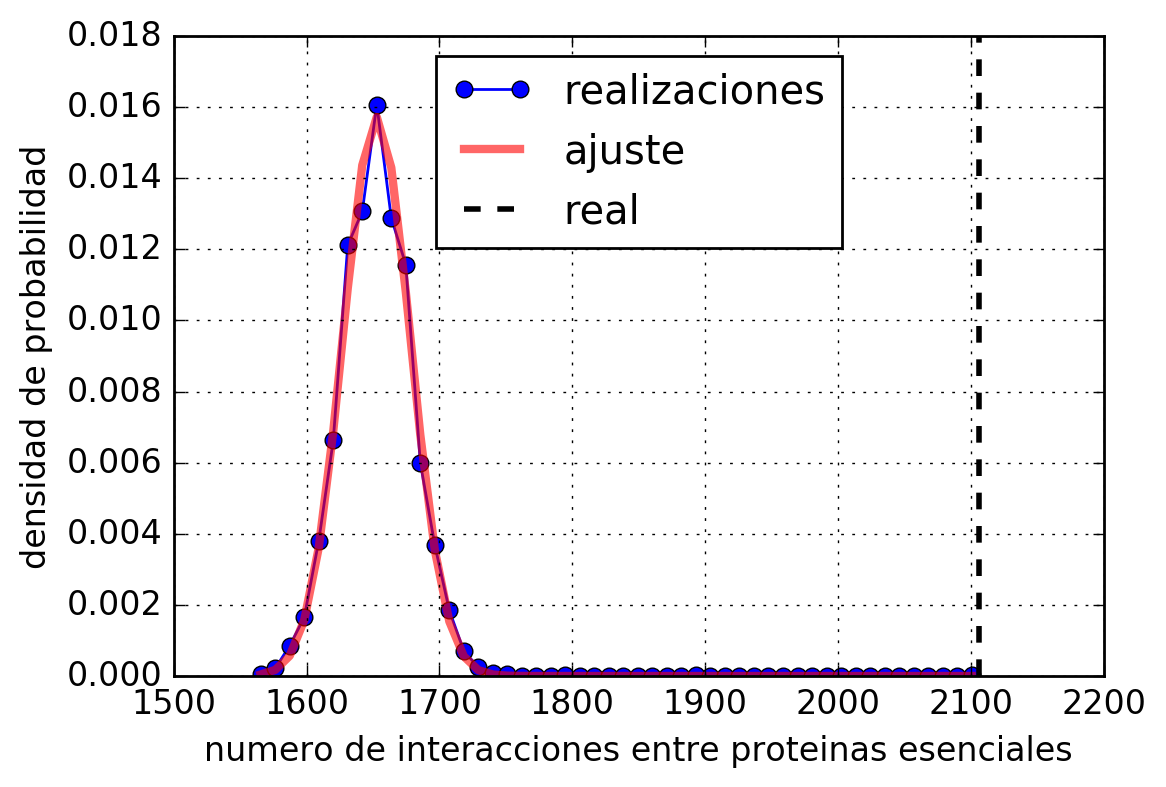
\includegraphics[scale = 0.6]{figuras/hist_LIT} 
\includegraphics[scale = 0.6]{figuras/hist_Y2H} \\
\caption{Distribuciones observadas del n\'umero de interacciones esenciales para los casos random de la redes estudiadas mediante simulaciones, para investigar las probabilidad $\alpha$ y $\beta$ de la red.}
\label{fig:remocion_alternativo}
\end{figure}

%EO



\subsection{Discuci\'on}
\begin{table}[!ht]
    \centering
    \caption{\label{tab:probas} Resumen de probabilidades estimadas para cada red a trav\'es de m\'etodo de ajuste
y simulaciones.}
    {\scriptsize
    \begin{tabularx}{.9\columnwidth}{XlccXccX}
        \hline\hline
        &               &  \multicolumn{2}{c}{Simulaci\'on}  &&  \multicolumn{2}{c}{Ajuste}          &      \\
        \cline{3-4} \cline{6-7}
        &               &   $\alpha$    & $\beta$        &&   $\alpha$       &       $\beta$     & \\
        \hline
        & LIT\_Reguly   & --  & --     && 5.3$ \pm$ 0.2  & 2.6 $\pm$ 1.7       &               \\
        & LIT           & 29 $\pm$ 1 & 7 $\pm$ 3   && 7.3 $\pm$ 0.8  & 24.4 $\pm$ 4.3       &               \\
        & Y2H           &  7 $\pm$ 1 & 14 $\pm$ 6  &&    ---             &   ---              &               \\
        \hline\hline
    \end{tabularx}
    }
\end{table}


\begin{table}[!ht]
    \centering
    \caption{\label{tab:pairs} Cantidad de pares totales o de igual caracteristica (ambos esenciales o ambos no esenciale)
    en comparaci\'on al valor estimado desprendido de la hipotesis de \citet{he2006}.}
    {\scriptsize
    \begin{tabularx}{.9\columnwidth}{XlccccX}
        \hline\hline
        &               & Pares   & Pares del   & \multicolumn{2}{c}{Pares esperados del mismo tipo }             \\ 
        \cline{5-6}
        &               & Totales & mismo tipo  & Simulaci\'on  &        Ajuste         &      \\
        \hline
 %       & AP-MS         & 11613 & 5924 & &  &            \\ 
        & LIT\_Reguly   & 10777   & 6187        &               &         5716          &               \\
        & LIT           & 1858    & 1059        &               &          963          &               \\
        & Y2H           & 2258    & 1493        &               &                       &               \\
        \hline\hline
    \end{tabularx}
    }
\end{table}



\bibliographystyle{plainnat}
\bibliography{biblio}
\end{document}
